{\bfseries Производственные и обрабатывающие отрасли}

{\bfseries \emph{Технология продовольственных продуктов}}

{\bfseries Диханбаева Ф.Т., Есиркеп Г.Е., Жунусова Г.С., Ж.Нармандах,
Калемшарив Б.}

\emph{ҚЫМЫЗ ӨНДІРІСІНДЕ ТАБИҒИ ҚОСПАЛАРДЫ
ПАЙДАЛАНУ.........................................................}

{\bfseries Турганбаева Н.К., Элеманова Р.Ш., Дюшеева Н.С.}

\emph{К ВОПРОСУ ХАРАКТЕРИСТИКИ МОЛОКА ОСЛИЦ КЫРГЫЗСКОЙ
ПОПУЛЯЦИИ\ldots\ldots\ldots\ldots\ldots\ldots.}

{\bfseries Альжаксина Н.E., Далабаев A.Б., Хастаева A.Ж.}

\emph{ГРЕК ЖАҢҒАҒЫ НЕГІЗІНДЕГІ ӨСІМДІК СУСЫНЫНЫҢ ТАҒАМДЫҚ ЖӘНЕ
БИОЛОГИЯЛЫҚ ҚҰНДЫЛЫҒЫН
АНЫҚТАУ№...................................................................................................................}

{\bfseries Отуншиева А.Е. , Болегенова С.А., Ламоткин С.А., Ветохин С.С.,
А.А. Ешанкулов}

\emph{ҚАЗАҚСТАНДЫҚ МАҚТА МАЙЫ ЖӘНЕ РЕСЕЙЛІК АРЫШ МАЙЫНЫҢ НЕГІЗІНДЕ
ТЕҢЕСТІРІЛГЕН МАЙ ҚЫШҚЫЛДЫ ҚҰРАМЫ БАР ӨСІМДІК МАЙЛАРЫ ҚОСПАЛАРЫНЫҢ ЖАҢА
ТҮРЛЕРІН
ӘЗІРЛЕУ.......................................................................................................................}

{\bfseries Tultabayeva T.Ch., Zhakupova G.N., Kokumbekova N., Sagandyk
A.T., Muldasheva A.H.,}

{\bfseries Akhmetzhanova A.T.}

\emph{STUDYING EFFECT OF FREEZE DRYING ON THE CHEMICAL COMPOSITION OF
COW
COLOSTRUM\ldots\ldots\ldots\ldots\ldots\ldots\ldots\ldots\ldots\ldots\ldots\ldots\ldots\ldots\ldots\ldots\ldots\ldots\ldots\ldots\ldots\ldots\ldots\ldots\ldots\ldots\ldots\ldots\ldots\ldots\ldots\ldots\ldots\ldots\ldots\ldots\ldots\ldots\ldots\ldots..}

{\bfseries Yessembek M.Zh., Tarabayev B.K., Omaraliyeva A.M.}

\emph{INCREASING OF MICROBIOLOGICAL STABILITY OF BREAD WITH USING
SECONDARY RAW MATERIALS FROM CEREAL PROCESSING}

{\bfseries .}

{\bfseries \emph{Технология продовольственных продуктов}}\newpage
{\bfseries ҒТАМР 65.63.03}

{\bfseries ҚЫМЫЗ ӨНДІРІСІНДЕ ТАБИҒИ ҚОСПАЛАРДЫ ПАЙДАЛАНУ}

{\bfseries \textsuperscript{1}Ф.Т. Диханбаева , \textsuperscript{2}Г.Е.
Есиркеп, \textsuperscript{2}Г.С. Жунусова,
\textsuperscript{2}Ж.Нармандах, \textsuperscript{3}Б.Калемшарив}

\textsuperscript{1}Алматы технологиялық университеті, Алматы, Қазақстан,

\textsuperscript{2}Қ. Құлажанов атындағы Қазақ технология және бизнес
университеті, Астана, Қазақстан,

\textsuperscript{3}С. Сейфуллин атындағы Қазақ агротехникалық зерттеу
университеті, Астана, Қазақстан

Корреспондент-автор: fatima6363@mail.ru

Берілген мақалада зерттеудің негізгі мақсаты -- адам денсаулығына
пайдалы әсер ететін бие сүті және қымызды өндірудің дәстүрлі әдісін
қолдана отырып қара өрік қосылған қымызды алудың сапасы мен
технологиясын жаңарту, жаңа құрамды бие сүтінен қара өрік ұнтағы
араласқан үлгілеріне арналған ғылыми негізделген рецепттерді құрастырып,
пробиотикалық ашытылған бие сүтін дайындау болып табылады.

Соңғы уақытта бие сүтін өндіруге қызығушылық арта түсті, себебі оның
құрамында көптеген құнды қоректік заттар бар, сонымен қатар, денсаулықты
жақсартатын пайдасы зор. Адам мен бие сүтіндегі Ca-P қатынасы сиыр
сүтіндегі қатынаспен салыстырғанда Ca-ны сіңіру үшін қолайлы екені
көрсетілді.

Зерттеу кезеңі нәтижесінде пробиотикалық ашытылған бие сүті, қара өрік
ұнтағы, жоғары талшықты және пробиотикалық ашытылған бие сүті
дайындалып, қара өрік қосылған қымызды дайындау технологиясы үлгілік
сызбасы әзірленді.

Осылайша, қымыз өнімінің технологиясын әзірлеу жоғарғы тұтынушылық
қасиеттері бар функционалды тамақ өнімдерін құрудың жаңа және
перспективалы тәсілі болып табылады.

{\bfseries Түйін сөздер:} сүт, бие сүті, сиыр сүті, ана сүті, қымыз, қара
өрік ұнтағы, функционалдық тамақ, пробиотикалық, пребиотикалық.

{\bfseries ИСПОЛЬЗОВАНИЕ НАТУРАЛЬНЫХ ДОБАВОК В ПРОИЗВОДСТВЕ КУМЫСА}

{\bfseries \textsuperscript{1}Ф.Т. Диханбаева, \textsuperscript{2}Г.Е.
Есиркеп, \textsuperscript{2}Г.С. Жунусова, \textsuperscript{2}Ж.
Нармандах, \textsuperscript{3}Б. Калемшарив}

\textsuperscript{1}Алматинский технологический университет, Алматы,
Казахстан,

\textsuperscript{2}Казахский университет технологии и бизнеса им.
К.Кулажанова, Астана, Казахстан,

\textsuperscript{3}Казахский исследовательский аграрный университет им.
С. Сейфуллина, Астана, Казахстан,

e-mail: fatima6363@mail.ru

Основной целью исследования в данной статье является исследование
качества и разработка технологии напитка традиционным способом из
кошерного молока и кошерной сливы, благотворно влияющей на здоровье
человека, создание научно обоснованных рецептур, получение новых
композиций на основе кобыльего молока смешанных с порошком из сливы и
приготовление пробиотического ферментированного кобыльего молока.

В последнее время возрос интерес к производству кобыльего молока,
поскольку оно содержит множество ценных питательных веществ, обладающее
оздоровительными свойствами. Было показано, что соотношение Ca-P в
человеческом и кобыльем молоке более благоприятно для усвоения
организмом Ca, чем в коровьем молоке.

В результате исследовательской работы был разработан напиток из
кобыльего молока ферментированного пробиотиками, с использованием
сливового порошка и меда, и разработана технологическая схема
приготовления кошерного молока со сливой.

Таким образом, разработка технологии производства кумыса является новым
и перспективным направлением при создании функциональных продуктов
питания с высокими потребительскими свойствами.

{\bfseries Ключевые слова:} молоко, кобылье молоко, коровье молоко, грудное
молоко, кумыс, порошок чернослива, функциональная пища, пробиотик,
пребиотик.

{\bfseries THE USE OF NATURAL ADDITIVES IN THE PRODUCTION OF KUMISS}

{\bfseries \textsuperscript{1}F.T. Dikhanbayeva, \textsuperscript{2}G.E.
Esirkep, \textsuperscript{2}G.S. Zhunusova,
\textsuperscript{2}Zh.Narmandakh, \textsuperscript{3}B. Kalemshariv}

\textsuperscript{1}Almaty Technological University, Almaty, Kazakhstan,

\textsuperscript{2}Kazakh University of Technology and Business named
after K. Kulajanov, Astana, Kazakhstan,

\textsuperscript{3}Kazakh Research Agrarian University named after S.
Seifullin, Astana, Kazakhstan,

e-mail: fatima6363@mail.ru

The main goal of the research in this article is to update the quality
and technology of producing kosher with plums using the traditional
method of producing mare\textquotesingle s milk and kosher, which has a
beneficial effect on human health, to create scientifically based
recipes for samples of new composition of mare\textquotesingle s milk
mixed with plum powder, and to prepare probiotic fermented
mare\textquotesingle s milk. is.

Recently, there has been an increased interest in the production of
mare\textquotesingle s milk, because it contains many valuable
nutrients, as well as health-improving properties. The Ca-P ratio in
human and mare\textquotesingle s milk has been shown to be more
favorable for Ca absorption than that in cow\textquotesingle s milk.

As a result of the research period, probiotic-fermented
mare\textquotesingle s milk, plum powder, high-fiber and
probiotic-fermented mare\textquotesingle s milk were prepared, and a
sample drawing of the technology of preparation of kosher with plum was
developed.

Thus, the development of kumif product technology is a new and promising
way to create functional food products with high consumer properties.

{\bfseries Keywords:} milk, mare\textquotesingle s milk,
cow\textquotesingle s milk, breast milk, koumiss, prune powder,
functional food, probiotic, prebiotic.

{\bfseries Кіріспе.} Сүт -- аналық сүтқоректілердің ұрпақтарының қоректенуі
үшін бөлетін сұйықтық. Сүтқоректілердің сүтінің құрамдас бөліктерінің
көпшілігі су, май, ақуыз, көмірсулар, минералды және дәруменді заттар
болып табылады. Бие сүті («саумал») -- физиологиялық, нәзік және жай
ассимиляцияланған биологиялық белсенді өнім {[}1{]}.

Бие сүті құрамында фосфолипидтер мен А дәруменінің жоғары болуына
байланысты қышқылға қарсы қасиетке ие. Бие сүтін өкпе ауруы бар, әсіресе
туберкулезбен ауыратын науқастарды емдеу үшін пайдалану Ресей мен
Моңғолия аумағында ұзақ уақыт бойы қолданылып келеді. Сонымен қатар,
кейбір зерттеулерде бие сүтін пайдалану арқылы анемия, нефрит, диарея,
гастрит және басқа ас қорыту ауруларымен күресу мүмкіндігі бар екендігін
хабарлады {[}1{]}.

Бие сүтінің құрамы адам сүтіне ұқсас және ол лактоферрин, лизоцим, ω-3
және ω-6 май қышқылдарының жоғары концентрациясының болуына байланысты
көптеген биологиялық функцияларды орындауға қабілетті болуы керек
{[}2{]}.

Бие сүтінің құрамында адам ағзасына қажетті 40-қа жуық биологиялық
компоненттер: аминқышқылдары, майлар, ферменттер (лизоцим, амилаза),
микроэлементтер (кальций, натрий, калий, фосфор, темір, магний, мыс,
йод, күкірт, кобальт, мырыш, бром) және дәрумендер (A, C, B1, B2, B6,
B12, E, каротиноид, фолий қышқылы) оңтайлы теңдестірілген пропорцияда
кездеседі. Бие сүті лактозаның -- 72,80 г/л, майдың -- 6,40 г/л және
ақуыздар 15,52 г/л, атап айтқанда казеиндердің -- 13,4 г/л жеткілікті
мөлшерімен сипатталады. Бие сүтінің емдік маңызы бүкіл Ресей мен Батыс
Азия аумағында аңызға айналған. Моңғол дәрігерлері бие сүтін созылмалы
жұқпалы ауруларды, бауыр және ойық жара ауруларын емдеу үшін пайдалануды
тәжірибеге айналдырған {[}3{]}.

Бие сүтінің құрамы ана сүтіне ұқсас және ол лактоферрин, лизоцим, ω-3
және ω-6 май қышқылдарының жоғары концентрациясының болуына байланысты
көптеген биологиялық функцияларды орындауға қабілетті {[}3{]}.

Бие сүтінің химиялық құрамы. Сүттің жалпы құрамы түрлер арасында
айтарлықтай өзгеретіні мойындалады, өйткені түтік бездерінің секрециясы
әрбір нақты түрдегі жаңа туған нәрестенің биологиялық процесінің
қажеттіліктерімен физиологиялық және құрылымдық түрде байланысты
{[}4{]}.

1.2-кесте бие, ана және сиыр сүтінің жалпы құрамын, 3 түрдің арасында
маңызды өзгерістер болған жерде салыстыруды көрсетеді. Бие сүтіндегі
лактозаның мөлшерін ана сүтімен салыстыруға болады, сонымен қатар, ол
сиыр сүтінен жоғары. Алайда, бие мен ана сүтінде сиыр сүтімен
салыстырғанда ақуыздар мен минералдардың деңгейі айтарлықтай төмен
(1-кестеде көрсетілген).

{\bfseries 1-кесте -- Бие, ана, сиыр сүттерінің химиялық құрамы мен
энергетикалық құндылықтары}

\begin{longtable}[]{@{}
  >{\raggedright\arraybackslash}p{(\columnwidth - 6\tabcolsep) * \real{0.2501}}
  >{\raggedright\arraybackslash}p{(\columnwidth - 6\tabcolsep) * \real{0.2500}}
  >{\raggedright\arraybackslash}p{(\columnwidth - 6\tabcolsep) * \real{0.2500}}
  >{\raggedright\arraybackslash}p{(\columnwidth - 6\tabcolsep) * \real{0.2500}}@{}}
\toprule\noalign{}
\begin{minipage}[b]{\linewidth}\raggedright
Құрамдас бөліктер
\end{minipage} & \begin{minipage}[b]{\linewidth}\raggedright
Бие сүті
\end{minipage} & \begin{minipage}[b]{\linewidth}\raggedright
Ана сүті
\end{minipage} & \begin{minipage}[b]{\linewidth}\raggedright
Сиыр сүті
\end{minipage} \\
\midrule\noalign{}
\endhead
\bottomrule\noalign{}
\endlastfoot
Май, \% & 0,5-2,0 & 3,5-4,0 & 3,5-3,9 \\
Ақуыз, \% & 1,5-2,8 & 0,9-1,7 & 3,1-3,8 \\
Лактоза, \% & 5,8-7,0 & 6,3-7,0 & 4,4-4,9 \\
Күл, \% & 0,3-0,5 & 0,2-0,3 & 0,7-0,8 \\
Энергетикалық құндылығы, ккал/кДж & 390-550 & 650-700 & 650-712 \\
\end{longtable}

Биенің уыз сүтіндегі казеин мен сарысу ақуызының арақатынасы төлдегеннен
кейін бірден 0,2:1 құрайды және ол бір апта ішінде 1,1:1-ге өзгереді.
Бие сүті салыстырмалы түрде лактозаға бай және оның көлемі лактация
уақытында ақырындап азаяды. Бие сүтінің майлылығы лактацияның
жоғарылауымен төмендейді, ал ірі қара сүті лактацияның 3 айынан кейін
белгілі минимумды көрсетеді және одан кейін жоғарылайды. Бие сүтінің
энергетикалық құрамы ана мен сиыр сүтіне қарағанда айтарлықтай төмен
болып келеді. Бие сүтінің басқа сүтқоректілермен салыстырғанда майы аз,
оның мәні небәрі 5 г/кг-дан төмен. Бие сүті күлі 0,3-0,5\% аралығында
және бұл көрсеткіш ішінара кальций мен фосфордың, ақуыздың төмен
мазмұнымен байланысты {[}5{]}.

\emph{Липидтер.} Бие сүтінің майы ана мен сиыр сүтімен салыстырғанда өте
төмен. Төлдегеннен кейін бірден уыз сүтіндегі майдың мөлшері орташа
есеппен 2,9\%, ал өтпелі сүт және қалыпты сүттің орташа мөлшері
сәйкесінше 2,1\% және 1,2\% құрады. Уыз сүті мен қалыпты бие сүті
арасында майдың құрамында айқын айырмашылықтар болған жоқ. Сүт липидтері
эмульсияланған түйіршіктер түрінде таралады және бие сүтінің май
түйіршіктерінің мөлшері шамамен 2-3 мкм құрайды. Уыз сүтіндегі сүт
майының глобулды қабығы бие сүті сияқты гликопротеинді жіптермен
қапталған, олардың ұсынылатын рөлі майдың қорытылуын күшейту үшін
липазаларды байланыстырады {[}5{]}.

\emph{Ақуыз.} Бие сүтінде сиыр сүтімен салыстырғанда жалпы ақуыз аз,
бірақ 1.3-кестеде көрсетілгендей адам сүтінен жоғары. Бие сүтінде
казеинді емес азот сарысу ақуызына да, ақуызды емес азот фракцияларына
қатысты да жоғары. Сиыр сүтінің құрамында бие мен адам сүтімен
салыстырғанда жоғары казеин бар. Бие сүтінің ақуыздары 40-60\%
казеиндерден тұрады, ол адам сүтімен сәйкес келеді (40\% казеиндер). Бие
сүтінің бос аминоалкан қышқылының фракциясы әсіресе серин мен глютамин
қышқылына бай {[}5{]}.

\emph{Май қышқылдары.} Бие сүтінің майлары қанықпаған май қышқылдарының
жоғары пайызымен сипатталады (жалпы май қышқылдары шамамен 53\%), ол ана
сүтіне ұқсас (59,5\%), бірақ сиыр сүтінен 37\% жоғары. Бие сүтіндегі
жалпы қанықпаған және қаныққан май қышқылдарының арақатынасы 1,03 пен
1,33 аралығында, ал сиыр сүтінде орташа есеппен 0,5 {[}6{]}.

Сарысу ақуызының үлесі бие сүтінде шамамен 40\% құрайды, бұл адам
сүтінен (50\%) біршама төмен және сиыр сүтінен аз. Бие сүтінің ақуыздары
сиыр, ешкі, түйе және адам сүтінің ақуыздарына қарағанда адамның
асқазан-ішек жолдарының ферменттерімен оңай қорытылады {[}6{]}.

{\bfseries 2-кесте - Бие, ана және сиыр сүттерінің ақуыздық фракциялары}

\begin{longtable}[]{@{}
  >{\raggedright\arraybackslash}p{(\columnwidth - 6\tabcolsep) * \real{0.3485}}
  >{\raggedright\arraybackslash}p{(\columnwidth - 6\tabcolsep) * \real{0.1971}}
  >{\raggedright\arraybackslash}p{(\columnwidth - 6\tabcolsep) * \real{0.2043}}
  >{\raggedright\arraybackslash}p{(\columnwidth - 6\tabcolsep) * \real{0.2501}}@{}}
\toprule\noalign{}
\begin{minipage}[b]{\linewidth}\raggedright
Құрамдас бөліктер
\end{minipage} & \begin{minipage}[b]{\linewidth}\raggedright
Бие сүті
\end{minipage} & \begin{minipage}[b]{\linewidth}\raggedright
Ана сүті
\end{minipage} & \begin{minipage}[b]{\linewidth}\raggedright
Сиыр сүті
\end{minipage} \\
\midrule\noalign{}
\endhead
\bottomrule\noalign{}
\endlastfoot
Ақуыз, г/кг & 21,4 & 14,2 & 32,5 \\
Сарысу ақуызы, г/кг & 7,8 & 7,6 & 5,7 \\
Казеин, г/кг & 10,2 & 3,7 & 25,1 \\
Ақуыз емес азот, г/кг & 2,4 & 2,9 & 1,7 \\
\end{longtable}

\emph{Дәрумендер.} Бие сүтінің дәрумендері 8-45 күндік лактация
кезіндегі қалыпты бие сүтімен салыстырғанда А, D3, C және K3
витаминдерінен 2,6, 1,7, 1,4 және 1,5 есе сәйкесінше жоғары. С
дәруменінің мөлшері де қалыпты сүтке қарағанда уыз сүтінде жоғары
болады, ал бие сүтінде сиыр сүтіне қарағанда С дәрумені жоғары болады.
Дәрумендермен байытылған бие сүтінің ұнтағы α, γ және δ токоферолдардың
ерекше жоғары деңгейіне ие. Бұл зерттеуде олар өнімнің жарамдылық
мерзімін, сондай-ақ, дайын өнімнің тағамдық сапасын арттыру үшін
қосылды. Сонымен қатар, ұнтақталған бие сүті үлгілерінің термиялық өңдеу
кезінде транс ретинолдың изомерленуіне байланысты шикі бие сүтіне
қарағанда цис/транс ретинол арақатынасы жоғары болды {[}6{]}.

Бие сүтінде сиыр сүтімен салыстырғанда А дәруменінің деңгейі ұқсас,
бірақ оның ана сүтіне қарағанда аз екенін көрсетті. Биелер жеміне
β-каротин қосу арқылы уыз сүті мен сүттегі осы дәруменнің деңгейін
жоғарылатқаны анықталды. Соңғы зерттеулердің нәтижелері D дәрумені ана
сүтімен салыстырғанда бие сүтінде көбірек болатынын көрсетті {[}7{]}.

Басқа зерттеу мәліметтері бойынша, D дәрумені қоспаларын қабылдау ерте
қатерлі ісік ауруынан болатын өлім қаупін едәуір төмендетіп, жалпы
денсаулықты жақсартатындығын анықтаған. Бие сүтінде В дәруменінің орташа
концентрациясы сипатталады, ал ана сүтінде бие сүтімен салыстырғанда бұл
дәрумен аз, ал сиыр сүтінде көп болады (кесте 3). Бие сүтіндегі
кобаламин деңгейі жоғары, ал В\textsubscript{2} және В\textsubscript{9}
дәрумендері адам мен сиыр сүтімен салыстырғанда төмен екендігі
көрсетілген {[}8{]}.

{\bfseries 3-кесте - Бие, адам және сиыр сүтіндегі суда еритін
дәрумендердің құрамын салыстыру {[}9{]}}

\begin{longtable}[]{@{}
  >{\raggedright\arraybackslash}p{(\columnwidth - 6\tabcolsep) * \real{0.3029}}
  >{\raggedright\arraybackslash}p{(\columnwidth - 6\tabcolsep) * \real{0.2427}}
  >{\raggedright\arraybackslash}p{(\columnwidth - 6\tabcolsep) * \real{0.2427}}
  >{\raggedright\arraybackslash}p{(\columnwidth - 6\tabcolsep) * \real{0.2117}}@{}}
\toprule\noalign{}
\begin{minipage}[b]{\linewidth}\raggedright
Дәрумен атауы (мкг/л)
\end{minipage} & \begin{minipage}[b]{\linewidth}\raggedright
Бие сүті
\end{minipage} & \begin{minipage}[b]{\linewidth}\raggedright
Ана сүті
\end{minipage} & \begin{minipage}[b]{\linewidth}\raggedright
Сиыр сүті
\end{minipage} \\
\midrule\noalign{}
\endhead
\bottomrule\noalign{}
\endlastfoot
Тиамин - В1 & 20-40 & 14-17 & 28-90 \\
Рибофлавин -- В2 & 10-37 & 20-60 & 116-202 \\
Ниацин -- В3 & 70-140 & 147-178 & 50-120 \\
Пантотен қышқылы -- В5 & 277-300 & 184-270 & 260-490 \\
Пиридоксин -- В6 & 30 & 11-14 & 30-70 \\
Фолий қышқылы -- В9 & 0,13 & 5,2-16 & 1-18 \\
Кобаламин -- В12 & 0,3 & 0,03-0,05 & 0,11 \\
Аскорбин қышқылы - С & 1280-8100 & 3500-10000 & 300-2300 \\
\end{longtable}

\emph{Макро және микроэлементтер.} Ана мен бие сүтіндегі минералды
заттар сиыр сүтімен салыстырғанда төмен. Катиондар түріндегі натрий қан
мен жасушадан тыс сұйықтықтың құрамдас бөлігі ретінде маңызды рөл
атқарады, катион түріндегі калий жасушаішілік сұйықтықтың тұтастығын
сақтауға қатысады. Сүт, әдетте, сүйектің өсуі мен дамуы үшін қажет
кальций мен фосфордың, сондай-ақ, сүйектің минералдануы үшін қажет
магнийдің жақсы көзі болып табылады. Минералды заттар лактацияның
бірінші аптасында ең жоғары болады, содан кейін азаяды. Бие сүтіндегі
минералдардың үлесі үнемі өзгеріп отыратындықтан, олардың орташа
концентрациясын дәл анықтау қиын.

Айта кету керек, бірлік үлгісі бүкіл лактацияның өкілі емес, керісінше
лактацияның белгілі бір кезеңі үшін. Сонымен қатар, лактацияның бірінші
аптасында Ca:P қатынасының 1,45:1-ден 15-17 аптада 1,3:1-ге дейін
өзгеруін байқады, бұл адамдарда осы элементтердің оңтайлы қатынасына
жақын (1:1-ден 1,3:1-ге дейін). Сонымен қатар, Ca:Mg қатынасы 11:1-ден
16:1-ге дейін өзгерді. Бие тұқымына байланысты минералды құрамдағы
айырмашылықтар 1.5-кестеде көрсетілген. Кальцийдің ең жоғары мөлшері
бардигиано биелері мен итальяндық Қайың тұқымдарының сүтінде байқалады.
Магний мен мырыштың ең төменгі мәндері Араб биелерінде байқалды
(4-кесте) {[}10{]}.

{\bfseries 4-кесте - Әр түрлі тұқымды бие сүтіндегі макро және
микроэлементтердің орташа мөлшері {[}10{]}}

\begin{longtable}[]{@{}
  >{\raggedright\arraybackslash}p{(\columnwidth - 18\tabcolsep) * \real{0.2226}}
  >{\raggedright\arraybackslash}p{(\columnwidth - 18\tabcolsep) * \real{0.1436}}
  >{\raggedright\arraybackslash}p{(\columnwidth - 18\tabcolsep) * \real{0.0880}}
  >{\raggedright\arraybackslash}p{(\columnwidth - 18\tabcolsep) * \real{0.0889}}
  >{\raggedright\arraybackslash}p{(\columnwidth - 18\tabcolsep) * \real{0.0887}}
  >{\raggedright\arraybackslash}p{(\columnwidth - 18\tabcolsep) * \real{0.0751}}
  >{\raggedright\arraybackslash}p{(\columnwidth - 18\tabcolsep) * \real{0.0872}}
  >{\raggedright\arraybackslash}p{(\columnwidth - 18\tabcolsep) * \real{0.0755}}
  >{\raggedright\arraybackslash}p{(\columnwidth - 18\tabcolsep) * \real{0.0650}}
  >{\raggedright\arraybackslash}p{(\columnwidth - 18\tabcolsep) * \real{0.0654}}@{}}
\toprule\noalign{}
\multirow{2}{*}{\begin{minipage}[b]{\linewidth}\raggedright
Жылқы тұқымы
\end{minipage}} &
\multirow{2}{*}{\begin{minipage}[b]{\linewidth}\raggedright
Лактация уақыты
\end{minipage}} & \multicolumn{8}{l@{}}{%
\begin{minipage}[b]{\linewidth}\raggedright
Макро және микроэлементтер (мг/дл)
\end{minipage}} \\
& & \begin{minipage}[b]{\linewidth}\raggedright
Сa
\end{minipage} & \begin{minipage}[b]{\linewidth}\raggedright
P
\end{minipage} & \begin{minipage}[b]{\linewidth}\raggedright
Mg
\end{minipage} & \begin{minipage}[b]{\linewidth}\raggedright
Na
\end{minipage} & \begin{minipage}[b]{\linewidth}\raggedright
K
\end{minipage} & \begin{minipage}[b]{\linewidth}\raggedright
Zn
\end{minipage} & \begin{minipage}[b]{\linewidth}\raggedright
Fe
\end{minipage} & \begin{minipage}[b]{\linewidth}\raggedright
Cu
\end{minipage} \\
\midrule\noalign{}
\endhead
\bottomrule\noalign{}
\endlastfoot
Араб & 2-30 & 914 & 394 & 59 & 132 & 632 & 0,89 & 1,46 & 0,25 \\
Жартылық & 3-180 & 787 & 504 & 75 & 171 & 701 & - & - & - \\
Прежевальский & 85-250 & 804 & 419 & 62 & 137 & 344 & 1,9 & 1,10 &
0,23 \\
Асыл тұқымды & 6-120 & 811 & 566 & 53 & 140 & 410 & 1,9 & 0,27 & 0,25 \\
Шетланд пони & 6-120 & 857 & 418 & 77 & 127 & 250 & 1,7 & - & 0,37 \\
Бардигиано & 5-35 & 1220 & 668 & - & 198 & 662 & 2,79 & 1,06 & 1,06 \\
Итальяндық қайың жылқысы & 5-35 & 1155 & 678 & - & 167 & 573 & 2,95 &
1,47 & 0,73 \\
Хафлингер & 4-180 & 802 & 593 & 77 & 181 & 443 & - & - & - \\
\end{longtable}

{\bfseries 5-кесте - Бие, ана және сиыр сүттеріндегі минералды
заттар{[}10{]}}

\begin{longtable}[]{@{}
  >{\raggedright\arraybackslash}p{(\columnwidth - 6\tabcolsep) * \real{0.3333}}
  >{\raggedright\arraybackslash}p{(\columnwidth - 6\tabcolsep) * \real{0.2427}}
  >{\raggedright\arraybackslash}p{(\columnwidth - 6\tabcolsep) * \real{0.1972}}
  >{\raggedright\arraybackslash}p{(\columnwidth - 6\tabcolsep) * \real{0.2268}}@{}}
\toprule\noalign{}
\begin{minipage}[b]{\linewidth}\raggedright
Минерал атауы (мг/100 мл)
\end{minipage} & \begin{minipage}[b]{\linewidth}\raggedright
Бие сүті
\end{minipage} & \begin{minipage}[b]{\linewidth}\raggedright
Ана сүті
\end{minipage} & \begin{minipage}[b]{\linewidth}\raggedright
Сиыр сүті
\end{minipage} \\
\midrule\noalign{}
\endhead
\bottomrule\noalign{}
\endlastfoot
Кальций (Ca & 50-135 & 28-34 & 112-123 \\
Фосфор (P) & 20-121 & 14-43 & 59-119 \\
Калий (K) & 25-87 & 53-62 & 106-163 \\
Магний (Mg) & 3-12 & 3-4 & 7-12 \\
Натрий (Na) & 8-85 & 10-18 & 58 \\
Хлор (Cl) & 19 & 60-63 & 100-119 \\
Темір (Fe) & 0.02-0.15 & 0.04-0.2 & 0.03-0.1 \\
Мырыш (Zn) & 0.09-0.64 & 0.2-0.4 & 0.3-0.55 \\
Мыс (Cu) & 0.02-0.11 & 0.02-0.06 & 0.01-0.08 \\
\end{longtable}

Бие, сиыр және ана сүттеріндегі минералды құрамда айтарлықтай
айырмашылықтар бар: бие сүтіндегі минералдардың көпшілігінің
концентрациясы адамға қарағанда жоғары, бірақ сиыр сүтіне қарағанда
айтарлықтай төмен (5-кесте). Кейбір зерттеулер сиыр сүтінде шамамен 50\%
Ca және бие сүтінен екі есе көп P және K бар екенін көрсетті, бірақ бие
сүтінде ана сүтінен шамамен 2 есе көп Ca және P бар. Ана мен бие
сүтіндегі Ca-P қатынасы сиыр сүтіндегі қатынаспен салыстырғанда Ca-ны
сіңіру үшін қолайлы екені хабарланды. Барлық қарастырылған сүт
түрлеріндегі микроэлементтердің концентрациясы төмен. Сүт минералдарының
биожетімділігіне сүттің басқа компоненттерінің құрамы сияқты әртүрлі
факторлар әсер етуі мүмкін {[}11{]}.

Басқа зерттеу мәліметтері бойынша, D дәрумені қоспаларын қабылдау
қатерлі ісік ауруынан болатын өлім қаупін едәуір төмендетіп, жалпы
денсаулықты жақсартатындығын анықтаған. Бие сүтінде В дәруменінің орташа
концентрациясы сипатталады, ал адам сүтінде бие сүтімен салыстырғанда
бұл дәрумен аз, ал сиыр сүтінде көп болады {[}12{]}.

Бие сүтінің құрамы адам сүтіне ұқсас және ол лактоферрин, лизоцим, ω-3
және ω-6 май қышқылдарының жоғары концентрациясының болуына байланысты
көптеген биологиялық функцияларды орындауға қабілетті {[}13{]}.

Ара балы -- көмірсулардың, минералдардың, ферменттердің және
дәрумендердің оңтайлы арақатынасы бар ара шаруашылығының ең құнды
өнімдерінің бірі. Халықтың 70\%-дан астамы балды үнемі жейді, бұл
бірінші кезекте қажет емес өнім үшін жоғары көрсеткіш тұтынушылардың
айқын емдік-профилактикалық және диеталық қасиеттерін күтуіне
байланысты. Жоғары бағамен бірге бұл оны бұрмалауға тартымды етеді.
Мысалы, балдағы ара азығына тағамдық қантты жасанды түрде қосқанда,
олигосахаридтердің мөлшері артады, мұндай балды тұтыну қант диабетімен
ауыратын адамдар үшін қауіпті болуы мүмкін {[}13{]}.

Жұмыстың мақсаты: қымыз және омарта шаруашылығы өнімдері негізінде жаңа
бие сүтнен жасалған өнімдерінің ассортиментін кеңейту

{\bfseries Материалдар мен әдістер.}

Зерттеу нысаны:

\begin{itemize}
\item
  Алматы облысының шаруа қожалықтарынан алынған бие сүті;
\item
  Қарақұмық балы;
\item
  Жаңа қарақұмық балы қосылып әзірленген қымыз.
\end{itemize}

Зерттеу объектілерінің сынамаларын алу және оларды талдауға дайындау ҚР
СТ ISO 707-2011 Сүт және сүт өнімдері стандартына сәйкес жүргізілді.

Бие сүті мен жаңа қымыз үлгілерінің органолептикалық көрсеткіштер ҚР СТ
1732-2007 негізінде, ақуыздың массалық үлесі МЕМСТ 34454-2018 бойынша
Кьельдал әдісімен, майдың массалық үлесі - МЕМСТ 5867-90 сәйкес
қышқылдық әдіспен, лактозаның массалық үлесі МЕМСТ Р 54760-2011
өнімділігі жоғары сұйық хроматография әдісімен анықталды.

Титрлеу қышқылдығы МЕМСТ 3624-92 бойынша анықталды. Әдіс фенолфталеин
индикаторының қатысуымен өнімнің құрамындағы қышқылдар мен олардың
тұздарын күйдіргіш сілтінің ерітіндісімен бейтараптандыруға негізделген.

Зерттеу жұмысына талдаулар жалпы зерттеудің стандартты және жалпы
қабылданған әдістерін қолдана отырып, Алматы технологиялық
университетінің «Тамақ қауіпсіздігі» ғылыми зерттеу институтының
аккредиттелген зертханасында жүргізілді.

Зерттеу нәтижелері 3-5 рет қайталана отырып орындалып, орташа
арифметикалық мәндері алынды.

{\bfseries Талқылау мен нәтижелер.} Зерттеуге алынған табиғи қоспа
қарақұмық балымен байытылған қымыздың негізгі шикізаты болып табылатын
бие сүтінің физико-химиялық көрсеткіштері келесідей болды: май мөлшері -
1,0 - 1,5\%, ақуыз - 1,8 - 2,0\%, лактоза - 6,7-6,8\%; титрлеу
қышқылдылығы - 6°Т, сүттің тығыздығы - 1029 кг/м\textsuperscript{3}
аралығында болды. Алынған нәтижелер қымыз өндіруге арналған бие сүтінің
ҚР СТ 1005-98 «Бие сүті» нормативтік құжатындағы талаптарға сай келеді.

Зерттеуіміздің келесі кезегінде қымызға қосылатын қарақұмық балының
оңтайлы дозасын анықтау мақсатында өнімнің органолептикалық
сипаттамаларын бағалау бойынша бірқатар тәжірибелер жүргізілді. 5\%,
6\%, 8\% мөлшерінде келесі үлгілер зерттелді. Өнімнің органолептикалық
сипаттамалары 6-кестеде көрсетілген.

{\bfseries 6-кесте - Қымызға қосылған қарақұмық балының органолептикалық
көрсеткіштерге әсері}

\begin{longtable}[]{@{}
  >{\raggedright\arraybackslash}p{(\columnwidth - 10\tabcolsep) * \real{0.0577}}
  >{\raggedright\arraybackslash}p{(\columnwidth - 10\tabcolsep) * \real{0.1400}}
  >{\raggedright\arraybackslash}p{(\columnwidth - 10\tabcolsep) * \real{0.3496}}
  >{\raggedright\arraybackslash}p{(\columnwidth - 10\tabcolsep) * \real{0.1976}}
  >{\raggedright\arraybackslash}p{(\columnwidth - 10\tabcolsep) * \real{0.1368}}
  >{\raggedright\arraybackslash}p{(\columnwidth - 10\tabcolsep) * \real{0.1184}}@{}}
\toprule\noalign{}
\endhead
\bottomrule\noalign{}
\endlastfoot
№ & Бал мөлшері, \% & Сыртқы түрі және консистенциясы & Дәмі және иісі &
Түсі & Балл \\
1 & 5 & Сұйық, біртекті, газдалған, аздап көбіктенетін, ақуыз үлпектері
мен май түйіршіктері жоқ & Сүтқышқылды, қышқыл & Ақ түсті сәл көкшіл &
4 \\
2 & 6 & Сұйық, біртекті, газдалған, аздап көбіктенетін, ақуыз үлпектері
мен май түйіршіктері жоқ & Сүтқышқылды, қышқыл & Ақ түсті сарғыш кремді
реңкті & 5 \\
3 & 8 & Сұйық, біртекті, газдалған, аздап көбіктенетін, ақуыз үлпектері
мен май түйіршіктері жоқ & Сүтқышқылды, қышқыл & Ақ түсті сәл ақшыл
қоңыр реңкті & 4 \\
\end{longtable}

Қарақұмық балдың массалық үлесі 6\% болатын үлгілер дәм тату кезінде ең
жоғары балл жинады. Ең аз ұпай санында 5\%, 8\% мөлшерінде қоспасы бар
үлгілер болды, өйткені олар балдың әлсіз және айқын дәмі бар. Іріктеу
нәтижелері бойынша қымыз сусыны үшін дозаның ең жақсы нұсқасы болып 6\%
таңдалды. Дәл осы арақатынаста өнім жағымды дәмге ие болды.

Алынған нәтижелер негізінде жаңа табиғи қоспамен байытылған қымыздың
рецептурасы мен технологиялық сұлбасы әзірленді.

Өнімнің рецепті белсенді негізгі ингредиентті (немесе ингредиенттердің
комбинациясын), формасы мен беріктігін білдіреді. Сапаны бақылау
бастапқы материалдың, аралық өнімдердің, орауыш материалдың және дайын
өнімнің сәйкестігі, беріктігі, тазалығы және басқа да сипаттамалары
бойынша белгіленген ерекшеліктерге сәйкестігін қамтамасыз ету үшін
спецификацияны анықтау, сынамаларды алу, тестілеу және аналитикалық
тазалауды қоса алғанда, қабылданатын барлық шараларды білдіреді.

Бұл зерттеу жұмысында біз бие сүті және қымызды өндірудің дәстүрлі
әдісін қолдана отырып қарақұмық балы қосылған қымызды алудың сапасы мен
технологиясын жаңарту мақсатында, жаңа құрамды рецептін «ҚР СТ 1081-2002
тамақ өнімдеріне арналған технологиялық нұсқаулықтар мен рецептураларды
әзірлеу тәртібі. Негізгі ережелер» Нормативті-техникалық құжатқа сүйене
отырып құрастырдық (7-кесте).

Зерттеуге алынған бие сүті мен қымыз үлгілерінен бөлек, барлығы 3-4
эксперименттік рецепт үлгілері құрастырылып, олардың ішінен үшінші үлгі
сенсорлық бағалауға сәйкес ең тартымды деген нәтижемен келесі реттік
зерттеу жұмыстарын жүргізуге таңдап алынды.

{\bfseries 7-кесте - Қарақұмық балы қосылған қымызды әзірлеуге ұсынылатын
рецептура үлгілері}

\begin{longtable}[]{@{}
  >{\raggedright\arraybackslash}p{(\columnwidth - 8\tabcolsep) * \real{0.2693}}
  >{\raggedright\arraybackslash}p{(\columnwidth - 8\tabcolsep) * \real{0.1807}}
  >{\raggedright\arraybackslash}p{(\columnwidth - 8\tabcolsep) * \real{0.1942}}
  >{\raggedright\arraybackslash}p{(\columnwidth - 8\tabcolsep) * \real{0.1941}}
  >{\raggedright\arraybackslash}p{(\columnwidth - 8\tabcolsep) * \real{0.1616}}@{}}
\toprule\noalign{}
\begin{minipage}[b]{\linewidth}\raggedright
Шикізат
\end{minipage} & \begin{minipage}[b]{\linewidth}\raggedright
№1 үлгі /бақылау/
\end{minipage} & \begin{minipage}[b]{\linewidth}\raggedright
№ 2 үлгі
\end{minipage} & \begin{minipage}[b]{\linewidth}\raggedright
№ 3 үлгі
\end{minipage} & \begin{minipage}[b]{\linewidth}\raggedright
№ 4 үлгі
\end{minipage} \\
\midrule\noalign{}
\endhead
\bottomrule\noalign{}
\endlastfoot
Бие сүті, г & 995 & 965 & 955 & 935 \\
Қарақұмық балы, г & - & 20 & 40 & 60 \\
Ашытқы, г & 5 & 5 & 5 & 5 \\
Барлығы, г & 1000 & 1000 & 1000 & 1000 \\
\end{longtable}

Осылайша, біз әртүрлі мөлшерде бие сүтінен қарақұмық балы араласқан
үлгілеріне арналған ғылыми негізделген рецептураны құрастырдық.

Зерттеудің келесі кезегінде рецептура негізінде қарақұмық балы қосылған
қымыздың технологиясы әзірленді. Жаңа өнімнің технологиялық сұлбасы
(1-сурет) келтірілген.

{\bfseries 1-сурет - Қарақұмық балы қосылған қымыз өндіру технологиялық
сызбасы}

Қарақұмық балын қолдана отырып әзірленген қымыз технологиясы келесідей:
Бие сүті шикізаты ҚР СТ 1005-98 «Бие сүті» стандартында көрсетілген
көрсеткіштерге сәйкес қабылданады, дәке арқылы сүзіледі. Бие сүтін,
әрине, жылумен өңдемеген дұрыс, оның антиоксиданттық және
антибактериалды қасиеттерін жоғалтпау мақсатында, бірақ микробиологиялық
қауіпсіздігін қамтамасыз ету мақсатында 63±2°С температурада 15 секунд
термизация процесі жүргізіледі. Белгіленген жылумен өңдеу параметрлері
бие сүтінің бастапқы сапа көрсеткіштерінің толығымен сақталуын
қамтамасыз етеді. Қыздырылған сүт 20±2°С температурға дейін
салқындатылып оған 6\% мөлшерде қарақұмық балы қосылады, жақысылап
араластырып GENESIS компаниясының Lасtococcus lactis sp. lactis,
Laсtococcus lactis sp. cremoris, Laсtococcus lactis sp. lactis biovar.
diacetylactis, Leuconostoc mesenteroides sp.cremoris, Streptococcus
salivarius sp. thermophilus, Lactobacillus kefyr, Candida kefyr,
Sacchromuces unisporus күрделі құрамды ұйытқысын қосып араластырамыз,
18±2°С температурада, 6-8 сағат бойы ашытамыз, ашыту процесі аяқталғанан
кейін 2-6°С, 18 сағат бойы жетілдіру процесі жүзеге асырылады. Одан
кейін 1000 г пластик бутылкаларға құйылып, 4-5°С температурада
салқындатылып, 2-4°С температурада 36 сағат сақталады.

Қарақұмық балын дайындау. Қарқұмық балды қолданар алдында бал 40-50°С
дейін қызады, содан кейін 2 мм ұяшықтары бар електен сүзіледі.

Балдың түсін анықтау. Бал түтікке немесе түссіз шыны цилиндрге құйылады
(егер бал кристалданған болса, ол 40-45°С температурада су ваннасында
алдын ала ерітіледі). Балдың түсі күндізгі жарықта көзбен анықталады.
Әрі қарай балдың хош иісін анықтайды. Ол үшін шыны бюкске (стаканға)
30-40 г бал қойылады, қақпақпен жабылады және су ваннасында 40-45°С
температурада 10 минут қыздырылады. Бюкс ваннадан алынады, қақпақ
алынып, мұрын арқылы қысқа дем алынады.

Балдың дәмін анықтау. Балдың дәмін бағалау үшін оңтайлы температура 30°С
болып саналады, сондықтан зерттеу алдында сынақ су ваннасында
жылытылады.

Балдың консистенциясын анықтау. Консистенциясы шпательді балға батыру
арқылы анықталады, температурасы 20°С, шпатель алынып, балдың ағу сипаты
бағаланады. Содан кейін балды қымыз дайындауға қолданады.

Әзірленген жаңа қарақұмық балы қосылған қымыздың органолептикалық және
физико-химиялық көрсеткіштері анықталды. Нәтижелері 8-9 кестелерде
көрсетілген.

{\bfseries 8-кесте - Қарақұмық балы қосылған қымыздың органолептикалық
көрсеткіштері}

\begin{longtable}[]{@{}
  >{\raggedright\arraybackslash}p{(\columnwidth - 2\tabcolsep) * \real{0.3062}}
  >{\raggedright\arraybackslash}p{(\columnwidth - 2\tabcolsep) * \real{0.6938}}@{}}
\toprule\noalign{}
\endhead
\bottomrule\noalign{}
\endlastfoot
Көрсеткіштер аталуы & Нәтижелер \\
Сыртқы түрі & мөлдір емес сұйықтық \\
Консистенциясы & Сұйық, біртекті газдалған аздап көбіктенетін, ақуыз
үлпектерісіз және жинақталған май бөлшектері жоқ \\
Дәмі және иісі & Таза, сүт қышқылды қымыз үшін ерекше, дәмі мен иісі
жоқ. Ашытқы дәміне рұқсат етіледі. Сәл балдың дәмі мен иісі бар \\
Түсі & Сүтті ақ, аз ғана кремді реңкі бар, бүкіл салмағы бойынша
біркелкі \\
\end{longtable}

{\bfseries 9-кесте - Қарақұмық балы қосылған қымыздың физика-химиялық
көрсеткіштері}

\begin{longtable}[]{@{}
  >{\raggedright\arraybackslash}p{(\columnwidth - 2\tabcolsep) * \real{0.5374}}
  >{\raggedright\arraybackslash}p{(\columnwidth - 2\tabcolsep) * \real{0.4626}}@{}}
\toprule\noalign{}
\endhead
\bottomrule\noalign{}
\endlastfoot
Көрсеткіштер аталуы & Нәтижелер \\
Қышқылдық, °Т, аспау керек & 80 \\
Майдың салмақтық үлесі, \% & 1,43 \\
Ақуыздың салмақтық үлесі, \% & 1,62 \\
Көмірсулардың салмақтық үлесі, \% & 8,0 \\
Энергетикалық құндылығы, ккал & 46,25 \\
\end{longtable}

{\bfseries Қорытынды.} Осылайша экперименттік және әдеби деректерге
жүргізілген зерттеулер нәтижесінде алғаш рет қарақұмық балы қосылған
қымызын алу мүмкіндігі дәлелденді. Қымызға қосылатын қарақұмық балының
оңтайлы дозасы таңдалынып, жаңа қымыз түрінің рецептурасы мен
технологиялық сұлбасы әзірленді.

Әзірленген жаңа қарақұмық балы қосылған қымыздың органолептикалық және
физико-химиялық көрсеткіштері анықталды.

Алынған қарақұмық балы қосылған қымыз бие сүтінен жасалған сүт
өнімдерінің ассортиментін кеңейтуге мүмкіндік береді.

{\bfseries References}

\begin{enumerate}
\def\labelenumi{\arabic{enumi}.}
\item
  Fotschki J, Szyc AM, Laparra JM, Markiewicz LH, Wróblewska B.
  Immune-modulating properties of horse milk administered to mice
  sensitized to cow milk // Journal of Dairy Science.- 2016.-Vol.
  99(12). - P. 9395-9404. DOI 10.3168/jds.2016-11499
\item
  Therese Uniacke-Lowe, Thom Huppertz, Patrick F.Fox. Equine milk
  proteins: Chemistry, structure and nutritional significance //
  International Dairy Journal.-2010.-Vol. 20(9). -P.609-629. DOI
  10.1016/j.idairyj.2010.02.007
\item
  3.Salimei, Elisabetta \& Park, Young. Mare milk. // In book: Handbook
  of Milk of Non-Bovine Mammals. - 2017.- P.369-408. DOI
  10.1002/9781119110316.ch5
\item
  Malacarne M., Martuzzi F., Summer A., Mariani P. Protein and fat
  composition of mare's milk: some nutritional remarks with reference to
  human and cow's milk // International Dairy Journal.- 2002.-Vol.
  12(11). -P. 869-877. DOI 10.1016/S0958-6946(02)00120-6
\item
  Doreau M., Martin W. -Rosset. Animals that Produce Dairy Foods
  \textbar{} Horse // Encyclopedia of Dairy Sciences.- 2011. - P.
  358-364. DOI 10.1016/B978-0-12-374407-4.00040-6
\item
  Salimei E., Fantuz F. Horse and donkey milk. // In book: Milk and
  dairy products in human nutrition: production, composition and health.
  -2013. -P. 594-613 DOI 10.1002/9781118534168.ch27
\item
  Markiewicz-Kęszycka M., Wójtowski J., Czyżak-Runowska G., Kuczyńska
  B., Puppel K., Krzyżewski J., Strzałkowska N., Jóźwik A., Bagnicka E.
  Influence of stage of lactation and year season on composition of
  mares\textquotesingle{} colostrum and milk and method and time of
  storage on vitamin C content in mares\textquotesingle{} milk //
  Journal of the Science of Food and Agriculture. -- Vol. 95. -- Iss.
  11. -P: 2279-2286. DOI 10.1002/jsfa.6947
\item
  Clayes W.L., Verraes C., Cardoen S., De Block J., Huyghebaert A., Raes
  K. Consumption of raw or heated milk from different species: An
  evaluation of the nutritional and potential health benefits / Food
  Control. -- 2014. -- Vol. 42. --P. 188-201. DOI
  10.1016/j.foodcont.2014.01.045
\item
  L. Businco, P.G. Giampietro, P. Lucenti, F. Lucaroni, C. Pini, G. Di
  Felice, P. Iacovacci, C. Curadi, M. Orlandi. Allergenicity of mare's
  milk in children with cow's milk allergy / Journal of Allergy and
  Clinical Immunology. -- 2000. -- Vol. 105. -- Iss. 5. -- P. 1031-1034.
  DOI 10.1067/mai.2000.106377
\item
  Haddad I., Mozzon M., Strabbioli R., Frega N.G.. A comparative study
  of the composition of triacylglycerol molecular species in equine and
  human milks / Dairy Science and Technology. -- 2012. -- Volume 92. --
  P. 37-56. DOI 10.1007/s13594-011-0042-5
\item
  Park Y.W. Bioactive Components in Milk and Dairy Products. John Wiley
  \& Sons. -- 2009. --440p. DOI 10.1002/9780813821504
\item
  Curadi M.C., Giampietro P.G., Lucenti P., Orlandi M. Use of mare milk
  in pediatric allergology / Proc. ASPA Congr. Rec. Prog. Anim. Prod.
  Sci., Associazione Scientifica di Produzione Animale. -- Italy, 2001.,
  -- P. 647-649.
\item
  Haddad, I., Mozzon, M., Strabbioli, R., Frega, N.G. A comparative
  study of the composition of triacylglycerol molecular species in
  equine and human milks / Dairy Science and Technology. - 2012. - Vol.
  92. - P: 37-56. DOI 10.1007/s13594-011-0042-5
\end{enumerate}

\emph{{\bfseries Авторлар туралы мәліметтер}}

Диханбаева Ф.Т. - техника ғылымдарының докторы, Алматы технологиялық
университеті, Алматы, Қазақстан, e-mail: fatima6363@mail.ru;

Есиркеп Г.Е. - техника ғылымдарының кандидаты, Қ. Құлажанов атындағы
Қазақ технология және бизнес университеті, Астана, Қазақстан, e-mail:
milana.anar@mail.ru;

Жунусова Г.С. - техника ғылымдарының кандидаты, Қ. Құлажанов атындағы
Қазақ технология және бизнес университеті, Астана, Қазақстан, e-mail:
gulzat\_7@mail.ru;

Нармандах Ж. - магистр, оқытушы, Қ. Құлажанов атындағы Қазақ технология
және бизнес университеті, Астана, Қазақстан, e-mail:
zhupar10\_89@mail.ru;

Калемшарив Б. - докторант, С. Сейфуллин атындағы Қазақ агротехникалық
зерттеу университеті, Астана, Қазақстан, e-mail: begjan.ae@gmail.com.

\emph{{\bfseries Information about the authors}}

Dikhanbaeyva F.T. - Doctor of Technical Sciences, Almaty Technology
University, Almaty, Kazakhstan, e-mail: fatima6363@mail.ru;

Esirkep G.E. - Candidate of Technical Sciences, Kazakh University of
Technology and Business named after Kulajanov, Astana, Kazakhstan,
e-mail: milana.anar@mail.ru;

Zhunusova G.S. - Candidate of Technical Sciences, Kazakh University of
Technology and Business named after Kulajanov, Astana, Kazakhstan,
e-mail: gulzat\_7@mail.ru;

Narmandakh Zh. - master teacher, Kazakh University of Technology and
Business named after Kulajanov, Astana, Kazakhstan, e-mail:
zhupar10\_89@mail.ru;

Kalemshariv B. - doctoral student, Kazakh Agrotechnical Research
University named after Seifullin, Astana, Kazakhstan, e-mail:
begjan.ae@gmail.com.\newpage
{\bfseries МРНТИ 65.63.03}

{\bfseries К ВОПРОСУ ХАРАКТЕРИСТИКИ МОЛОКА ОСЛИЦ КЫРГЫЗСКОЙ ПОПУЛЯЦИИ}

{\bfseries \textsuperscript{1}Н.К. Турганбаева, \textsuperscript{2}Р.Ш.
Элеманова, \textsuperscript{2}Н.С. Дюшеева}

\textsuperscript{1}Кыргызско-Турецкий университет Манас, Бишкек,
Кыргызстан,

\textsuperscript{2}Кыргызский государственный технический университет
им. И. Раззакова, Бишкек, Кыргызстан

Корреспондент-автор: nadira.turganbaeva@manas.edu.kg

В статье затрагивается тема изучения альтернативного вида молока
обладающее функциональными свойствами, продукт, который в последнее
время вызывает огромный интерес в Eвропе - ослиное молоко. Обладая
функциональными свойствами, оно активно изучается в Китае и Италии. С
применением стандартных методик было проведено исследование химического
состава, сенсорный анализ, определены показатели безопасности и
приемлемые температурные режимы для молока ослицы с. Беш-Кунгей, Чуйской
области Кыргызской Республики. По результатам анализа молоко ослиц
характеризуется высоким содержанием лактозы, низким содержанием жира и
низким показателем соматических клеток, что указывает на клиническое
здоровье животных. Сенсорные показатели молока свидетельствуют о его
относительно приемлемом качестве: оно отличается сладким вкусом и
белоснежным цветом с голубоватым оттенком.

{\bfseries Ключевые слова:} ослиное молоко, соматические клетки,
термоустойчивость, сенсориый анализ, Альбуминовое молоко, лактоза.

{\bfseries ҚЫРҒЫЗ ПОПУЛЯЦИЯСЫНЫҢ ЕСЕК СҮТІНІҢ СИПАТТАМАСЫ МӘСЕЛЕСІНЕ}

{\bfseries \textsuperscript{1}Н.К. Турганбаева, \textsuperscript{2}Р.Ш.
Элеманова, \textsuperscript{2}Н.С. Дюшеева}

\textsuperscript{1}Қырғыз-Түрік университеті Манас, Бішкек, Қырғызстан,

\textsuperscript{2}Қырғыз мемлекеттік техникалық университеті. И.
Раззакова, Бішкек, Қырғызстан,

e-mail: nadira.turganbaeva@manas.edu.kg

Мақалада функционалды қасиеттері бар сүттің балама түрін зерттеу
тақырыбы қозғалады, жақында Еуропада үлкен қызығушылық тудырған өнім -
есек сүті функционалды қасиеттері бар, ол қытай мен Италияда белсенді
зерттелуде. Стандартты әдістерді қолдана отырып, химиялық құрамы,
сенсорлық талдау жүргізілді, Қырғызстанның Шу облысы, Беш-Күнгей
ауылының есек сүті үшін қауіпсіздік көрсеткіштері мен қолайлы
температуралық режимдер анықталды. Талдау нәтижелері бойынша есек сүті
лактозаның жоғары мөлшерімен, майдың аздығымен, соматикалық жасушалардың
төмен деңгейімен сипатталады, бұл жануарлардың клиникалық денсаулығын
көрсетеді. Сенсорлық сүттің көрсеткіштері салыстырмалы түрде қолайлы
дәмді көрсетеді, ол тәтті дәмімен, көкшіл реңктері бар қарлы-ақ түсімен
ерекшеленеді.

{\bfseries Түйін сөздер:} есек сүті, соматикалық жасушалар, ыстыққа
төзімділік, сенсорлық талдау{\bfseries ,} Альбумин сүті, лактоза.

{\bfseries TO THE QUESTION OF MILK CHARACTERIZATION OF DONKEYS OF THE
KYRGYZ POPULATION}

{\bfseries \textsuperscript{1}N.K. Turganbaeva, \textsuperscript{2}R.Sh.
Elemanova, \textsuperscript{2}N.S. Dusheeva}

\textsuperscript{1}Kyrgyz-Turkish Manas University, Bishkek, Kyrgyzstan,

\textsuperscript{1}Kyrgyz State Technical University named after I.
Razzakov, Bishkek, Kyrgyzstan,

e-mail: nadira.turganbaeva@manas.edu.kg

The article touches upon the topic of studying an alternative type of
milk with functional properties, a product that has recently attracted
great interest in Europe - donkey milk. Having functional properties, it
is being actively studied in China and Italy. Using standard techniques,
the chemical composition, sensory analysis, safety parameters and
acceptable temperature regimes were determined for donkey milk from the
village of. Besh-Kungei, Chui oblast, Kyrgyzstan. According to the
results of the analysis, donkey milk is characterized by high lactose
content, low fat content, low somatic cell count, which indicates that
the animals are clinically healthy. Sensory indicators of milk indicate
a relatively acceptable taste, characterized by sweet taste, snow-white
color with bluish tinge.

{\bfseries Keywords:} donkey milk, somatic cells, thermotolerance, sensory
analysis, Albumin milk, lactose{\bfseries .}

{\bfseries Введение.} Важную роль в обеспечении питательными веществами
человеческого организма играют молоко и молочные продукты. На
сегодняшний день приобретают особый интерес нетрадиционные виды молока,
в том числе ослиное молоко, что обусловлено его уникальным составом.
Также, как и молоко кобылы ослиное молоко относится к альбуминовому
молоку, поэтому считается гипоаллергенным, имеет целебные свойства,
благодаря содержанию биологически активных веществ с функциональной
активностью. Особенностями альбуминового молока является более высокая
биологическая и пищевая ценность, обусловленная лучшей
сбалансированностью аминокислот, высоким содержанием сахара и
способностью при скисании образовывать мелкие, нежные хлопья.
Альбуминовое молоко по своим свойствам в наибольшей степени приближен к
женскому молоку и является наилучшим его заменителем. Ослиное молоко,
как продукт, обладающий функциональными свойствами, вызывает огромный
интерес у учёных всего мира. Учёными из Китая и Италии ведутся обширные
работы по изучению его гипоаллергенных, противоопухолевых,
иммуностимулирующих, антипролиферативных свойств {[}1, 4-7{]}. В
нескольких исследованиях сообщалось о потенциальном
противовоспалительном эффекте {[}2,3{]} и положительном влиянии ослиного
молока на профилактику атеросклероза {[}3, 5{]}. Иммунопотенцирующее
действие ослиного молока исследовалось учёными Ирана, которые отметили,
что ослиное молоко значительно повысило фактор некроза опухоли в крови
пожилых людей {[}7{]}.

Хотя ослиное молоко считаются по мусульманским канонам харамом, ввиду
очень многих положительных результатов исцеления людей от раковых
заболеваний, интерес к ослиному молоку в нашей стране с каждым годом
возрастает. Однако есть и определённые сложности в использовании этого
вида молока, в частности малая доступность, т.к. период лактации ослиц
длится всего лишь 6-8 месяцев, в день животное может дать не более 1,5 л
молока. Целью настоящего исследования является изучение сенсорных
показателей, химического состава и определение показателей безопасности
молока ослиц кыргызской популяции.

{\bfseries Материалы и методы.} На базе лаборатории Кыргызского
Государственного технологического университета им. И. Раззакова, с
применением стандартных методик было проведено исследование химического
состава, сенсорный анализ, показатели безопасности и определение
приемлемого температурного режима для молока ослицы с. Беш-Кунгей. Село
находится в 10 км от г. Бишкек, экологическая зона пригорода, горный
пейзаж, зеленые пастбища и бурная речка с ледниковой водой, создают
благоприятные условия для животных.

Для определения жира применен кислотный метод (ГОСТ Р ИСО 2446-2011
«Молоко. Метод определения содержания жира»). Молочный жир в бутирометре
отделяют путем центрифугирования после растворения белка серной
кислотой. Отделению способствует добавление небольшого количества
изоамилового спирта; титруемая кислотность молока определена
титриметрическим методом (ГОСТ 3624-92), который основан на
нейтрализации кислот, содержащихся в продукте, раствором гидроокиси
натрия в присутствии индикатора фенолфталеина; сухие вещества определены
методом, основанным на высушивании анализируемой пробы продукта при
постоянной температуре и вычислении массовой доли влаги (или сухого
вещества) по потере массы анализируемой пробы в процентах;
йодометрическим (титриметрическим) методом, основанным на окислении
редуцирующих сахаров в щелочной среде йодом и титровании
неизрасходованного йода раствором серноватисто-кислого натрия (или
тиосульфатом натрия) была определена массовая доля лактозы; методом
формольного титрования определена массовая долы белка в исследуемом
молоке.

{\bfseries Результаты и обсуждение.} Сенсорные характеристики продукта
считаются одним из важнейших показателей, определяющих выбор
потребителей. Консистенция ослиного молока жидкая, однородная; цвет -
белоснежный, с голубоватым оттенком; вкус -- специфический, сладковатый,
водянистый; запах - без посторонних запахов. Средние баллы сенсорных
показателей образца ослиного молока показаны на рисунке 1.

{\bfseries Рис.1- Профилограмма органолептических показателей ослиного
молока}

Анализ произведён по 5-ти балльной шкале. Среднее значение баллов по
всем характеристикам составило: внешний вид - 4,8; запах -- 4;
консистенция -- 4; вкус -- 3,9; цвет -- 4,9. Эксперты дали низкую
сенсорную оценку вкусу ослиного молока, что могло быть связано с высоким
содержанием сахара, придающим более сладковатый, не специфичный для
обычного молока вкус. Жидкая консистенция обусловлена низким содержанием
жира и высоким содержанием воды. Более высокий балл получил белоснежный
цвет молока, это могло быть связано с низким содержанием β-каротина.
Запах молока был оценён на 4 балла. Общая приемлемость ослиного молока
составила 4,32. Средние значения баллов в настоящем исследовании близки
значениям, указанным Malissiova {[}8{]}.

В санитарно-гигиенической лаборатории Центра государственного
санитарно-эпидемиологического надзора г. Бишкек получены результаты
анализа образцов ослиного молока по показателям безопасности (табл.1).

{\bfseries Таблица 1} - {\bfseries Показатели безопасности ослиного молока}

\begin{longtable}[]{@{}
  >{\raggedright\arraybackslash}p{(\columnwidth - 8\tabcolsep) * \real{0.2643}}
  >{\raggedright\arraybackslash}p{(\columnwidth - 8\tabcolsep) * \real{0.1078}}
  >{\raggedright\arraybackslash}p{(\columnwidth - 8\tabcolsep) * \real{0.2027}}
  >{\raggedright\arraybackslash}p{(\columnwidth - 8\tabcolsep) * \real{0.2085}}
  >{\raggedright\arraybackslash}p{(\columnwidth - 8\tabcolsep) * \real{0.2166}}@{}}
\toprule\noalign{}
\begin{minipage}[b]{\linewidth}\raggedright
Определяемые показатели
\end{minipage} & \begin{minipage}[b]{\linewidth}\raggedright
Ед.изме-рения
\end{minipage} & \begin{minipage}[b]{\linewidth}\raggedright
Допустимые значения (ТР ТС 021/2011)
\end{minipage} & \begin{minipage}[b]{\linewidth}\raggedright
Результаты испытаний
\end{minipage} & \begin{minipage}[b]{\linewidth}\raggedright
НД на методы испытаний
\end{minipage} \\
\midrule\noalign{}
\endhead
\bottomrule\noalign{}
\endlastfoot
1 & 2 & 3 & 4 & 5 \\
Кадмий & мг/дм & 0,03 & \textless0,0015 & ГОСТ 33824-2016 \\
Свинец & мг/дм & 0,1 & \textless0,01 & ГОСТ 33824-2016 \\
Ртуть & мг/дм & 0,005 & \textless0,0037 & ГОСТ 26927-86 \\
Мышьяк & мг/дм & 0,05 & \textless0,04 & ГОСТ 31628-2012 \\
Афлатоксин М\textsubscript{1} & мг/кг & \textless0,0005 &
\textless0,0005 & ГОСТ 30711-2001 \\
Пестициды, в т.ч. & & \multirow{2}{*}{\textless0,05} &
\multirow{2}{*}{\textless0,04} & \multirow{3}{*}{МУ 2142-80 ч.11
М.815} \\
α-ГХЦГ & \multirow{2}{*}{мг/кг} \\
β-ГХЦГ & & \textless0,05 & \textless0,04 \\
γ-ГХЦГ & \multirow{2}{*}{мг/кг} & \textless0,05 & \textless0,04 & \\
4,4\textquotesingle-ДДТ & & \textless0,05 & \textless0,04 & \\
4,4\textquotesingle-ДДД & мг/кг & не нормируется & \textless0,04 &
\multirow{2}{*}{} \\
4,4\textquotesingle-ДДЭ & мг/кг & не нормируется & \textless0,04 \\
Патогенная микрофлора в т.ч.сальмонеллы в 25,0 г продукта & & не
допускается & отсутствует & ГОСТ 31659-2012 \\
Listeria monocytogenes в 25,0 г продукта & & не допускается &
отсутствует & ГОСТ 32031-2012 \\
\end{longtable}

Приведённые в табл.1, результаты свидетельствуют о безопасности ослиного
молока, так как содержание афлатоксина М1, пестицидов и тяжёлых металлов
не превышает предельно допустимые нормы, установленные требованиями ТР
ТС 021/2011 «О безопасности пищевой продукции». Наличие соматических
клеток в молоке ослицы провели с препаратом «Мастоприм». По консистенции
исследуемое молоко характеризуется как однородная жидкость, за
деревянной палочкой тянется очень слабая нить, соответственно
показателям, количество соматических клеток менее 500 тыс. в 1 см3,
которая не превышает нормы безопасности {[}9-10{]}.

Физико-химические показатели молока ослиц кыргызской популяции в
сравнении с известными данными, представлены в табл.2., по каждому
показателю молока ослиц кыргызской популяции были проведены три пробы.

{\bfseries Таблица 2 - Химический состав исследуемого ослиного молока}

\begin{longtable}[]{@{}
  >{\raggedright\arraybackslash}p{(\columnwidth - 14\tabcolsep) * \real{0.3029}}
  >{\raggedright\arraybackslash}p{(\columnwidth - 14\tabcolsep) * \real{0.0942}}
  >{\raggedright\arraybackslash}p{(\columnwidth - 14\tabcolsep) * \real{0.0975}}
  >{\raggedright\arraybackslash}p{(\columnwidth - 14\tabcolsep) * \real{0.1023}}
  >{\raggedright\arraybackslash}p{(\columnwidth - 14\tabcolsep) * \real{0.1031}}
  >{\raggedright\arraybackslash}p{(\columnwidth - 14\tabcolsep) * \real{0.1031}}
  >{\raggedright\arraybackslash}p{(\columnwidth - 14\tabcolsep) * \real{0.0884}}
  >{\raggedright\arraybackslash}p{(\columnwidth - 14\tabcolsep) * \real{0.1085}}@{}}
\toprule\noalign{}
\begin{minipage}[b]{\linewidth}\raggedright
Показатели
\end{minipage} & \begin{minipage}[b]{\linewidth}\raggedright
1 проба
\end{minipage} & \begin{minipage}[b]{\linewidth}\raggedright
2 проба
\end{minipage} & \begin{minipage}[b]{\linewidth}\raggedright
3 проба
\end{minipage} & \begin{minipage}[b]{\linewidth}\raggedright
Ср.зна-чение
\end{minipage} & \begin{minipage}[b]{\linewidth}\raggedright
Polidori {[}15{]}
\end{minipage} & \begin{minipage}[b]{\linewidth}\raggedright
Salari {[}16{]}
\end{minipage} & \begin{minipage}[b]{\linewidth}\raggedright
Guo

{[}17{]}
\end{minipage} \\
\midrule\noalign{}
\endhead
\bottomrule\noalign{}
\endlastfoot
Массовая доля жира, \% & 0,5 & 0,6 & 0,5 & 0,5 & 0,3-1,8 & 0,46 &
1,16 \\
Массовая доля лактозы, \% & 6,2 & 6,2 & 6,3 & 6,2 & 5,8-7,4 & 6,83 &
6,33 \\
Массовая доля белка, \% & 1,7 & 1,7 & 1,7 & 1,7 & 1,5-1,8 & - & - \\
Титруемая кислотность, \textsuperscript{о}Т & 5 & 5 & 5 & 5 & & - & - \\
Плотность, А\textsuperscript{о} & 30 & 30 & 30 & 30 & - & - & - \\
Активная кислотность, рН & 7,3 & 7,4 & 7,3 & 7,3 & 7,0-7,2 & 7,2 &
7,18 \\
Сухие вещества, \% & 9,383 & 8,35 & 9,375 & 9,004 & 8,8-9,7 & 9,73 &
9,53 \\
\end{longtable}

~

Как видно из табл.2, показатели химического состава молока ослицы из с.
Беш-Кунгей схожи с показателями ранее исследуемых работ. Среднее
содержание массовой доли жира приближен к показателям итальянских
ученых, но меньше чем в молоке китайских ослиц, при этом содержание
лактозы во всех образцах сравнительно одинаковые.

Благодаря наличию природных антимикробных компонентов, таких как лизоцим
и лактоферрин, ослиное молоко обладает более длительным сроком годности
по сравнению с некоторыми другими видами молока. Эти компоненты помогают
предотвращать рост бактерий, что важно для хранения и транспортировки.
Термоустойчивость молока определяется его способностью выдерживать
высокие температуры без осаждения белков. Эта способность характеризует
технологичность молока, т.е. пригодность к последующей переработке. Для
определения термоустойчивости ослиного молока была использована
алкогольная проба в соответствии с ГОСТ 25228-82 {[}11{]}. Анализ
провели при помощи водного раствора этилового спирта с различной
объёмной концентрацией (68, 70, 72, 75, 80\%). По результатам
алкогольной пробы установлено, что исследуемое молоко устойчиво при
температуре 70-75 \textsuperscript{о}С. Вероятно, высокое содержание
сывороточных белков, а также сравнительно высокое содержание кальция
относительно казеинат-кальций-фосфатного комплекса является основной
причиной низкой термоустойчивости ослиного молока, что подтверждается
результатами исследования группы китайских учёных {[}14{]}, которые
установили, что при высоких температурах в ослином молоке наблюдается
седиментация. Оптимальными режимами пастеризации считаются: температура
63-65 ℃ с выдержкой 30 мин и 72-75 ℃ с выдержкой 15-20 мин {[}12-14{]}.

{\bfseries Выводы.} Ослиное молоко по своему составу близко к женскому
грудному молоку. Оно содержит высокий уровень лактозы и высокое
количество сывороточных белков, включая важные иммуноглобулины. Это
делает его потенциально полезным для детей, особенно для тех, кто не
переносит коровье молоко. Ослиное молоко имеет естественно низкую
жирность, что влияет на его консистенцию. Низкое содержание жира делает
его менее вязким по сравнению с коровьим молоком, что может быть полезно
для определенных пищевых продуктов и напитков, где требуется более
легкая текстура. Сенсорные показатели молока свидетельствуют о его
относительно приемлемом качестве, которое отличается сладким вкусом и
белоснежным цветом с голубоватым оттенком.

Результаты исследования показывают, что ослиное молоко может быть
перспективным компонентом для создания новых функциональных
(специальных) продуктов.

{\bfseries Литература}

1.Турганбаева Н. Физиологически функциональные компоненты ослиного
молока // Знание. Развитие науки в XXI веке: сб. материалов междун.
научно-практ. конф. --Харьков, 2016. -№ 7-1 (36). - С. 48-54.

2. Taghiloo S., Allahmoradi E., Sadeghian-Kiadehi SF., Omrani-Nava V.,
Nazar E., Ebrahimzadeh MA. Up-regulation of human immune system function
by donkey's milk. //Brazilian Journal of Pharmaceutical Sciences. -
2020. -Vol. 56(7). DOI 10.1590/s2175-97902019000418449

3. Tafaro A. Immunological Properties of Donkeys Milk: Its Potential Use
in the Prevention of Atherosclerosis / T. Magrone, F. Jirillo, G.
Martemucci, A.G. D`Alessandro, L. Amati and E. Jirillo // Current
Pharmaceutical Design. -- 2007. -- Vol. 13. --P. 3711-3717.
DOI:10.2174/138161207783018590

4. Sarti L. Donkey's Milk in The Management of Children With Cow's Milk
Protein Allergy: Nutritional and Hygienic Aspect / L. Sarti, M. Martini,
G. Brajon, S. Barni, F. Salari {[}et al.{]} // Italian J. Pediatr. --
2019. -- Vol.: 45(1). DOI 10.1186/s13052-019-0700-4.

5. Altomonte L. Donkey and Human Milk: Insights into their Compositional
Similarities /\\
L. Altomonte, F. Salary, R. Licitra, M. Martini // International Dairy
Journal. - 2019. - Vol. 89. - P. 111-118. DOI
10.1016/j.idairyj.2018.09.005{\bfseries .}

6. Ellinger S. The effect of mare's milk consumption on functional
elements of phagocytosis of human neutrophilsgranulocytes from healthy
volunteers / S. Ellinger, K.P. Linscheid, S. Jahnecke, R. Goerlich, H.
Endbergs // Food Agric Immunol. -2002. -Vol.: 14(3). - Р. 191-200. DOI
10.1080/09540100220145000b

7. Prasad B. Nutritional and Health Benefits of Donkey Milk // J Food
Science Nutritional Therapy. -- 2020. -- Vol. 6(1). -- P. 22-25. DOI
10.17352/jfsnt.000022.

8. Jirillo F. Donkey's and goat's milk consumption and benefits 311 to
human health with special reference to the inflammatory status / F.
Jirillo, E. Jirillo, T. Magrone // Curr Pharm Design. -- 2010. --Vol.:
16(7). -- Р. 859-863. DOI 10.2174/138161210790883688

9. Malissiova E. Assessment of Donkey Milk Chemical, Microbiological and
Sensory Attributes in Greece and Cyprus / E. Malissiova, G. Arsenos, Ph.
Papademas, D. Fletouris, A. Manouras, M. Aspri, A. Nikolopoulou, A.
Giannopoulou, I.S Arvanitoyannis // International J. of Dairy
Technology. - 2015. - Vol. 68. - P. 143-146. DOI
10.1111/1471-0307.12245.

10. ГОСТ Р 54077-2010. Методы определения соматических клеток по
изменению вязкости. -- Введ. 2010.30.11. -- М.: Стандартинформ, 2011. --
12 с.

11. ГОСТ 25228-82. Метод определения термоустойчивости по алкогольной
пробе. -- Введ. 26.04.1982, Переиздание 2008. Межгосударственный
стандарт. -- Москва: Стандартинформ, 2001. -- 4 с.

12. Luo J. Thermal Instability and Characteristics of Donkey Casein
Micelles / J. Luo, Sh. Jian, P. Wang, F. Ren, F. Wang, Sh. Chen, H. Gua
// Food Research International. -- 2019. -- Vol. 119. -- PP. 436-443.
DOI 10.1016/j.foodres.2019.02.023.

13. Salari F. A Multi-Approach Study of the Performance of Dairy Donkey
During Lactation: Preliminary Results / F. Salari, R. Ciampolini, C.
Mariti, F. Millanta, I. Altomonte, R. Licitra, B. Auzino, C. D' Ascenzi,
C. Bibbiani, L. Giuliotti, R. Amerigo Papini \& Mina Martini // Italian
Journal of Animal Science. - 2019. -Vol. 18(1). -P. 1135-1141. DOI
10.1080/1828051X.2019.1623094.

14. Guo H. Composition, Physiochemical Properties, Nitrogen Fraction
Distribution and Amino Acid Profile of Donkey Milk / H. Guo, K. Pang, X.
Zhang, L. Zhao, S.W. Chen, M.L. Dong, F.Z. Ren // Journal of Dairy
Science. -- 2007. -- Vol. 90, N 4. -- Р. 1635-1643. DOI
10.3168/jds.2006-600

{\bfseries References}

\begin{enumerate}
\def\labelenumi{\arabic{enumi}.}
\item
  Turganbaeva N. Fiziologicheski funktsional\textquotesingle nye
  komponenty oslinogo moloka // Znanie. Razvitie nauki v XXI veke: sb.
  materialov mezhdun. nauchno-prakt. konf. Khar\textquotesingle kov.-
  2016. -№ 7-1 (36). - S. 48-54. {[}in Russian{]}
\end{enumerate}

2. Taghiloo S., Allahmoradi E., Sadeghian-Kiadehi SF., Omrani-Nava V.,
Nazar E., Ebrahimzadeh MA. Up-regulation of human immune system function
by donkey's milk. //Brazilian Journal of Pharmaceutical Sciences.-
2020.-Vol. 56(7). DOI 10.1590/s2175-97902019000418449

3. Tafaro A. Immunological Properties of Donkeys Milk: Its Potential Use
in the Prevention of Atherosclerosis / T. Magrone, F. Jirillo, G.
Martemucci, A.G. D`Alessandro, L. Amati and E. Jirillo // Current
Pharmaceutical Design. -- 2007. -- Vol. 13. - 3711-3717.
DOI:10.2174/138161207783018590

4. Sarti L. Donkey's Milk in The Management of Children With Cow's Milk
Protein Allergy: Nutritional and Hygienic Aspect / L. Sarti, M. Martini,
G. Brajon, S. Barni, F. Salari {[}et al.{]} // Italian J. Pediatr. --
2019. -- Vol.: 45(1). -- P. 102. DOI:10.1186/s13052-019-0700-4.

5. Altomonte L. Donkey and Human Milk: Insights into their Compositional
Similarities /\\
L. Altomonte, F. Salary, R. Licitra, M. Martini // International Dairy
Journal. - 2019. - Vol. 89. - P. 111-118. DOI
10.1016/j.idairyj.2018.09.005{\bfseries .}

6. Ellinger S. The effect of mare's milk consumption on functional
elements of phagocytosis of human neutrophilsgranulocytes from healthy
volunteers / S. Ellinger, K.P. Linscheid, S. Jahnecke, R. Goerlich, H.
Endbergs // Food Agric Immunol. -- 2002. -- Vol.: 14(3). -- Р. 191-200.
DOI 10.1080/09540100220145000b

7. Prasad B. Nutritional and Health Benefits of Donkey Milk // J Food
Science Nutritional Therapy. -- 2020. -- Vol. 6(1). -- P. 22-25. DOI
10.17352/jfsnt.000022.

8. Jirillo F. Donkey's and goat's milk consumption and benefits 311 to
human health with special reference to the inflammatory status / F.
Jirillo, E. Jirillo, T. Magrone // Curr Pharm Design. -- 2010. --Vol.:
16(7). -- Р. 859-63. DOI: 10.2174/138161210790883688

9. Malissiova E. Assessment of Donkey Milk Chemical, Microbiological and
Sensory Attributes in Greece and Cyprus / E. Malissiova, G. Arsenos, Ph.
Papademas, D. Fletouris, A. Manouras, M. Aspri, A. Nikolopoulou, A.
Giannopoulou, I. S Arvanitoyannis // International J. of Dairy
Technology. -- 2015. -- Vol. 68. -- P. 143-146. DOI
10.1111/1471-0307.12245.

10. GOST R 54077-2010. Metody opredeleniya somaticheskikh kletok po
izmeneniyu vyazkosti. -- Vved. 2010.30.11. -- M.: Standartinform, 2011.
-- 12 s. {[}in Russian{]}

11. GOST 25228-82. Metod opredeleniya termoustoichivosti po
alkogol\textquotesingle noi probe. -- Vved. 26.04.1982, Pereizdanie
2008. Mezhgosudarstvennyi standart. -- Moskva: Standartinform, 2001. --
4 s. {[}in Russian{]}

12. Luo J. Thermal Instability and Characteristics of Donkey Casein
Micelles / J. Luo, Sh. Jian, P. Wang, F. Ren, F. Wang, Sh. Chen, H. Gua
// Food Research International. -- 2019. -- Vol. 119. -- PP. 436-443.
DOI 10.1016/j.foodres.2019.02.023.

13. Salari F. A Multi-Approach Study of the Performance of Dairy Donkey
During Lactation: Preliminary Results / F. Salari, R. Ciampolini, C.
Mariti, F. Millanta, I. Altomonte, R. Licitra, B. Auzino, C. D' Ascenzi,
C. Bibbiani, L. Giuliotti, R. Amerigo Papini \& Mina Martini // Italian
Journal of Animal Science. -- 2019. -- Vol.18:1. -- P. 1135-1141. DOI
10.1080/1828051X.2019.1623094.

14. Guo H. Composition, Physiochemical Properties, Nitrogen Fraction
Distribution and Amino Acid Profile of Donkey Milk / H. Guo, K. Pang, X.
Zhang, L. Zhao, S.W. Chen, M.L. Dong, F.Z. Ren // Journal of Dairy
Science. -- 2007. -- Vol. 90, N 4. -- Р. 1635-1643. DOI
10.3168/jds.2006-600

\emph{{\bfseries Сведения об авторах}}

Турганбаева Н.К. -- ст. преподаватель Кыргызско-Турецкого университета
``Манас'', Бишкек, Кыргызстан, e-mail: nadira.turganbaeva@manas.edu.kg;

Элеманова Р.Ш. - к.т.н., доцент, проректор по академической работе
Кыргызского государственного технического университета им. И. Раззакова,
Бишкек, Кыргызстан; e-mail: elemanova@kstu.kg;

Дюшеева Н.С. - аспирант Кыргызского государственного технического
университета им. И. Раззакова, Бишкек, Кыргызстан, e-mail:
nurguloo@mail.ru.

\emph{{\bfseries Information about the author}}

Turganbaeva N.K. - Senior Lecturer, Kyrgyz-Turkish University "Manas",
Bishkek, Kyrgyzstan, e-mail: nadira.turganbaeva@manas.edu.kg;

Elemanova R.Sh. - Candidate of Technical Sciences, Associate Professor,
Vice-Rector for Academic Work, Kyrgyz State Technical University named
after I. Razzakov, Bishkek, Kyrgyzstan, e-mail: elemanova@kstu.kg;

Dyusheeva N.S. - Рost-graduate student, Kyrgyz State Technical
University named after I. Razzakov, Kyrgyzstan, e-mail:
nurguloo@mail.ru.\newpage
{\bfseries ҒТАМР 65.63.33}

{\bfseries ГРЕК ЖАҢҒАҒЫ НЕГІЗІНДЕГІ ӨСІМДІК СУСЫНЫНЫҢ ТАҒАМДЫҚ ЖӘНЕ
БИОЛОГИЯЛЫҚ ҚҰНДЫЛЫҒЫН АНЫҚТАУ}

{\bfseries \textsuperscript{1}Н.E. Альжаксина, \textsuperscript{1}A.Б.
Далабаев, \textsuperscript{2}A.Ж. Хастаева}

\textsuperscript{1}Астана филиалы ЖШС «Қазақ қайта өңдеу және тағам
өнеркәсіптері ғылыми-зерттеу институты, Астана, Қазақстан,

\textsuperscript{2}Қ. Құлажанов атындағы Қазақ технология және бизнес
университеті, Астана, Қазақстан,

Корреспондент-автор: alzhaxina@inbox.ru

Лактозаға, сүт казеиніне төзбеушілігі бар тұтынушылар санының артуымен
және өсімдік ақуызына физиологиялық тұрғыдан артықшылық беру арқылы
өсімдік негізіндегі сусындар нарығының қарқынды даму тенденциясы
байқалады. Қазіргі таңда сүттің өсімдік тектес аналогтары танымал бола
бастады, олар әртүрлі дәнді және майлы дақылдардан, жаңғақтардан
өндіріледі, өйткені олардың дәмі жағымды, тағамдық және биологиялық
құндылығы жоғары. Өсімдік негізіндегі сусындардың қолданыстағы
технологияларын жетілдіру кезінде келесі негізгі факторлар ескеріледі:
органолептикалық көрсеткіштерді анықтау, қоректік заттарды нормалары,
эмульсия жүйесінің сақтау қабілеті және ақуыздардың фракциялық құрамы.
Осы зерттеу аясында грек жаңғағы негізде өсімдік сусынының
органолептикалық көрсеткіштері мен тағамдық құндылығы анықталды.
Биологиялық құндылығын анықтау кезінде барлық алмастырылмайтын
аминқышқылдарының мөлшері жоғары екені анықталды. Ақуыздың
аминқышқылдарының жылдамдығы 86,3 \% құрады. Ақуыздың рационалдылық
коэффициенті-67,4 \%. Майдың жалпы салмағындағы полиқанықпаған май
қышқылдарының қосындысы 75,8 \% құрады. 100 г сусынның құрамында ω-3 май
қышқылдары - 0,86 г, ω-6 май қышқылдары - 2,63 г деңгейінде белгіленеді.
Функционалды тамақтану үшін ω-3: ω-6 май қышқылдарының оңтайлы қатынасы
-1: 3,0 екені белгіленді.

{\bfseries Түйін сөздер:} өсімдік сусыны, жаңғақ, тағамдық құндылығы,
биологиялық құндылығы, полиқанықпаған май қышқылдары, маңызды амин
қышқылдары, қоректік компоненттер.

{\bfseries ОПРЕДЕЛЕНИЕ ПИЩЕВОЙ И БИОЛОГИЧЕСКОЙ ЦЕННОСТИ РАСТИТЕЛЬНОГО
НАПИТКА НА ОСНОВЕ ГРЕЦКОГО ОРЕХА}

{\bfseries \textsuperscript{1}Н.E. Альжаксина, \textsuperscript{1}A.Б.
Далабаев, \textsuperscript{2}A.Ж.Хастаева}

\textsuperscript{1}Астанинский филиал ТОО «Казахский
научно-исследовательский институт перерабатывающей и пищевой
промышленности», Астана, Казахстан,

\textsuperscript{2}Казахский университет технологии и бизнеса им. К.
Кулажанова, Астана, Казахстан,

е-mail: alzhaxina@inbox.ru

С увеличением количества потребителей с непереносимостью лактозы,
молочного казеина, физиологической предпочтительности растительного
белка наблюдается тенденция интенсивного развития рынка растительных
напитков. На сегодняшний день растительные аналоги молока становятся
популярными, произведенные из различных злаковых и масличных культур,
плодов орехов, поскольку они обладают приятным вкусом, высокой пищевой и
биологической ценностью. При совершенствовании существующих технологий
напитков на растительной основе учитываются основные факторы:
определение органолептических показателей, нормы содержания питательных
нутриентов, хранительная способность эмульсионной системы и фракционный
состав белков. В рамках данного исследования определены
органолептические показатели и пищевая ценность растительного напитка на
основе грецкого ореха. При определении биологической ценности содержание
всех незаменимых аминокислот высокое. Аминокислотный скор белка
составляет 86,3 \%. Коэффициент рациональности белка - 67,4 \%. Сумма
полиненасыщенных жирных кислот в общей массе жира составляет 75,8 \%.
При этом содержание в 100 г напитка ω-3 жирных кислот установлено на
уровне - 0,86 г, ω-6 жирных кислот - 2,63 г. Оптимальное соотношение для
функционального питания ω-3:ω-6 жирных кислот - 1:3,0.

{\bfseries Ключевые слова:} растительный напиток, грецкие орехи, пищевая
ценность, биологическая ценность, полиненасыщенные жирные кислоты,
незаменимые аминокислоты, питательные компоненты.

{\bfseries DETERMINATION OF THE NUTRITIONAL AND BIOLOGICAL VALUE OF A}

{\bfseries VEGETABLE DRINK BASED ON WALNUTS}

{\bfseries \textsuperscript{1}N.E. Alzhaxina, \textsuperscript{1}A.B.
Dalabayev, \textsuperscript{2}A.Zh. Khastayeva}

\textsuperscript{1}Astana branch «Kazakh research institute of
processing and food industry» LTD,

Astana, Kazakhstan,

\textsuperscript{2}K. Kulazhanov Kazakh University of Technology and
Business, Astana, Kazakhstan,

е-mail: alzhaxina@inbox.ru

With the increase in the number of consumers with lactose intolerance,
milk casein, and the physiological preference for vegetable protein,
there is a tendency for the intensive development of the herbal drinks
market. To date, vegetable analogues of milk are becoming popular,
produced from various cereals and oilseeds, nuts, because they have a
pleasant taste, high nutritional and biological value. When improving
existing plant-based beverage technologies, the main factors are taken
into account: the determination of organoleptic parameters, the norms of
nutrient content, the storage capacity of the emulsion system and the
fractional composition of proteins. As part of this study, the
organoleptic parameters and nutritional value of vegetable drink based
on walnuts were determined. When determining the biological value, the
content of all essential amino acids is high. The amino acid score of
the protein is 86.3\%. The protein rationality coefficient is 67.4\%.
The sum of polyunsaturated fatty acids in the total fat mass is 75.8\%.
At the same time, the content of ω-3 fatty acids in 100 g of the drink
was set at 0.86 g, and ω-6 fatty acids at 2.63 g. The optimal ratio for
functional nutrition of ω-3:ω-6 fatty acids is 1:3.0.

{\bfseries Key words:} vegetable drink, walnuts, nutritional value,
biological value, polyunsaturated fatty acids, essential amino acids,
nutritional components.

{\bfseries Кіріспе.} Өсімдік негізіндегі сүт аналогтарының танымалдығы
бірнеше жылдан бері халық арасында қарқын алуда. Осыған байланысты
нарықта ұсыныс көлемі де артып келеді, атап айтқанда, пайдаланылатын
шикізаттың ассортименті кеңеюде, жаңа өндіріс технологиялары әзірленуде,
макро- және микроэлементтерді жақсы сақтау және олардың сіңімділігін
арттыру үшін өсімдік өнімдерін өңдеудің қолданыстағы әдістері
жетілдірілуде. Тұтынушылар әр түрлі себептермен, біріншіден, салауатты
өмір салтын ұстанғысы келгендіктен, екіншіден, қоршаған ортаны қорғау
үшін өсімдік сүтін ұнатады. Өсімдік негізіндегі сүттің аналогтары тамақ
өнеркәсібінде вегетариандық диетаны ұстанатын адамдарға арналған тамақ
өнімдерін өндіруде кеңінен қолданылады. Бұл тағамдық жүйе ағзаның
денсаулығын жақсарту үшін құрамында жануар текті шикізаты бар өнімдерді
толығымен алмастырады {[}1{]}. Өсімдік негізіндегі алмастырғыштар
йогурт, ірімшік, сүт өнімдері мен десерттерге арналған ингредиенттер
болып табылады. Бүгінгі таңда сүт өнімдерінің барлық дерлік түрлері
әртүрлі вариацияда ұсынылған және өсімдік негізінде жасалған деп айта
аламыз {[}2{]}.

Сондай-ақ, соңғы онжылдықта қазіргі реалиядағы халықтың тамақтану
үлгілері айтарлықтай өзгерістерге ұшырағанын атап өткен жөн. Денсаулықты
сақтау үшін тек адекватты тамақтану ғана емес, сонымен қатар оның
профилактикалық және детоксикациялау функциялары да өте маңызды болды.
Барлық осы алғышарттар негізінен теңдестірілген диета құрылымына
заманауи талаптарды анықтайды. Мысалы, жаңғақтарды пайдаланып,
дәрумендермен және аминқышқылдарымен байытылған аралас өнімдерді жасауға
болады. Жаңғақтар -- өсімдік тектес ақуыздар мен майлардың ең бай
көздерінің бірі болып табылады {[}3{]}.

Бұл зерттеулердің мақсаты -- коллоидтық жүйенің жоғары тұрақтылығын,
өсімдік негізіндегі сусынның тағамдық және биологиялық құндылығының
оңтайлы көрсеткіштерін қамтамасыз ету үшін өсімдік шикізатының жекелеген
түрлерінің ақуыздарының фракциялық құрамын анықтау.

Кілегейлі дәмі және көптеген пайдалы қасиеттері бар грек жаңғақ
негізіндегі өсімдік сусыны жүйке жүйесіне тыныштандыратын әсер етеді,
ашушаңдықты азайтады, созылмалы шаршауды басады және денені қуатпен
толтырады. Жаңғақ негізіндегі өсімдік сусыны метаболизм үрдістерінің
және иммундық жүйенің жұмысын қалыпқа келтіреді. Құрамындағы кальций мен
фосфордың арқасында сусынды ішу эмаль мен сүйек тінін нығайтуға
көмектеседі {[}4, 5{]}.

{\bfseries Материалдар мен әдістер.} Негізгі зерттеу нысаны ретінде
жаңғақтар, оның ішінде грек жаңғағы, грек жаңғағы қосылған өсімдік
сусыны және қосымша шикізат ретінде дәнді және бұршақ дақылдары
қарастырылды. Пайдаланылған дақыл үлгілері өсімдік сусынының коллоидтық
жүйесінің тұрақтылығын анықтау үшін 22-24 °C және 0...+4 °C аралығындағы
температура жағдайында сақталды.

Сынамаларды сақтауды аяқтаудың қолайлы критерийі ретінде қатты
бөлшектердің көрінетін тұнбаның пайда болуы қарастырылды. Содан кейін
өсімдік негізіндегі сусынның сұйық және қатты фазаларының бөлінуі
байқалды.

Алынған өсімдік негізіндегі сусындар үлгілері тағамдық құндылығына, атап
айтқанда тағамдық компоненттердің құрамына, май қышқылдарының профиліне,
аминқышқылдарының құрамына бағаланды. Бақылау үлгісі ретінде «Здоровое
меню» маркалы күріш негізіндегі өсімдік сусыны алынды.

Барлық зерттеулер стандартты әдістерді қолдану арқылы жүргізілді: МемСТ
10846-91 бойынша ақуыз мөлшері, МемСТ 10857-64 бойынша май мөлшері,
МемСТ 31675-2012 бойынша тағамдық талшық мөлшері, МемСТ 15113.9-77
бойынша күлділігі (минералды қалдық). М-04-38-2009 әдісі бойынша
аминқышқылдарының құрамы анықталды. Бұл әдіс үлгілерді қышқылдық
(сілтілі) гидролиз арқылы аминқышқылдарының бос түрге ауысуымен
ыдырауына негізделген. Олардың одан әрі бөлінуі капиллярлық электрофорез
арқылы анықталады. Грек жаңғағы негізіндегі өсімдік сусынының
биологиялық құндылығы есептеу әдісімен анықталды.

Алмастырылмайтын аминқышқылдарын (ААҚ) пайдалану коэффициенті (Kу) 1
формула бойынша анықталды:

Ку {\bfseries =} \(\frac{С\ min}{C\ i}\) , (1)

мұндағы, Сmin -- аминқышқылдарының ең төменгі жылдамдық көрсеткіші;

Ci -- i-ші алмастырылмайтын аминқышқылы үшін жылдамдық көрсеткіші
{[}6{]}.

Май қышқылдарының құрамы МемСТ 31663-2012 «Өсімдік майлары және
жануарлар майлары. Май қышқылдарының метил эфирлерінің массалық үлесін
газ хроматографиясы арқылы анықтау» бойынша анықталды {[}7{]}.

{\bfseries Нәтижелер және талқылау.} Өсімдік негізіндегі сусын коллоидтық
тұрақтылығы компоненттердің қасиеттері мен құрамымен ғана емес, сонымен
қатар суспензиялы бөлшектердің гранулометриялық сипаттамаларымен де
анықталатын суспензиялы эмульсия {[}8, 9{]}. Өсімдік негізіндегі сусынды
өндіру үшін қолданылатын әдістер, ең алдымен, пайдаланылатын шикізаттан
басқа ақуыздармен салыстырғанда молекулалық массасы төмен және
сәйкесінше жеңіл және толық сіңімділігі бар суда және тұзда еритін ақуыз
фракцияларын алуға негізделген. Бұл фракциялар сусындардың коллоидты
тұрақтылығын қамтамасыз етеді және жаңғақ ақуыздарының құрамында басым
болады (1-кесте).

{\bfseries 1-кесте -- Өсімдік негізіндегі сусын өндіру үшін қолданылатын
өсімдік шикізатының кейбір түрлерінің ақуыздарының фракциялық құрамы}

\begin{longtable}[]{@{}
  >{\raggedright\arraybackslash}p{(\columnwidth - 8\tabcolsep) * \real{0.2525}}
  >{\raggedright\arraybackslash}p{(\columnwidth - 8\tabcolsep) * \real{0.1531}}
  >{\raggedright\arraybackslash}p{(\columnwidth - 8\tabcolsep) * \real{0.1980}}
  >{\raggedright\arraybackslash}p{(\columnwidth - 8\tabcolsep) * \real{0.1981}}
  >{\raggedright\arraybackslash}p{(\columnwidth - 8\tabcolsep) * \real{0.1983}}@{}}
\toprule\noalign{}
\multirow{2}{*}{\begin{minipage}[b]{\linewidth}\raggedright
Шикізат
\end{minipage}} & \multicolumn{4}{l@{}}{%
\begin{minipage}[b]{\linewidth}\raggedright
Ақуыз фракциясының мөлшері, \% жалпы ақуыздың мөлшерінен
\end{minipage}} \\
& \begin{minipage}[b]{\linewidth}\raggedright
альбуминдер
\end{minipage} & \begin{minipage}[b]{\linewidth}\raggedright
глобулиндер
\end{minipage} & \begin{minipage}[b]{\linewidth}\raggedright
глютелиндер
\end{minipage} & \begin{minipage}[b]{\linewidth}\raggedright
проламиндер
\end{minipage} \\
\midrule\noalign{}
\endhead
\bottomrule\noalign{}
\endlastfoot
\multicolumn{5}{@{}l@{}}{%
\emph{Жаңғақтар:}} \\
Грек жаңғағы & 90,1 & 2,3 & 7,6 & - \\
\multicolumn{5}{@{}l@{}}{%
\emph{Дәнді дақылдар:}} \\
Күріш дәні & 8-10 & 7-10 & 60-75 & 3-5 \\
Жүгері дәні & 6,6-10,0 & 3,5-5,0 & 28,0-40,3 & 28,9-40,0 \\
\multicolumn{5}{@{}l@{}}{%
\emph{Бұршақ дақылдары:}} \\
Бұршақ & 38,8 & 53,4 & 4,6 & - \\
Ноқат & 49,1 & 40,5 & 7,3 & - \\
\end{longtable}

1-кестеде көрсетілгендей, грек жаңғағының құрамында, басқаларымен
салыстырғанда, альбумин фракциясының мөлшері жоғары 90,1\%. Альбуминдер
адам ағзасына пайдалы, тез қорытылады және сіңіріледі {[}10{]}. Зерттеу
нәтижесінде грек жаңғағы қосылған өсімдік сусынының коллоидтық
тұрақытылығы жоғары болатыны анықталды. Себебі, жаңғақ, дәнді және
бұршақ дақылдарын ұнтақтап, оларды сусынға қосып суспензия жасаған
кезде, ақуыз фракцияларының мөлшері коллоидтық жүйенің біркелкілігіне
әсер етеді. Грек жаңғағын қосып өсімдік сүтін дайындаған кезде, ақуыз
фракцияларының көп мөлшері альбуминнен тұратындықтан, сусынның
біркелкілігі артады және сақтау кезінде тұнбаның пайда болу мүмкіншілігі
төмендейді. Сондықтан, зерттеу барысында өсімдік шикізаты ретінде грек
жаңғағын қосу арқылы өсімдік сусыны дайындалды және оның биологиялық
және тағамдық құндылығы анықталды.

Ғылыми дәлелдер өсімдік негізіндегі сусындарда әдетте ақуыздың мөлшері
төмен және алмастырылмайтын аминқышқылдары да жетіспейтінін көрсетеді.
Зерттелетін нысандардың тағамдық құндылығын талдау кезінде грек
жаңғағында ақуыздың, липидтердің және тағамдық талшықтардың жоғары
мөлшері байқалды. Сәйкесінше, грек жаңғағы негізіндегі өсімдік сусынының
құрамында 1,28\%-ға дейін ақуыз, 4,5\%-ға дейін май және 0,78\%-ға дейін
тағамдық талшық бар екендігі анықталды (2-кесте).

{\bfseries 2-кесте - Грек жаңғағы негізіндегі өсімдік сүтінің тағамдық
құндылығы}

\begin{longtable}[]{@{}
  >{\raggedright\arraybackslash}p{(\columnwidth - 12\tabcolsep) * \real{0.1579}}
  >{\raggedright\arraybackslash}p{(\columnwidth - 12\tabcolsep) * \real{0.1114}}
  >{\raggedright\arraybackslash}p{(\columnwidth - 12\tabcolsep) * \real{0.1114}}
  >{\raggedright\arraybackslash}p{(\columnwidth - 12\tabcolsep) * \real{0.1399}}
  >{\raggedright\arraybackslash}p{(\columnwidth - 12\tabcolsep) * \real{0.1481}}
  >{\raggedright\arraybackslash}p{(\columnwidth - 12\tabcolsep) * \real{0.1593}}
  >{\raggedright\arraybackslash}p{(\columnwidth - 12\tabcolsep) * \real{0.1720}}@{}}
\toprule\noalign{}
\multirow{2}{*}{\begin{minipage}[b]{\linewidth}\raggedright
Өнім атауы
\end{minipage}} &
\multicolumn{4}{>{\raggedright\arraybackslash}p{(\columnwidth - 12\tabcolsep) * \real{0.5108} + 6\tabcolsep}}{%
\begin{minipage}[b]{\linewidth}\raggedright
Қоректік компоненттердің мөлшері, \%
\end{minipage}} &
\multicolumn{2}{>{\raggedright\arraybackslash}p{(\columnwidth - 12\tabcolsep) * \real{0.3313} + 2\tabcolsep}@{}}{%
\begin{minipage}[b]{\linewidth}\raggedright
100 г тұтыну кезіндегі тәуліктік қажеттілікті қанағаттандыру дәрежесі,
\%
\end{minipage}} \\
& \begin{minipage}[b]{\linewidth}\raggedright
ақуыз
\end{minipage} & \begin{minipage}[b]{\linewidth}\raggedright
май
\end{minipage} & \begin{minipage}[b]{\linewidth}\raggedright
тағамдық талшықтар
\end{minipage} & \begin{minipage}[b]{\linewidth}\raggedright
Минералды қалдық
\end{minipage} & \begin{minipage}[b]{\linewidth}\raggedright
ақуызбен (88 г)
\end{minipage} & \begin{minipage}[b]{\linewidth}\raggedright
Тағамдық талшықтармен (25 г)
\end{minipage} \\
\midrule\noalign{}
\endhead
\bottomrule\noalign{}
\endlastfoot
Грек жаңғағы & 21,9±0,2 & 32,0±0,7 & 31,8±0,3 & 5,3±0,1 & 24,9 &
127,2 \\
Күріш негізіндегі өсімдік сусыны

\emph{(}бақылау үлігісі\emph{)} & 0,3±0,1 & 1,1±0,2 & 0,15±0,1 &
0,41±0,1 & 0,3 & 0,6 \\
Грек жаңғағы негізіндегі өсімдік сусыны & 1,28±0,1 & 4,5±0,2 & 0,78±0,1
& 0,68±0,1 & 1,6 & 3,5 \\
\end{longtable}

Жоғарыда келтірілгендей, бақылау үлгісімен салыстырғанда грек жаңғағы
негізіндегі өсімдік сусынының тағамдық құндылығы, атап айтқанда, ақуыз
мөлшері 4,2 есе, май мөлшері 4,1 есе, тағамдық талшықтар мөлшері 5,2 есе
және минералдық қалдық мөлшері 1,6 есе жоғары. Өсімдік шикізатынан
жасалған сусындарды қамтитын функционалды тамақ өнімдерін әзірлеу
кезінде маңызды мәселе эссенциалды қоректік заттарды, атап айтқанда,
полиқанықпаған май қышқылдарын (ПҚМҚ) толықтыру болып табылады. ω-3, ω-6
май қышқылдарының организмдегі биологиялық рөлі реттеуші құрылымдардың
синтезі, стресске қарсы және адаптогендік механизмдердің қалыптасуы
зерттеулерде дәлелденген {[}11, 12{]}. Эксперименттік зерттеулер
барысында жаңғақ негіздегі сусындардың липидті фракциясының жоғары
биологиялық тиімділігі анықталды. Осылайша, жалпы май массасындағы ПҚМҚ
мөлшері 75,8\% құрады. Бұл ретте 100 г сусынның құрамындағы ω-3 май
қышқылдарының мөлшері 0,86 г деңгейінде, ω-6 май қышқылдарының мөлшері
ω-3:ω-6 май қышқылдарының қатынасы функционалдық және профилактикалық
тамақтану үшін оңтайлы қатынасқа сәйкес келетін 1:3,0 шегіне жетеді.
Зерттеулердің келесі кезеңінде грек жаңғағы негізіндегі өсімдік
сусынының биологиялық құндылығы анықталды (3-кесте).

{\bfseries 3-кесте - Грек жаңғағы негізіндегі өсімдік сусынының биологиялық
құндылығы}

\begin{longtable}[]{@{}
  >{\raggedright\arraybackslash}p{(\columnwidth - 10\tabcolsep) * \real{0.2086}}
  >{\raggedright\arraybackslash}p{(\columnwidth - 10\tabcolsep) * \real{0.1195}}
  >{\raggedright\arraybackslash}p{(\columnwidth - 10\tabcolsep) * \real{0.1195}}
  >{\raggedright\arraybackslash}p{(\columnwidth - 10\tabcolsep) * \real{0.1493}}
  >{\raggedright\arraybackslash}p{(\columnwidth - 10\tabcolsep) * \real{0.1914}}
  >{\raggedright\arraybackslash}p{(\columnwidth - 10\tabcolsep) * \real{0.2118}}@{}}
\toprule\noalign{}
\multirow{2}{*}{\begin{minipage}[b]{\linewidth}\raggedright
Алмастырылмайтын аминқышықылы
\end{minipage}} &
\multicolumn{2}{>{\raggedright\arraybackslash}p{(\columnwidth - 10\tabcolsep) * \real{0.2389} + 2\tabcolsep}}{%
\begin{minipage}[b]{\linewidth}\raggedright
Сусын ақуызындағы ААҚ мөлшері
\end{minipage}} &
\multirow{2}{*}{\begin{minipage}[b]{\linewidth}\raggedright
ФАО/ДДҰ анықтамалық ақуыздағы ААҚ мөлшері, г/100 г ақуыз
\end{minipage}} &
\multirow{2}{*}{\begin{minipage}[b]{\linewidth}\raggedright
Аминқышқылы жылдамдық көрсеткіші, \%
\end{minipage}} &
\multirow{2}{*}{\begin{minipage}[b]{\linewidth}\raggedright
Алмастырылмайтын аминқышқылдарын пайдалану коэффициенті (Kу)
\end{minipage}} \\
& \begin{minipage}[b]{\linewidth}\raggedright
өнімнің г/100г
\end{minipage} & \begin{minipage}[b]{\linewidth}\raggedright
ақуыздың г/100г
\end{minipage} \\
\midrule\noalign{}
\endhead
\bottomrule\noalign{}
\endlastfoot
Валин & 0,0684 & 5,43 & 4,8 & 105,6 & 0,79 \\
Изолейцин & 0,1634 & 11,70 & 3,6 & 118,2 & 0,68 \\
Лейцин & 0,1634 & 11,70 & 6,7 & 118,2 & 0,68 \\
Лизин & 0,0586 & 4,65 & 5,3 & 86,7 & 1,0 \\
Метионин+

цистеин & 0,0746 & 5,63 & 3,2 & 158,6 & 0,59 \\
Фенилаланин+тирозин & 0,1283 & 8,36 & 5,0 & 153,7 & 0,54 \\
Треонин & 0,0794 & 5,72 & 3,0 & 138,8 & 0,63 \\
Триптофан & 0,0254 & 1,87 & 1,0 & 192,0 & 0,43 \\
\end{longtable}

Біздің зерттеулерімізде тәжірибелік-есептеу әдістері грек жаңғағы
негізіндегі өсімдік сусынының ақуыздық фракциясы жоғары биологиялық
құндылығымен сипатталатынын, ақуыздың құрамында бір шектеуші амин
қышқылы - лизин, оның аминқышқылдың жылдамдық көрсеткіші 86,3\%,
алмастырылмайтын аминқышқылдарын пайдалану коэффициенті 67,4\% құрайтыны
анықталды.

{\bfseries Қорытынды.} Грек жаңғағы негізіндегі өсімдік сусынының тағамдық
және биологиялық құндылығы зерттелді. Грек жаңғағының құрамында альбумин
фракциясының мөлшері 90,1\% құрады. Аталған сусынның құрамында 1,28\%-ға
дейін ақуыз, 4,5\%-ға дейін май және 0,78\%-ға дейін тағамдық талшық бар
екендігі анықталды. Бақылау үлгісімен салыстырғанда грек жаңғағы
негізіндегі өсімдік сусынының тағамдық құндылығы, атап айтқанда, ақуыз
мөлшері 4,2 есе, май мөлшері 4,1 есе, тағамдық талшықтар мөлшері 5,2 есе
және минералдық қалдық мөлшері 1,6 есе жоғары екендігі белгіленді. Май
массасындағы ПҚМҚ мөлшері 75,8\% құрады. 100 г сусынның құрамында ω-3
май қышқылдары - 0,86 г, ω-6 май қышқылдары - 2,63 г деңгейінде
белгіленеді. Функционалды тамақтану үшін ω-3: ω-6 май қышқылдарының
оңтайлы қатынасы -1: 3,0 екені белгіленді. Лизинның аминқышқылдық
жылдамдық көрсеткіші 86,3\%, алмастырылмайтын аминқышқылдарын пайдалану
коэффициенті 67,4\% құрады. Ақуыздың жоғары биологиялық құндылығы және
грек жаңғағы негізіндегі өсімдік сусының ақуыздық фракциясының
биологиялық тиімділігі дәлелденді.

{\bfseries Әдебиеттер}

1. Хастаева А.Ж., Бектурганова А.А., Омаралиева А.М., Сериков А.Ж.,
Мухтарханова Р.Б., Байхожаева Б.А. Исследование пищевой и биологической
ценности зерновых напитков // Вестник Алматинского технологического
университета. -- 2023. -- № 1. -- С. 33-40. DOI
10.48184/2304-568X-2023-1-33-40.

2. Тулякова, Т. В., Буравова Н. А., Колесникова А. А. Растительные
альтернативы традиционного молока // Вестник Медицинского института
непрерывного образования. -- 2023. -- Т. 3. - № 1. -- С. 107-114. -- DOI
10.36107/2782-1714\_2023-3-1-107-112.

3. Хастаева А.Ж., Омаралиева А.М., Бектурганова А.А., Кабдолова А.М.
Обоснование выбора сырья для производства растительного молока //
Вестник Алматинского технологического университета. -- 2021. - №4. -- С.
53-57. DOI 10.48184/2304-568X-2021-4-53-57.

4. Косарева О.А., Ситникова К.С. Безлактозное, органическое и
растительное молоко, как альтернатива молоку цельному // Вестник
Национального Института Бизнеса. -- 2024. -- № 1(53). -- С. 125-128.

5. Zhang H. High-pressure treatment effects on proteins in soy milk //
LWT - Food Science and Technology. - 2005. - V. 38. - Р. 7-14.

6. Семянникова Н.Р., Ключко Н.Ю. Изучение возможности совершенствования
технологии аналогов молочных напитков на основе растительного сырья //
Вестник молодежной науки. -- 2023. -- № 5(42). -- 5 с. DOI
10.46845/2541-8254-2023-5(42)-6-6.

7. Носова О.С. Сравнительный анализ органолептических показателей молока
животного и растительного происхождения // Вестник молодежной науки
Алтайского государственного аграрного университета. -- 2023. -- № 1. --
С. 130-133.

8. Шишкина Д. И., Штовхун А. И., Клейн Е. Э., Беркетова Л. В.
Современные технологии производства альтернативного молока из
растительных продуктов // Вестник Воронежского государственного
университета инженерных технологий. -- 2022. -- Т. 84. -№ 4(94). -- С.
141-148. DOI 10.20914/2310-1202-2022-4-141-148.

9. Агутова, С. И., Глотова И. А., Галочкина Н. А. Фортификация пищевой
ценности и функциональных свойств соевого белкового напитка //
Технологии пищевой и перерабатывающей промышленности АПК -- продукты
здорового питания. -- 2022. -- № 4. -- С. 100-106. DOI
10.24412/2311-6447-2022-4-100-106.

10. Afolabi I.S. Production of a new plant-based milk from Adenanthera
pavonina seed and evaluation of Its nutritional and health benefit //
Frontiers in Nutrition. - 2018. - Vol. 5. DOI 10.3389/fnut.2018.00009.

11. Ғани Г. М., Жакипбеков К. С., Датхаев У. М., Аширов М.З., Жакып
Н.А., Кусайнов А.З. Euphorbia humifusa Willd. құрамындағы химиялық
компоненттер және олардың арнайы фармацевтикалық қызметтері // Қазақстан
фармациясы. -- 2022. -- № 2. -- Б. 150-155.

12. Capriotti A.L. Protein profile of mature soybean seeds and prepared
soybean milk // Journal of Agricultural and Food Chemistry. - 2014. - V.
62 (40). - Р. 9893-9899. DOI 10.1021/jf5034152.

{\bfseries References}

1. Khastaeva A.Zh., Bekturganova A.A., Omaralieva A.M., Serikov A.Zh.,
Mukhtarkhanova R.B., Baikhozhaeva B.A. Issledovanie pishchevoi i
biologicheskoi tsennosti zernovykh napitkov // Vestnik Almatinskogo
tekhnologicheskogo universiteta. -- 2023. -- № 1. -- S. 33-40. DOI
10.48184/2304-568X-2023-1-33-40. {[}in Russian{]}

2. Tulyakova, T. V., Buravova N. A., Kolesnikova A. A.
Rastitel\textquotesingle nye al\textquotesingle ternativy traditsionnogo
moloka // Vestnik Meditsinskogo instituta nepreryvnogo obrazovaniya. --
2023. -- T. 3. - № 1. -- S. 107-114. -- DOI
10.36107/2782-1714\_2023-3-1-107-112. {[}in Russian{]}

3. Khastaeva A.Zh., Omaralieva A.M., Bekturganova A.A., Kabdolova A.M.
Obosnovanie vybora syr\textquotesingle ya dlya proizvodstva
rastitel\textquotesingle nogo moloka // Vestnik Almatinskogo
tekhnologicheskogo universiteta. -- 2021. - №4. -- S. 53-57. DOI
10.48184/2304-568X-2021-4-53-57. {[}in Russian{]}

4. Kosareva O.A., Sitnikova K.S. Bezlaktoznoe, organicheskoe i
rastitel\textquotesingle noe moloko, kak al\textquotesingle ternativa
moloku tsel\textquotesingle nomu // Vestnik
Natsional\textquotesingle nogo Instituta Biznesa. -- 2024. -- № 1(53).
-- S. 125-128. {[}in Russian{]}

5. Zhang H. High-pressure treatment effects on proteins in soy milk //
LWT - Food Science and Technology. - 2005. - V. 38. - R. 7-14.

6. Semyannikova N.R., Klyuchko N.Yu. Izuchenie vozmozhnosti
sovershenstvovaniya tekhnologii analogov molochnykh napitkov na osnove
rastitel\textquotesingle nogo syr\textquotesingle ya // Vestnik
molodezhnoi nauki. -- 2023. -- № 5(42). -- 5 s. DOI
10.46845/2541-8254-2023-5(42)-6-6. {[}in Russian{]}

7. Nosova O.S. Sravnitel\textquotesingle nyi analiz organolepticheskikh
pokazatelei moloka zhivotnogo i rastitel\textquotesingle nogo
proiskhozhdeniya // Vestnik molodezhnoi nauki Altaiskogo
gosudarstvennogo agrarnogo universiteta. -- 2023. -- № 1. -- S. 130-133.
{[}in Russian{]}

8. Shishkina D. I., Shtovkhun A. I., Klein E. E., Berketova L. V.
Sovremennye tekhnologii proizvodstva al\textquotesingle ternativnogo
moloka iz rastitel\textquotesingle nykh produktov // Vestnik
Voronezhskogo gosudarstvennogo universiteta inzhenernykh tekhnologii. --
2022. -- T. 84. -№ 4(94). -- S. 141-148. DOI
10.20914/2310-1202-2022-4-141-148. {[}in Russian{]}

9. Agutova, S. I., Glotova I. A., Galochkina N. A. Fortifikatsiya
pishchevoi tsennosti i funktsional\textquotesingle nykh svoistv soevogo
belkovogo napitka // Tekhnologii pishchevoi i pererabatyvayushchei
promyshlennosti APK -- produkty zdorovogo pitaniya. -- 2022. -- № 4. --
S. 100-106. DOI 10.24412/2311-6447-2022-4-100-106. {[}in Russian{]}

10. Afolabi I.S. Production of a new plant-based milk from Adenanthera
pavonina seed and evaluation of Its nutritional and health benefit //
Frontiers in Nutrition. - 2018. - Vol. 5. DOI 10.3389/fnut.2018.00009.

11. Ғani G. M., Zhakipbekov K. S., Datkhaev U. M., Ashirov M.Z., Zhakyp
N.A., Kusainov A.Z. Euphorbia humifusa Willd. kuramyndagy khimiyalyk
komponentter zhane olardyn arnaiy farmatsevtikalyk kyzmetterі //
Kazakstan farmatsiyasy. -- 2022. -- № 2. -- B. 150-155. {[}in Kazakh{]}

12. Capriotti A.L. Protein profile of mature soybean seeds and prepared
soybean milk // Journal of Agricultural and Food Chemistry. - 2014. - V.
62 (40). - R. 9893-9899. DOI 10.1021/jf5034152.

\emph{{\bfseries Авторлар туралы мәліметтер}}

Альжаксина Н.E. - PhD, директорының қ.а., Астана филиалы ЖШС «Қазақ
қайта өңдеу және тағам өнеркәсіптері ғылыми-зерттеу институты», Астана,
Қазақстан, е-mail: alzhaxina@inbox.ru;

A.Б. Далабаев - магистр, аға ғылыми қызметкер, Астана филиалы ЖШС «Қазақ
қайта өңдеу және тағам өнеркәсіптері ғылыми-зерттеу институты», Астана,
Қазақстан, е-mail: dalabaev\_askhat@mail.ru;

A.Ж. Хастаева - PhD, «Технология және стандарттау» кафедрасының
қауым.профессоры; Қ. Құлажанов атындағы Қазақ технология және бизнес
университеті, Астана, Қазақстан, e-mail: gera\_or@mail.ru.

\emph{{\bfseries Information about the authors}}

Nazym Alzhaxina - PhD, Director of the Astana branch of «Kazakh Research
Institute of Processing and Food Industry», Astana, Kazakhstan; e-mail:
alzhaxina@inbox.ru;

Askhat~Dalabayev - Masters degree, Senior Researcher, Astana branch of
«Kazakh Research Institute of Processing and Food Industry», Astana,
Kazakhstan; е-mail: dalabaev\_askhat@mail.ru;

Aigerim Khastayeva -- PhD, ass. professor of the Department of
Technology and Standardization; K. Kulazhanov Kazakh University of
Technology and Business; Astana, Kazakhstan; e-mail: gera\_or@mail.ru.\newpage
{\bfseries ҒТАМР 65.65.29}

{\bfseries ҚАЗАҚСТАНДЫҚ МАҚТА МАЙЫ ЖӘНЕ РЕСЕЙЛІК АРЫШ МАЙЫНЫҢ НЕГІЗІНДЕ
ТЕҢЕСТІРІЛГЕН МАЙ ҚЫШҚЫЛДЫ ҚҰРАМЫ БАР ӨСІМДІК МАЙЛАРЫ ҚОСПАЛАРЫНЫҢ ЖАҢА
ТҮРЛЕРІН ӘЗІРЛЕУ}

{\bfseries \textsuperscript{1}А.Е. Отуншиева, \textsuperscript{1}С.А.
Болегенова, \textsuperscript{2}С.А. Ламоткин, \textsuperscript{2}С.С.
Ветохин,}

{\bfseries \textsuperscript{3}А.А. Ешанкуло}

\textsuperscript{1}Әл-Фараби атындағы Қазақ Ұлттық университеті КеАҚ,
Алматы, Қазақстан,

\textsuperscript{2}Беларусь мемлекеттік технологиялық университеті,
Минск, Беларуссия,

\textsuperscript{3}М.Әуезов атындағы Оңтүстік Қазақстан Зерттеу
университеті, Шымкент, Қазақстан,

Корреспондент-автор: 03.08.1990.43@mail.ru

Мақалада қазіргі тамақ өнеркәсібінде дұрыс тамақтану үшін жаңа қоспалар
түрі ұсынылған. Дұрыс тамақтану қағидалары мен ережелерін ұстануда адам
ағзасы үшін биологиялық құндылық тұрғысынан функционалдық бағдарланған
тамақ өнімдерінің, оның ішінде май өнімдерінің жаңа түрлері әзірленуде.
Құрамында ω-6 және ω-3 май қышқылдары әртүрлі (мақта, жүгері, рапс және
зығыр) өсімдік майларының құрамы қарастырылады. Жеке майлардың
полиқанықпаған май қышқылдарының сапалық және сандық құрамы газ
хроматографиясының көмегімен зерттелді. Жеке майлардағы май
қышқылдарының арақатынасы оңтайлы емес екені анықталды. Мақта және арыш
майларындағы жеке май қышқылдарының сандық құрамы негізінде ω-3 және ω-6
май қышқылдарының арақатынасы 10:1 және 5:1 болатын қоспаларды алу үшін
осы майлардың қоспаларының оңтайлы құрамы есептелді. Алынған өсімдік
майларының қоспаларының үлгілері олардың органолептикалық және
физико-химиялық көрсеткіштерін анықтау үшін зерттеулерден өтті . Сонымен
қатар, алынған қоспалардың өлшенген сапа көрсеткіштері (қышқыл және
асқын тотық мәндері) стандартталған мәндерден аспайды. Өсімдік
майларының әзірленген мақта-арыш қоспаларында дұрыс тамақтану үшін
ұсынылған деңгейлерге сәйкес келетін ω-6 және ω-3 полиқанықпаған май
қышқылдары бар және өсімдік майлары негізінде тағамдық қоспалар жасау
үшін пайдаланылуы мүмкін.

{\bfseries Түйін сөздер:} өсімдік майлары, мақта майы, арыш майы,
биологиялық белсенді қоспалар, газ-сұйықтық хроматографиясы, линол және
линолен қышқылдары, полиқанықпаған май қышқылдары.

{\bfseries DEVELOPMENT OF NEW TYPES OF BLENDS OF VEGETABLE OILS WITH
BALANCED FATTY ACID COMPOSITION ON THE BASIS OF KAZAKH COTTON OIL AND
RUSSIAN LIVERWORT OIL}

{\bfseries \textsuperscript{1}A.E. Otunshiyeva, \textsuperscript{1}S.А.
Bolegenova, \textsuperscript{2}S.A. Lamotkin, \textsuperscript{2}S.S.
Vetokhin,}

{\bfseries \textsuperscript{3}A.A. Yeshankulov}

\textsuperscript{1}Al-Farabi Kazakh National University, Almaty,
Kazakhstan,

\textsuperscript{2}Belarusian State Technological University, Minsk,
Belarus,

\textsuperscript{3}M. Auezov South Kazakhstan Research University,
Shymkent, Kazakhstan,

e-mail: 03.08.1990.43@mail.ru

At present, new types of food products are being developed, including
fatty foods, functionally oriented in terms of biological value for the
human body, adhering to the principles and rules of healthy nutrition.
The compositions of vegetable oils containing various ω-6 and ω-3 fatty
acids (cotton, corn, rapeseed and linseed) are considered. The
qualitative and quantitative composition of polyunsaturated fatty acids
of individual fats was investigated by gas chromatography. It was found
that the ratio of fatty acids in the individual oils was not optimal.
Based on the quantitative composition of individual fatty acids in
cottonseed and lynx oils, the optimal composition of blends of these
oils was calculated to obtain blends in which the ratio of ω-3 and ω-6
fatty acids is 10:1 and 5:1. Samples of the obtained vegetable oil
blends were tested to determine their organoleptic and physicochemical
parameters. At the same time, the measured quality indicators of the
obtained blends (acidity and peroxide values) do not exceed the
standardised values. The developed cotton blends of vegetable oils
contain polyunsaturated fatty acids ω-6 and ω-3, corresponding to the
recommended levels for a healthy diet, and can be used to create food
additives based on vegetable oils.

{\bfseries Keywords:} vegetable oils, cottonseed oil, lynghorn oil,
biologically active additives, gas-liquid chromatography, linoleic and
linolenic acids, polyunsaturated fatty acids.

РАЗРАБОТКА НОВЫХ ВИДОВ КУПАЖЕЙ РАСТИТЕЛЬНЫХ МАСЕЛ СО СБАЛАНСИРОВАННЫМ
ЖИРНОКИСЛОТНЫМ СОСТАВОМ НА ОСНОВЕ КАЗАХСТАНСКОГО ХЛОПКОВОГО МАСЛА И
РОССИЙСКОГО РЫЖИКОВОГО МАСЛА

{\bfseries \textsuperscript{1}А.Е. Отуншиева, \textsuperscript{1}С.А.
Болегенова, \textsuperscript{2}С.А. Ламоткин, \textsuperscript{2}С.С.
Ветохин,}

{\bfseries \textsuperscript{3}А.А. Ешанкулов}

\textsuperscript{1}Казахский национальный университет имени аль-Фараби,
Алматы, Казахстан

\textsuperscript{2}Белорусский государственный технологический
университет, Минск, Беларусь,

\textsuperscript{3}Южно-Казахстанский исследовательский университет
им.М.Ауэзова, Шымкент, Казахстан,

e-mail: 03.08.1990.43@mail.ru

В настоящее время разрабатываются новые виды продуктов питания, в том
числе жировые, функционально ориентированные с точки зрения
биологической ценности для организма человека, придерживающиеся
принципов и правил здорового питания. Рассмотрен состав растительных
масел с различным содержанием ω-6 и ω-3 жирных кислот (хлопковое,
кукурузное, рапсовое и льняное). Изучен качественный и количественный
состав полиненасыщенных жирных кислот индивидуальных масел методом
газовой хроматографии. Установлено, что соотношение жирных кислот, в
индивидуальных маслах не является оптимальным. На основе количественного
содержания индивидуальных жирных кислот в хлопковом и рыжиковом маслах,
проведен расчет оптимального состава смесей этих масел для получения
купажей с соотношением ω-3 и ω-6 жирных кислот 10:1 и 5:1. Измеренные
показатели качества (кислотное и перекисное число) полученных купажей не
превышают нормируемых значений. Разработанные хлопково-рыжиковые купажи
растительных масел содержат ω-6 и ω-3 полиненасыщенные жирные кислоты на
уровне, соответствующем рекомендуемому для питания, и могут быть
использованы для создания биологически активных добавок на основе
растительных масел.

{\bfseries Ключевые слова:} растительные масла, хлопковое масло, рыжиковое
масло, биологические активные добавки, газожидкостная хроматография,
линолевая и линоленовая кислоты, полиненасыщенные жирные кислоты.

{\bfseries Кіріспе.} Майлар мен тоң майлардың тамақ өндірісінде кеңінен
қолданылуы олардың ерекше қасиеттеріне байланысты. Бұл ингредиенттер
өнімге белгілі бір консистенция мен жағымды құрылымды береді және тез
қанықтыруға ықпал етеді. Сонымен қатар, майлар мен тоң майлар әдетте хош
иістендіргіш заттардың тасымалдаушысы ретінде қызмет етеді.

Майлар мен тоң майлар ақуыздар мен көмірсулармен қатар адам диетасының
маңызды құрамдас бөлігі болып табылатын липидтердің негізгі кластары
болып табылады. Олардың тағамдық құндылығы май қышқылдарының құрамымен,
сондай-ақ, триацилглицерин молекуласындағы май қышқылдарының таралуымен
анықталады. Липидтердің адам ағзасына түсуінің негізгі көзі өсімдік
майлары және олардан тұратын тағам өнімдері болып табылады {[}1{]}.

Май-тоңмай өнеркәсібі май өндіру және май өңдеу кәсіпорындарымен
ұсынылған. Ол Қазақстан Республикасы халқының азық-түлікке сұранысын
қанағаттандыруда маңызды рөл атқарады, сонымен қатар, бірқатар өнеркәсіп
салалары (балық аулау, кондитерлік, нан пісіру, бояу-лак, мұнай-химия)
үшін өндіріске қажетті шикізатпен қамтамасыз етеді. Салалық ұйымдар
өсімдік майы, майонез және маргарин өнімдерін, шаруашылық және иіс сабын
өндіруге маманданған. Өсімдік майы стратегиялық өнім болып табылады,
оның өндірісі азық-түлік секторында импортты азайтуға және экспортты
арттыруға алғышарттар жасайды.

Қазіргі уақытта май-тоңмай өнеркәсібінің жұмысы республиканың өсімдік
майымен және дайын өніммен өзін барынша қамтамасыз етуге бағытталған.
Бірқатар майлы дақылдарды өсіруге қолайлы климаттық жағдайлардың болмауы
күнбағыс, арыш және өсімдік майының басқа да кейбір түрлерін
импорттаудан толық бас тартуға мүмкіндік бермейді.

Халықтың жекелеген топтарының, соның ішінде балалардың нақты тамақтануын
кешенді медициналық-гигиеналық зерттеулер тамақтағы негізгі қоректік
заттар мен энергияны қабылдаудың теңгерімсіздігін, атап айтқанда,
маңызды биологиялық функциялар атқаратын полиқанықпаған май қышқылдарын
(ПҚМҚ) тұтынудың төмен деңгейін көрсетті {[}2{]}.

Маңызды емес қоректік факторлардың бірі болып табылатын полиқанықпаған
май қышқылдары (ПҚМҚ) біздің елімізде де, шетелде де зерттеушілердің
назарын аударды. Соңғы онжылдықтарда бұл қосылыстардың қалыпты дамудағы
және организмдегі физиологиялық және патологиялық процестер арасындағы
тепе-теңдікті сақтаудағы маңызды рөлін көрсететін дәлелдер жинақталды.

Май қышқылдары екі үлкен топқа бөлінеді: қаныққан, олар бір
(моноқанықпаған) немесе қос және бірнеше байланысы бар (поли
қанықпаған). Қанықпаған май қышқылдары гректің ω әрпімен белгіленген
қанықпаған май қышқылдарының метил тобының соңғы көміртегі атомына
қатысты қос байланыстың орнына байланысты қанықпаған май қышқылдарының
бірнеше негізгі тұқымдастарын ажыратады: омега-9, омега-6 және омега-3.
Қанықпаған май қышқылдарының ішінде омега-3 және омега-6 май қышқылдары
ω-6 позициясында қос байланыстың түзілуін катализдейтін ферменттік
жүйенің болмауына байланысты организмде синтезделе алмайды. Осылайша,
линол қышқылы мен b-линолен қышқылы (ALA) организмде синтезделе алмайды.
Олар алмастырылмайтын май қышқылдары болып табылады және оларды тамақпен
қамтамасыз ету керек {[}3{]}.

ПҚМҚ теңгерімді тұтыну денсаулықты сақтауға және жақсартуға, сондай-ақ,
халық арасында созылмалы инфекциялық емес аурулардың өсуіне жол бермеуге
көмектеседі {[}4, 5{]}. Бұл принципті жүзеге асыруға үлкен кедергі болып
полиқанықпаған май қышқылдарының физиологиялық белсенді заттар болғанына
қарамастан оларды еркін тұтыну болып табылады. Бұл мәселені шешудің бір
жолы -- биологиялық белсенді қоспаларды (ББҚ) әзірлеу және ω-3 және ω-6
полиқанықпаған май қышқылдарын қосу арқылы тамақ өнімдерін байыту болып
табылады.

Белгілі болғандай, ω-6 полиқанықпаған май қышқылдарына линол қышқылы
(С18: 2, ω-6) жатады, ол организмде арахидон қышқылына (С20:4, ω-6)
айналады. Арахидон қышқылы (АҚ) линол қышқылының жетіспеушілігі болған
кезде ғана ағзаға қажет. Омега-6 және омега-3 қатарындағы полиқанықпаған
май қышқылдары негізгі тағамдық көзі болып табылатын өсімдік майлары
болып табылады 1-кестеде келтірілген {[}3,4{]}.

{\bfseries 1-кесте - Өсімдік майларындағы омега-3 және омега-6 май
қышқылдарының мөлшері мен арақатынасы}

\begin{longtable}[]{@{}
  >{\raggedright\arraybackslash}p{(\columnwidth - 6\tabcolsep) * \real{0.2316}}
  >{\raggedright\arraybackslash}p{(\columnwidth - 6\tabcolsep) * \real{0.2994}}
  >{\raggedright\arraybackslash}p{(\columnwidth - 6\tabcolsep) * \real{0.2038}}
  >{\raggedright\arraybackslash}p{(\columnwidth - 6\tabcolsep) * \real{0.2653}}@{}}
\toprule\noalign{}
\begin{minipage}[b]{\linewidth}\raggedright
Май атауы
\end{minipage} & \begin{minipage}[b]{\linewidth}\raggedright
Өнімдегі омега-3, г/100 г
\end{minipage} & \begin{minipage}[b]{\linewidth}\raggedright
Өнімдегі омега-6, г/100 г
\end{minipage} & \begin{minipage}[b]{\linewidth}\raggedright
Омега-3:омега-6 қатынасы
\end{minipage} \\
\midrule\noalign{}
\endhead
\bottomrule\noalign{}
\endlastfoot
Зығыр майы & 53 & 17 & 1:0,3 \\
Арыш майы & 35--38 & 28--38 & 1:0,8--1:1 \\
Сора майы & 26 & 54 & 1:2 \\
Балқарағай майы & 16 & 37 & 1:2,3 \\
Грек жаңғағының майы & 10,5 & 53 & 1:5 \\
Рапс майы & 9 & 14,5 & 1:6 \\
Соя майы & 7 & 50 & 1:7 \\
Қыша майы & 5,9 & 15 & 1:2,5 \\
Амарант майы & 1,8 & 50 & 1:28 \\
Жүгері майы & 1,16 & 53,5 & 1:46 \\
Авокадо майы & 0,96 & 12,5 & 1:13 \\
Зәйтүн майы & 0,76 & 9,7 & 1:13 \\
Кунжут майы & 0,3 & 41,3 & 1:137 \\
Пальма майы & 0,2 & 9,1 & 1:46 \\
Күнбағыс майы & 0,2 & 40 & 1:200 \\
Мақта майы & 0,2 & 51,5 & 1:257 \\
\end{longtable}

Жалпы, дені сау адам үшін дұрыс тамақтануды ұстану жеткілікті. Майлар
мен тоңмайларды өнеркәсіптік өңдеу біздің диетамыздағы алмастырылмайтын
май қышқылдарының құрамын айтарлықтай төмендетті. Диетада маңызды май
қышқылдары дененің жалпы калория қажеттілігінің кем дегенде 1-2\%
(калория мөлшері бойынша) құрауы керек. Азық-түліктегі ω-3: ω-6 май
қышқылдарының оңтайлы қатынасы 1:(3...5). Адамның линол қышқылына ең
төменгі тәуліктік қажеттілігі 2-6 г құрайды, бірақ бұл қажеттілік денеге
түсетін қаныққан майлардың үлесіне пропорционалды түрде артады {[}6,
7{]}.

Қазіргі уақытта «салауатты» азық-түлік өнімдері барлық белгілі
азық-түлік өнімдерінің 3\%-дан аспайды. Алдағы бір-екі онжылдықта бұл
өнімдерге еуропалық нарықтың әлеуеті бойынша сатылған барлық азық-түлік
өнімдерінің 30\%-дан асады деп болжануда. Маркетингтік агенттіктің
зерттеулеріне сәйкес, «салауатты» азық-түлік секторындағы ең қарқынды
дамып келе жатқан өнім топтары сүт және май-тоңмай өнімдері болып
табылады, сондықтан пайдалы май-тоңмай өнімдерінің ассортиментін
кеңейтудің болашағы зор.

Майлардың құрамын жетілдіру қажеттілігі белгілі тағамдық майлардың
ешқайсысының идеалды май туралы заманауи идеяларға сәйкес
келмейтіндігінен туындады:

-- табиғи майлар мен майлардағы май қышқылдарының теңдестірілген құрамы
жоқ, сондықтан адам рационы үшін ω-6 және ω-3 тұқымдасының қаныққан,
моно және полиқанықпаған май қышқылдарының оңтайлы арақатынасы жоқ;

-- тазартылған майлар, олардың даусыз дәмдік артықшылықтары мен жоғары
тұтынушылық сипаттамаларына қарамастан, фосфолипидтерге, Е
витаминдеріне, фитостеролдарға, каротиноидтарға және басқа да
физиологиялық құнды қосылыстарға нашар;

- тазартылмаған майлардың құрамында көрсетілген микроэлементтер бар,
сонымен қатар, майлардың тағамдық құндылығын төмендететін және оларды
тағамдық технологияда қолдануды қиындататын қажетсіз ілеспе заттар бар
{[}8{]}.

Май қышқылдарының құрамын өзгерту қажеттілігінің тағы бір себебі --
құрамында май қышқылдарының транс-изомерлері жоқ май өнімдерінің дамуы,
оларды тұтыну адам денсаулығына елеулі қауіп факторы болып табылады.

Өсімдік майларын араластыру -- табиғи өсімдік майларынан екі немесе көп
компонентті жүйелер құру арқылы әртүрлі типтегі май қышқылдарының
берілген қатынасына жетудің тиімді технологиялық әдісі. Қоспада
тазартылған дезодорацияланған майлар (күнбағыс, мақта, соя, рапс,
жүгері, арыш тұқымы) және тазартылмаған (күнбағыс, мақта, зығыр, арыш
майы, бидайық майы) қолданылады {[}9{]}. Аралас майдың сапасын
қамтамасыз ететін факторлардың бірі оның дәмдік және хош иісті
қасиеттері болып табылады. Мұндай қоспалары құрамының құрамдас
бөліктерін және оларды дайындау технологиясын есептеу ω-6 және ω-3
тұқымдасының полиқанықпаған май қышқылдары қажетті теңдестірілген құрамы
бар май негізін алуға мүмкіндік береді {[}9{]}.

Майлы өнімдерді функционалдық өнімдер ретінде пайдалануды кеңейту тамақ
өнеркәсібін дамытудың перспективті бағыттарының бірі болып табылады, бұл
жаңа функционалдық өнімдерді жасау үшін инновациялық шешімдерді
әзірлеуді талап етеді.

Бұл жұмыстың мақсаты отандық май-тоңмай өнеркәсібі үшін ең қолжетімді
келесі өсімдік майларының май қышқылдарының құрамы мен қасиеттерін
барынша егжей-тегжейлі зерттеу: зығыр, арыш, мақта, жүгері, сонымен
қатар, олардың негізінде теңдестірілген май қышқылы құрамымен қоспалар
алу.

Арыш және зығыр майларына деген қызығушылықтың артуы линол және линолен
қышқылдарының жоғары құрамымен байланысты осы майлы дақылдардың маңызына
байланысты. Тағамдық өсімдік майларының әлемдік нарығындағы
полиқанықпаған май қышқылдары көрсеткіші олардың сапасының басым
критерийіне айналды. Бұл көрсеткіштің жоғары деңгейі бар тағамдық майлар
сұранысқа ие.

Арыш майы май қышқылдары мен соған байланысты қосылыстардың бірегей
құрамына ие және өзінің теңдестірілген құрамы мен жоғары тағамдық
құндылығына байланысты пайдалы тағам өнімдеріне жатады {[}8{]}.

Арыш майындағы γ-линол қышқылының болуы ерекше қызығушылық тудырады,
өйткені ол өсімдік майларында сирек кездеседі. Майлы өсімдіктердің
эйкозенді болуы сирек кездеседі.

Арыш майының тұтынушылық артықшылықтарына басқа майлармен салыстырғанда
каротиноидтардың (1,85 мг\%) және токоферолдардың (100,6 мг\%)
жеткілікті жоғары болуы жатады. Арыш майының токоферолдық құрамы
негізінен β- және γ-изомерлерімен ұсынылған, бұл оның құрамындағы ПҚМҚ
көп мөлшеріне қарамастан, сақтау кезінде майдың тотығу тұрақтылығының
жоғары деңгейін анықтайды {[}8{]}.

{\bfseries Материалдар мен әдістер.} Зерттеу объектілері ретінде ПҚМҚ
қажетті балансын қамтамасыз ететін Қазақстан Республикасында кең
таралған тазартылған дезодорацияланған мақта майы мен арыш тұқымынан
бөлінген (V үлгі) және арыш майы, Ресей (II үлгі), сонымен қатар, жүгері
тұқымынан алынған ω-6 ПҚМҚ -- жүгері майы, Беларусь Республикасы (III
үлгі) және қара рапс тұқымынан алынған рапс майы, Беларусь Республикасы
(IV үлгі) таңдалынып алынды.

Бірінші кезеңде зерттелетін майлардың май қышқылдарының құрамы
газ-сұйықтық хроматографиясы (ГСХ) әдісімен және ПИД детекторымен
жабдықталған Chromatek Crystal 5000 құрылғысында, ұзындығы 100 м,
диаметрі 0,25 мм кварц капиллярлы колоннада тұндырылған фаза --
цианопропилфенилполисилоксан, газ тасымалдаушы -- азот, айдалған үлгінің
көлемі -- ГОСТ 30418 бойынша 1 мкл зерттелді.

ГСХ талдау шарттары: кварц капиллярлық баған: ұзындығы -- 100 м,
диаметрі -- 0,25 мм, тұндырылған фаза -- цианопропилфенилполисилоксан,
ПИД детекторы, тасымалдаушы газ -- азот, енгізілетін үлгі көлемі -- 1
мкл. Колонна термостатының бастапқы температурасы 4 минут ішінде 140°С,
содан кейін 3°С/мин жылдамдықпен 180°С-қа дейін бағдарламаланған
температураның көтерілуі -- 40 минут бойы изотермиялық режим.
Бағдарламаланған температураның 3°C/мин жылдамдықпен 240 °C-қа дейін
көтерілуі - изотермиялық режим - 25 мин.

Жеке құрамдастарды сәйкестендіру Restek 35077 және Restek 35079
эталондық май қышқылдарының қоспаларын қолдану арқылы жүзеге асырылды.
Май қышқылын сәйкестендіру май қышқылының метил эфирлерінің стандартты
қоспасымен (37 компонент FAME Mix, SUPELCO) ұстау уақытын салыстыру
арқылы жүзеге асырылды. Зерттелетін үлгілердегі май қышқылдарын сандық
анықтау Unichrome® бағдарламалық құралын пайдалану арқылы ішкі нормалау
арқылы жүргізілді.

Зерттелетін үлгілердегі май қышқылдарының сандық құрамы Unichrome®
қаптамасының көмегімен ішкі нормалау арқылы анықталды.

Май қышқылының метил эфирлерін дайындау ГОСТ 31665 - 2012 бойынша
жүргізілді. 0,1 ± 0,002 г өсімдік майы өлшеніп, 2,0
см\textsuperscript{3} гександа ерітілді. Алынған ерітіндіге пипеткамен
молярлық концентрациясы 2 моль/дм\textsuperscript{3} болатын метанолдағы
натрий метоксидінің 0,1 см\textsuperscript{3} ерітіндісін қосып,
пробирканы жабады. 2 минут қатты араластырғаннан кейін реакциялық
қоспаны 5 минутқа қалдырды, ал метил эфирлері бар үстіңгі қабат қағаз
сүзгісі арқылы сүзілді. Зерттелетін үлгіден дайындалған май қышқылының
метил эфирлерінің ерітіндісінен 0,1-ден 2 мм\textsuperscript{3}-ке дейін
алынып, колоннаға енгізілді.

Қоспаларды органолептикалық бағалау СТБ ISO 6564 және ГОСТ ISO 11037
белгіленген принциптерге негізделіне отырып 50°С температурада иіске, ақ
фонда өтетін және шағылысқан жарықтағы түске, дәмге, бес оқытылған
сынауды орындаушылардан тұратын комиссияның 5 баллдық шкаламен зерттеу
нәтижелері бойынша жүргізілді. Өсімдік майлары мен олардың қоспаларын
сақтау кезінде тотығу бұзылуларының негізгі көрсеткіштері ультракүлгін
сәулелену және ауа оттегіне қол жеткізу (температура (20 ± 5)°С пероксид
санының мәндері (СТБ ГОСТ Р 51487 бойынша) және қышқыл саны (ГОСТ 31933
бойынша) бойынша бағаланды. Сақтау режимі тұрмыстық жағдайларға ең жақын
режим түрінде таңдалды. Сынақ үшін үлгілер 2 апта сайын алынды.

{\bfseries Нәтижелер мен талқылау.}

2-кестеде базалық майлардағы полиқанықпаған май қышқылдары құрамының
мәндері берілген.

{\bfseries 2-кесте - Базалық майлардағы полиқанықпаған май қышқылдары
мөлшері}

\begin{longtable}[]{@{}
  >{\raggedright\arraybackslash}p{(\columnwidth - 10\tabcolsep) * \real{0.1823}}
  >{\raggedright\arraybackslash}p{(\columnwidth - 10\tabcolsep) * \real{0.2277}}
  >{\raggedright\arraybackslash}p{(\columnwidth - 10\tabcolsep) * \real{0.1420}}
  >{\raggedright\arraybackslash}p{(\columnwidth - 10\tabcolsep) * \real{0.1530}}
  >{\raggedright\arraybackslash}p{(\columnwidth - 10\tabcolsep) * \real{0.1258}}
  >{\raggedright\arraybackslash}p{(\columnwidth - 10\tabcolsep) * \real{0.1692}}@{}}
\toprule\noalign{}
\multirow{2}{*}{\begin{minipage}[b]{\linewidth}\raggedright
Тривиальды атауы
\end{minipage}} &
\multirow{2}{*}{\begin{minipage}[b]{\linewidth}\raggedright
Номенклатуралық атауы
\end{minipage}} & \multicolumn{4}{l@{}}{%
\begin{minipage}[b]{\linewidth}\raggedright
Май қышқылының құрамы, мас. \%
\end{minipage}} \\
& & \begin{minipage}[b]{\linewidth}\raggedright
Мақта майы
\end{minipage} & \begin{minipage}[b]{\linewidth}\raggedright
Жүгері майы
\end{minipage} & \begin{minipage}[b]{\linewidth}\raggedright
Рапс майы
\end{minipage} & \begin{minipage}[b]{\linewidth}\raggedright
Арыш майы
\end{minipage} \\
\midrule\noalign{}
\endhead
\bottomrule\noalign{}
\endlastfoot
Миристинді & Тетрадеканды & 0,8 & 0,1 & 0,1 & 1,0 \\
Пальминді & Гексадеканды & 23,1 & 4,9 & 5,4 & 5,4 \\
Стеаринді & Октадеканды & 2,3 & 1,9 & 2,9 & 2,3 \\
Олеинді & цис-9-октадеценді & 19,2 & 58,6 & 39,5 & 14,8 \\
Линолді & цис-9,12-октадеканды & 51,5 & 22,7 & 43,0 & 17,4 \\
а-линоленді & цис-9,12,15-октадекатриенді & 0,1 & 8,1 & 1,0 & 37,7 \\
\end{longtable}

Алынған мәліметтерге сүйене отырып, арыш майы оның құрамындағы
полиқанықпаған май қышқылдары мөлшерінің айтарлықтай болуына байланысты
қоспалардың май қышқылдарының құрамын оңтайландыруға арналған шикізат
ретінде үлкен практикалық қызығушылық тудырады. Сондай-ақ, Ресей
Федерациясында арыш тұқымын алу мүмкіндігі осы тұқымдарды өнеркәсіптік
өңдеуге жеткілікті айтарлықтай мөлшерде өнеркәсіптік сатып алумен
байланысты екенін атап өткен жөн {[}9{]}.

Газ хроматографиялық талдау нәтижелері 1-суретте көрсеткендей, линол
қышқылының ең көп мөлшері мақта майында (шамамен 50 мас.\%), линолен
қышқылының мөлшері аз (0,1 мас. \% аз). Өсімдік майларының құрамы туралы
алынған мәліметтер әдебиет деректерімен {[}1{]} сәйкес келеді және
зерттелетін майлардың май қышқылдарының теңгерімсіз құрамын растайды.

{\bfseries 1-сурет - Майлардағы полиқанықпаған май қышқылдарының мөлшері}

Жүгері майының май қышқылдық құрамы (22 мас.\% линолен қышқылы және 8
мас.\% линолен қышқылы), ал арыш майы май қышқылдық құрамы (17,2 мас.\%
линолен қышқылы және 37,7 мас.\% линол қышқылы) бар және майлы майларды
пайдалана алады. Мақта майын байыту үшін қышқылдар өнеркәсібінде
қолданылуы мүмкін.

Көпкомпонентті май қоспаларының құрамын есептеу үшін линол және линолен
қышқылдарының қажетті қатынасын, сондай-ақ, майлардағы осы қышқылдардың
бастапқы құрамын ескеретін әдістеме қолданылды {[}10{]}. Есептеу (1)
және (2) формулалар бойынша жүзеге асырылады:

\begin{figure}[H]
	\centering
	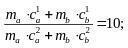
\includegraphics[width=0.8\textwidth]{assets/1099}
	\caption*{}
\end{figure} (1)

\begin{figure}[H]
	\centering
	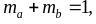
\includegraphics[width=0.8\textwidth]{assets/1100}
	\caption*{}
\end{figure} (2)

Мұндағы,

\emph{m\textsubscript{a}}, \emph{m\textsubscript{b}} -- өсімдік майының
массасы, кг;

\begin{figure}[H]
	\centering
	
\includegraphics[width=0.8\textwidth]{assets/1101}
	\caption*{}
\end{figure}, \begin{figure}[H]
	\centering
	
\includegraphics[width=0.8\textwidth]{assets/1102}
	\caption*{}
\end{figure}
-- өсімдік майындағы линол қышқылының концентрациясы, мас. \%;

\begin{figure}[H]
	\centering
	
\includegraphics[width=0.8\textwidth]{assets/1103}
	\caption*{}
\end{figure}, \begin{figure}[H]
	\centering
	
\includegraphics[width=0.8\textwidth]{assets/1104}
	\caption*{}
\end{figure}
-- өсімдік майындағы линолен қышқылының концентрациясы,~мас. \%
{[}11,12{]}.

Жүргізілген есептеулер негізінде 3-кестеде ұсынылған май қоспалары
ұсынылды.

{\bfseries 3-кесте - Қоспалардағы өсімдік майларының мөлшері}

\begin{longtable}[]{@{}
  >{\raggedright\arraybackslash}p{(\columnwidth - 6\tabcolsep) * \real{0.1777}}
  >{\raggedright\arraybackslash}p{(\columnwidth - 6\tabcolsep) * \real{0.3064}}
  >{\raggedright\arraybackslash}p{(\columnwidth - 6\tabcolsep) * \real{0.2862}}
  >{\raggedright\arraybackslash}p{(\columnwidth - 6\tabcolsep) * \real{0.2296}}@{}}
\toprule\noalign{}
\begin{minipage}[b]{\linewidth}\raggedright
Объект номері
\end{minipage} & \begin{minipage}[b]{\linewidth}\raggedright
Полиқанықпаған май қышқылдары нақты қатынасы
\end{minipage} & \begin{minipage}[b]{\linewidth}\raggedright
Мақта майы
\end{minipage} & \begin{minipage}[b]{\linewidth}\raggedright
Арыш майы
\end{minipage} \\
\midrule\noalign{}
\endhead
\bottomrule\noalign{}
\endlastfoot
Қоспа 3 & 10:1 & 0,88 & 0,12 \\
Қоспа 4 & 5:1 & 0,8 & 0,2 \\
Қоспа 5 & 3:1 & 0,65 & 0,35 \\
\end{longtable}

Қоспалар зертханалық жағдайларда алдымен екі негізгі майды араластыру
(20°C температурада магниттік араластырғышты пайдаланып тұрақты
араластыру), содан кейін қоспалардың шағын компоненттерін енгізу арқылы
алынды.

Алынған өсімдік майларының қоспаларының үлгілері олардың
органолептикалық және физико-химиялық көрсеткіштерін анықтау үшін
зерттеулерден өтті (4-кесте).

{\bfseries 4-кесте - Аралас майлардың физика-химиялық көрсеткіштері}

\begin{longtable}[]{@{}
  >{\raggedright\arraybackslash}p{(\columnwidth - 10\tabcolsep) * \real{0.1313}}
  >{\raggedright\arraybackslash}p{(\columnwidth - 10\tabcolsep) * \real{0.1524}}
  >{\raggedright\arraybackslash}p{(\columnwidth - 10\tabcolsep) * \real{0.1608}}
  >{\raggedright\arraybackslash}p{(\columnwidth - 10\tabcolsep) * \real{0.1754}}
  >{\raggedright\arraybackslash}p{(\columnwidth - 10\tabcolsep) * \real{0.1900}}
  >{\raggedright\arraybackslash}p{(\columnwidth - 10\tabcolsep) * \real{0.1900}}@{}}
\toprule\noalign{}
\begin{minipage}[b]{\linewidth}\raggedright
Қоспа саны
\end{minipage} & \begin{minipage}[b]{\linewidth}\raggedright
Қышқылдық саны,

мг КОН/г
\end{minipage} & \begin{minipage}[b]{\linewidth}\raggedright
Пероксид мәні, ½ O моль/кг
\end{minipage} & \begin{minipage}[b]{\linewidth}\raggedright
Ылғалдылық пен ұшқыш заттардың массалық үлесі, \%
\end{minipage} & \begin{minipage}[b]{\linewidth}\raggedright
Линол қышқылы құрамы, мас. \%
\end{minipage} & \begin{minipage}[b]{\linewidth}\raggedright
Линолен қышқылы құрамы, мас. \%
\end{minipage} \\
\midrule\noalign{}
\endhead
\bottomrule\noalign{}
\endlastfoot
Қоспа 1 & 0,4 & 4,4 & 0,05 & 44,73 & 5,83 \\
Қоспа 2 & 0,5 & 4,7 & 0,06 & 42,68 & 7,27 \\
Қоспа 3 & 0,4 & 3,4 & 0,06 & 41,91 & 7,60 \\
НТҚА талаптары & 4,0 & 10,0 & 0,2 & & \\
\end{longtable}

Барлық үлгілер үшін қышқыл және асқын тотығы сандары бойынша алынған
нәтижелер тазартылмаған тағамдық майлар қоспаларына қойылатын талаптарды
қанағаттандырды. Алайда, арыш майы бар үлгілерде қышқылдың да, асқын
тотығының да төмен мәндері бар екенін атап өткен жөн, бұл өндіруде,
құюда және сақтауда осы қоспалар үшін белгілі бір артықшылықтар береді.
Соған қарамастан, зерттеулердің нәтижелері өсімдік майларының барлық
ұсынылған қоспаларын өндіру мүмкіндігін дәлелдейді, өйткені олар
органолептикалық және физика-химиялық көрсеткіштері бойынша белгіленген
талаптарға толық сәйкес келеді.

Сонымен қатар, алынған өсімдік майларының қоспаларының құрамындағы ПҚМҚ
есептелген қатынасына сәйкестігі газ хроматографиясының көмегімен
бағаланды. 4 кестедегі мәліметтерден көрініп тұрғандай, линол және
линолен қышқылдарының арақатынасы күтілетін нәтижелерге толығымен сәйкес
келеді. Айта кету керек, соя майын қолданатын қоспалар әзірлеген
жағдайда, линолен қышқылына бай майларды енгізген жөн, бұл ПҚМҚ қажетті
арақатынасын қамтамасыз етуге мүмкіндік береді.

{\bfseries Қорытынды.} Сонымен қорытындылай келе, Қазақстан Республикасы
мен Ресей Федерациясының аумағында өсетін майлы дақылдардан алынатын
өсімдік майларының құрамы зерттелді. Триглицеридтердің май қышқылдарының
құрамын талдау өсімдік майларының ω-3 және ω-6 қышқылдарының қажетті
қатынасын қамтамасыз ете алмайтынын көрсетті, бұл өсімдік майларының
қоспаларын жасауды қажет етеді.

Қоспаларды алу үшін шикізат ретінде мақта және арыш майы сияқты майлар
ұсынылады. Сызықтық бағдарламалау әдісіне сүйене отырып, жұмыс
функционалды немесе профилактикалық өнім ретінде пайдалануға болатын екі
қоспаның композициясын ұсынады. Әзірленген қоспалардың композицияларына
әртүрлі пропорциядағы мақта мен арыш майы кіреді. Өсімдік майларының
қоспалары органолептикалық және физика-химиялық көрсеткіштері бойынша
белгіленген талаптарға толық сәйкес келеді. Өсімдік майларының ұсынылған
қоспаларының май қышқылдарының құрамын зерттеу адамға теңдестірілген
диетаны қамтамасыз ету үшін қажетті ω-3 және ω-6 ПҚМҚ қатынасына қол
жеткізілгенін көрсетті, бұл профилактикалық немесе емдік тамақтану үшін
қоспаларды күнделікті тұтынуға ұсынуға мүмкіндік береді.

{\bfseries Әдебиеттер}

1. Пищевая химия / А.П. Нечаев, С.Е. Траубенберг, А.А. Кочеткова {[}и
др.{]}; под ред. А.П. Нечаева. -6-е изд., стер. - СПб.: ГИОРД, 2015.-
672 с. ISBN 978-5-98879-196-6

2. Коваленко Т.Д. Инновации в предприятиях пищевой промышленности:
разработка новых видов продуктов питания // Труды международного
симпозиума «Надежность и качество». -2011. - № 1. - С.184-185.

3. ОʼБрайен Р. Жиры и масла. Производство, состав и свойства, применение
/ Р.ОʼБрайен: пер. С анг.2-го изд. В.Д.Широкова, Д.А. Бабейкиной,
Н.С.Селидановой, Н.В.Магды - СПб.: Профессия, 2007. -752 с. ISBN
978-5-93913-123-0

4. Myhrstad M. C. W., Retterstol K., Telle-Hansen V. H. Effect of marine
n-3 fatty acids on circulating inflammatory markers in healthy subjects
and subjects with cardiovascular risk factors// Inflamm Res. -2011.
-Vol. 60(4). -P. 309-319. DOI 10.1007/s00011-010-0302-5.

5. Fetterman J. W., Zdanowicz M. M. Therapeutic potential of n-3
polyunsaturated fatty acids in disease// Am J Health Syst Pharm. -2009.
-Vol. 66(13). -P. 1169-1179. DOI 10.2146/ajhp080411

6. Об утверждении Санитарных норм и правил «Требования к питанию
населения: нормы физиологических потребностей в энергии и пищевых
веществах для различных групп населения Республики Беларусь»:
постановление М-ва здравоохранения РБ, 20.11.2012, № 180 // Нац. реестр
правовых актов Респ. Беларусь. -2012. -№ 8/25580.

7. Нормы физиологических потребностей в энергии и пищевых веществах для
различных групп населения Российской Федерации. Методические
рекомендации. - М.: Федеральный центр гигиены и эпидемиологии
Роспотребнадзора. -2009. 38 с.

8. Табакаева О.В., Каланеик Т.К., Обогащенные растительные масла с
оптимизированным жирнокислотным составом // Масложировая промышленность.
-2007.-№2.-С.34-35

9. Жировые продукты для здорового питания. Современный взгляд / Л.Г.
Ипатова {[}и др.{]}. -М.: ДеЛи принт,2009. - 396 с.

10. Степычева Н.В., Фудько А.А. Купажированные растительные масла с
оптимизированным жирно-кислотным составом // Химия растительного сырья.
-2011.-№ 2.- С. 27-33.

11. Владыкина Д.С., Ламоткин С.А., Колногоров К.П., Ильина Г.Н.,
Башарова А.О. Разработка купажей растительных масел со сбалансированным
жирнокислотным составом // Труды БГТУ. -2015. - № 4. -С. 240-246. ISSN
1683-0377.

12. Lauretani, F., Bandinelli, S., Bartali, B., Cherubini, A., Iorio, A.
D., Blè, A., Giacomini, V., Corsi, A. M., Guralnik, J.M., \& Ferrucci,
L. Omega-6 and omega-3 fatty acids predict accelerated decline of
peripheral nerve function in older persons. European journal of
neurology. -2007. --Vol. 14(7). -P:. 801-808. DOI
10.1111/j.1468-1331.2007.01860.x

References

1. Pishchevaya khimiya / A.P. Nechaev, S.E. Traubenberg, A.A. Kochetkova
{[}i dr.{]}; pod red. A.P. Nechaeva. -- 6-e izd., ster. - SPb.: GIORD,
2015.- 672 s. ISBN 978-5-98879-196-6 {[}in Russian{]}

2. Kovalenko, T.D. Innovatsii v predpriyatiyakh pishchevoi
promyshlennosti: razrabotka novykh vidov produktov pitaniya // Trudy
mezhdunarodnogo simpoziuma «Nadezhnost\textquotesingle{} i kachestvo».
-2011. -- № 1. -- S.184-185. {[}in Russian{]}

3. OʼBraien R. Zhiry i masla. Proizvodstvo, sostav i svoistva,
primenenie / R.OʼBraien: per. S ang.2-go izd. V.D.Shirokova, D.A.
Babeikinoi, N.S.Selidanovoi, N.V.Magdy - SPb.: Professiya, 2007. -752 s.
ISBN 978-5-93913-123-0 {[}in Russian{]}

4. Myhrstad M. C. W., Retterstol K., Telle-Hansen V. H. Effect of marine
n-3 fatty acids on circulating inflammatory markers in healthy subjects
and subjects with cardiovascular risk factors// Inflamm Res. -2011.
-Vol. 60(4). P. 309-319. DOI 10.1007/s00011-010-0302-5.

5. Fetterman J. W., Zdanowicz M. M. Therapeutic potential of n-3
polyunsaturated fatty acids in disease// Am J Health Syst Pharm. -2009.
-Vol. 66(13). -P. 1169-1179. DOI 10.2146/ajhp080411

6. Ob utverzhdenii Sanitarnykh norm i pravil «Trebovaniya k pitaniyu
naseleniya: normy fiziologicheskikh potrebnostei v energii i pishchevykh
veshchestvakh dlya razlichnykh grupp naseleniya Respubliki
Belarus\textquotesingle»: postanovlenie M-va zdravookhraneniya RB,
20.11.2012, № 180 // Nats. reestr pravovykh aktov Resp.
Belarus\textquotesingle. -2012. -№ 8/25580. {[}in Russian{]}

7. Normy fiziologicheskikh potrebnostei v energii i pishchevykh
veshchestvakh dlya razlichnykh grupp naseleniya Rossiiskoi Federatsii.
Metodicheskie rekomendatsii. - M.: Federal\textquotesingle nyi tsentr
gigieny i epidemiologii Rospotrebnadzora. -2009. 38 s. {[}in Russian{]}

8. Tabakaeva O.V., Kalaneik T.K., Obogashchennye
rastitel\textquotesingle nye masla s optimizirovannym zhirnokislotnym
sostavom // Maslozhirovaya promyshlennost\textquotesingle.
-2007.-№2.-S.34-35 {[}in Russian{]}

9. Zhirovye produkty dlya zdorovogo pitaniya. Sovremennyi vzglyad / L.
G. Ipatova {[}i dr.{]}. -M.: DeLi print,2009. - 396 s. {[}in Russian{]}

10. Stepycheva N.V., Fud\textquotesingle ko A.A. Kupazhirovannye
rastitel\textquotesingle nye masla s optimizirovannym zhirno-kislotnym
sostavom // Khimiya rastitel\textquotesingle nogo
syr\textquotesingle ya. -2011. -№2. -S. 27-33. {[}in Russian{]}

11. Vladykina D.S., Lamotkin S.A., Kolnogorov K.P.,
Il\textquotesingle ina G.N., Basharova A.O. Razrabotka kupazhei
rastitel\textquotesingle nykh masel so sbalansirovannym zhirnokislotnym
sostavom // Trudy BGTU. -2015. - № 4. -S. 240-246. ISSN 1683-0377. {[}in
Russian{]}

12. Lauretani, F., Bandinelli, S., Bartali, B., Cherubini, A., Iorio, A.
D., Blè, A., Giacomini, V., Corsi, A. M., Guralnik, J.M., \& Ferrucci,
L. Omega-6 and omega-3 fatty acids predict accelerated decline of
peripheral nerve function in older persons. European journal of
neurology. -2007. --Vol. 14(7). -P:. 801-808. DOI
10.1111/j.1468-1331.2007.01860.x

\emph{{\bfseries Авторлар туралы мәліметтер}}

Отуншиева А.Е. - Әл-Фараби атындағы Қазақ Ұлттық университетінің
«Жылуфизика және техникалық физика» кафедрасы «Стандарттау және
сертификаттау» білім беру бағдарламасының докторанты, Алматы, Қазақстан,
e-mail: 03.08.1990.43@mail.ru;

Ламоткин С.А. - Беларусь мемлекеттік технологиялық университет,
«Физика-химиялық әдістер және сапаны қамтамасыз ету» кафедрасының
меңгерушісі, х.ғ.к., доценті,~ Минск, Беларуссия, e‑mail:
jossby@rambler.ru ;

Болегенова С.А. - Әл-Фараби атындағы Қазақ Ұлттық Университеті,
«Жылуфизика және техникалық физика» кафедрасының меңгерушісі,
ф.-м.ғ.д.,профессоры, Алматы, Қазақстан, e‑mail:
saltanat.bolegenova@kaznu.kz;

Ветохин С.С. {\bfseries -} Беларусь мемлекеттік технологиялық университеті,
«Физика-химиялық әдістер және сапаны қамтамасыз ету» кафедрасы,
ф.-м.ғ.к., профессоры, Минск, Беларуссия, e‑mail: serega49@mail.ru;

Ешанкулов А.А. {\bfseries -} М.Ауезов атындағы Оңтүстік Қазақстан Зерттеу
Университеті, «Механика және мұнайгаз ісі» факульетінің декан
орынбасары, «Стандарттау және сертификаттау» кафедрасының т.ғ.к.,
доценті, Шымкент, Қазақстан, e‑mail: amirkhan-74@mail.ru.

\emph{{\bfseries Сведения об авторах}}

Otunshiyeva A.E.. - doctoral student of the educational programme
«Standardisation and Certification», department of «Thermal physics and
technical physics», Kazakh National University named after Al-Farabi,
Almaty, Kazakhstan, e-mail: 03.08.1990.43@mail.ru;

Lamotkin S.A. - Head of the Department «Physico-chemical methods and
quality assurance» of the Belarusian State Technological University,
Candidate of Chemical Sciences, Associate Professor, Minsk, Belarus,
e-mail: jossby@rambler.ru;

Bolegenova S.A. - Head of the Department of `Thermophysics and Technical
Physics', Kazakh National University named after Al-Farabi, Dr. Ph.
Almaty, Kazakhstan, e-mail: saltanat.bolegenova@kaznu.kz;

Vetokhin S.S. - Belarusian State Technological University, Department of
«Physico-chemical methods and quality assurance», Candidate of Physical
and Chemical Sciences, Professor, Minsk, Belarus, e-mail:
serega49@mail.ru;

Esankulov A.A. - deputy dean of the faculty «Mechanics and oil and gas
business» of M. Auezov South Kazakhstan Research University, Candidate
of Science, associate professor of the department `Standardisation and
Certification', Shymkent, Kazakhstan, e-mail: amirkhan-74@mail.ru.\newpage
{\bfseries МРНТИ 65.09.03}

{\bfseries STUDYING EFFECT OF FREEZE DRYING ON THE CHEMICAL COMPOSITION OF
COW COLOSTRUM}

{\bfseries T.Ch. Tultabayeva, G.N Zhakupova, N.Kokumbekova, A.T.Sagandyk,}

{\bfseries A.H. Muldasheva, A.T.Akhmetzhanova}

NJSC "Kazakh Agrotechnical Research University named after S.
Seifullin",

Astana, Kazakhstan

Corresponding author: aygerim\_talgatqyzy@mail.ru

The article presents studies of the quality of cow colostrum. To date, a
promising direction in the development of food functional products
technology is the processing of cow colostrum as an additional source of
protein, immunoglobulins, lipids, vitamins, minerals and other
biologically active substances. It has been established that the
physico-chemical composition of colostrum depends on the time elapsed
since the calving of the cow. According to the conducted studies, it was
found that the protein content is significantly higher in colostrum
obtained immediately after calving than in colostrum collected after 24
hours and 36 hours after calving. The article provides data on the study
of dry cow colostrum obtained by freeze-drying. In this regard, the
authors of the article investigated the chemical composition of dry
colostrum, namely, the concentration of protein, fat and ash was
determined depending on the time of collection of colostrum. The authors
found that colostrum obtained immediately after calving also has low
humidity, which makes it possible to increase the shelf life. The
article substantiates the ways of its subsequent use in the production
of food products with high nutritional and biological value and possible
immunomodulatory effect.

{\bfseries Key words:} cow colostrum, dry colostrum, biologically active
substances, proteins.

{\bfseries ИССЛЕДОВАНИЕ ВЛИЯНИЯ СУБЛИМАЦИОННОЙ СУШКИ НА ХИМИЧЕСКИЙ СОСТАВ
КОРОВЬЕГО МОЛОЗИВА}

{\bfseries T.Ч. Тултабаева, Г. Н. Жакупова, Н. Кокумбекова, А. Т.
Сагандык,}

{\bfseries А. Х. Мулдашева, А. Т. Ахметжанова}

НАО «Казахский агротехнический исследовательский университет им. Сакена
Сейфуллина» , Астана, Казахстан,

e-mail: aygerim\_talgatqyzy@mail.ru

В представленной статье рассмотрены исследования качества коровьего
молозива. На сегодняшний день перспективным направлением развития
технологии пищевых функциональных продуктов является переработка
молозива коров как дополнительного источника белка, иммуноглобулинов,
липидов, витаминов, минеральных и других биологически активных веществ.
Установлено, что физико-химический состав молозива зависит от времени,
прошедшего с момента отела коровы. В соответствии с проведенными
исследованиями обнаружено, что содержание белка существенно выше в
молозиве, полученном сразу после отела, чем в молозиве собранном после
24 часов и 36 часов с момента отела. В статье приводятся данные по
исследованию сухого коровьего молозива, полученного методом
сублимационной сушки. В связи с этим авторами статьи исследован
химический состав сухого молозива, а именно определена концентрация
белка, жира и золы в зависимости от времени сбора молозива. Авторами
установлено, что молозиво, полученное сразу после отела имеет также
низкую влажность, что дает возможность увеличения сроков хранения. В
статье обоснованы пути последующего его использования в производстве
пищевой продукции с высокой пищевой и биологической ценностью и
возможным иммуномодулирующим действием.

{\bfseries Ключевые слова:} коровье молозиво, сухое молозиво, биологически
активные вещества, белки.

{\bfseries СУБЛИМАЦИЯЛЫҚ КЕПТІРУДІҢ СИЫР УЫЗЫНЫҢ ХИМИЯЛЫҚ ҚҰРАМЫНА ӘСЕРІН
ЗЕРТТЕУ}

{\bfseries Тултабаева Т.Ч., Жакупова Г.Н., Кокумбекова Н., Сағандық А.Т.,}

{\bfseries Мулдашева А.Х., Ахметжанова А.Т.}

\textsuperscript{1} КеАҚ «С.Сейфуллин атындағы Қазақ агротехникалық
зерттеу университеті»,

Астана, Қазақстан,

*e-mail: aygerim\_talgatqyzy@mail.ru

Ұсынылған мақалада сиыр уызының сапасы туралы зерттеулер қарастырылған.
Бүгінгі таңда тағамдық функционалды өнімдер технологиясын дамытудың
перспективалы бағыты сиырдың уыз сүтін ақуыздың, иммуноглобулиндердің,
липидтердің, дәрумендердің, минералды және басқа да биологиялық белсенді
заттардың қосымша көзі ретінде өңдеу болып табылады. Уыздың
физика-химиялық құрамы сиырды төлдегеннен кейінгі уақытқа байланысты
екендігі анықталды. Жүргізілген зерттеулерге сәйкес, ақуыздың мөлшері
төлдегеннен кейін бірден алынған уыз сүтінде төлдегеннен кейін 24 сағат
36 сағаттан кейін жиналған уыз сүтіне қарағанда айтарлықтай жоғары
екендігі анықталды. Мақалада мұздатып кептіру әдісімен алынған құрғақ
сиыр уызын зерттеу туралы мәліметтер келтірілген. Осыған байланысты
мақала авторлары құрғақ уыздың химиялық құрамын зерттеді, атап айтқанда
уыз сүтін жинау уақытына байланысты ақуыз, май және күл концентрациясы
анықталды. Авторлар төлдегеннен кейін бірден алынған уыздың ылғалдылығы
төмен екенін анықтады, бұл сақтау мерзімін ұзартуға мүмкіндік береді.
Мақалада оны кейіннен тағамдық және биологиялық құндылығы жоғары және
иммуномодуляциялық әсері бар тамақ өнімдерін өндіруде қолдану жолдары
негізделген.

{\bfseries Түйін сөздер:} сиыр уызы, құрғақ уыз, биологиялық белсенді
заттар, ақуыздар.

{\bfseries Introduction.} The nutraceuticals and functional foods market
shows significant progress aimed to meet consumer demand. Nowadays,
people are looking for new and safer food ingredients that become not
only a source of nutrients, but also benefit health and ensure
well-being. This concept draws consumers\textquotesingle{} attention to
dietary biologically active compounds, nutraceuticals and functional
foods.

One of the underestimated biologically active product with great
potential is cow colostrum. Nowadays it is of great interest of
scientists from all over the world {[}1{]}. Cow colostrum is a feed or
abnormal milk, that rich in immunological agents, play the role of
passive immunity in a newborn calf, guarantee of protection and help in
the development of the gastrointestinal system {[}2{]}. Its composition
rich in dry substances, proteins, immunoglobulins, fats and growth
factors, which arouses interest in their use in the development of both
pharmaceuticals and food derivatives {[}3{]}.

A.G. Khramtsov et al. studied protective substances (antibacterial
factors) of cow colostrum. The authors believe that colostrum is useful
not only for newborn calves, but also for children, athletes, the
elderly, patients with tuberculosis, stomach ulcers and diabetes
{[}4{]}. It is known that colostrum contains in its composition a
significant amount of lactoferrin, lactoperoxidase and lysozyme, which
have antimicrobial and antiviral properties. Lactoperoxidase affects the
binding of liposaccharides by regulating bacterial growth, while
lactoferrin has toxic properties for several gram-positive and negative
bacteria, as well as antiviral properties. Meanwhile lysozyme affect to
the health by attacking the peptidoglycan component of gram-positive
bacteria, causing bacterial lysis {[}5{]}. By gaining such positive
effects colostrum allow to destruct certain pathogenic microorganisms
such as E. coli, rotavirus and cryptosporidium {[}6{]}.

The use of colostrum remains limited not only due to insufficient
research of this biologically active substance, but also due to its
short shelf life. The technology of deep processing and obtaining acid
preservation, dry concentrate on its basis, or isolation and
purification of individual fractions without significant changes in
composition and quality are expensive and time-consuming {[}7{]}. Due to
the development of mini-refrigerators, the preservation and
transportation market of colostrum, the processing point is not
technically difficult anymore and ensures the preservation of all
biologically valuable substances {[}8{]}.

Thus, the above discussion approved that the direction of scientific
research as the development of food products based on milk colostrum
becomes relevant.

The aim of the work was to study the physico-chemical parameters of
colostrum of Simmental cows and compare the composition of natural
colostrum and colostrum powder obtained by freeze drying.

{\bfseries Materials and methods.} This part should consist of a
description of the materials, the progress of the work, as well as a
complete description of the used methods. The characterization or
description of the research material includes the presentation of the
specified material in qualitative and quantitative terms. The
characteristic of the material is one of the factors determining the
reliability of the conclusions and research methods.

Objects and methods of research

- colostrum of Simmental cows obtained after calving, after 24 hours and
36 hours

- dry colostrum obtained by freeze-drying in the laboratory.

The research of the physico-chemical composition was carried out in the
research laboratory of the Food Technology and Processing Products
department of the S. Seifullin Kazakh Agrotechnical Research University.

The following methods were used in the process of conducting the study:

- titrated acidity -- according to State Standart 3624-92 "Milk and
dairy products. Methods for determining titrated acidity"; {[}9{]}.

-protein content in natural and dry colostrum -- according to State
Standart 25179-2014 "Milk and dairy products. Methods for determining
the mass fraction of protein";{[}10{]}.

- fat content -- according to State Standart 5867-90 "Milk and dairy
products. Methods for determining fat";{[}11{]}.

- moisture content on moisture meters RADWAG MA -60.3;

- lactose and solids content -- on the TANGO BRUKER spectrophotometer
with a measuring range of 11500-4000 cm\textsuperscript{-1}.

{\bfseries Results and discussion.} In order to determine the
physico-chemical composition of cow colostrum, raw material were taken
from the most common Simmental cow breed in the Akmola region. For the
purity of the experiment, cows kept under equal conditions and received
the same amount of feed while milking.

It has been established that cow colostrum is a breast milk of the
mammary gland, produced after calving for enhanced feeding of the calf
in the first days of life and providing it with a large number of
antibodies for the formation of natural immunity. It is produced in the
postpartum period during the next 7-10 days after calving. Young animals
that received the first portion of colostrum within 1.5 hours after
birth, up to 2 weeks, show relatively better growth rates and are immune
to general dyspepsia and bronchopneumonia {[}12{]}.

The first batch of colostrum was received within 3 hours after calving,
then the second batch after 24 hours and the third batch after 36 hours.
Visually, natural colostrum is a yellow-brown liquid on the first day of
milking, which by the third day approaches the color of milk. The
physico-chemical composition of natural cow colostrum is presented in
Table 1.

{\bfseries Table 1- Physico-chemical composition of natural cow colostrum}

\begin{longtable}[]{@{}
  >{\raggedright\arraybackslash}p{(\columnwidth - 8\tabcolsep) * \real{0.0534}}
  >{\raggedright\arraybackslash}p{(\columnwidth - 8\tabcolsep) * \real{0.3102}}
  >{\raggedright\arraybackslash}p{(\columnwidth - 8\tabcolsep) * \real{0.1970}}
  >{\raggedright\arraybackslash}p{(\columnwidth - 8\tabcolsep) * \real{0.1970}}
  >{\raggedright\arraybackslash}p{(\columnwidth - 8\tabcolsep) * \real{0.2424}}@{}}
\toprule\noalign{}
\begin{minipage}[b]{\linewidth}\raggedright
№№
\end{minipage} & \begin{minipage}[b]{\linewidth}\raggedright
Parameters
\end{minipage} & \begin{minipage}[b]{\linewidth}\raggedright
Colostrum

after calving
\end{minipage} & \begin{minipage}[b]{\linewidth}\raggedright
Colostrum

after 24 hours
\end{minipage} & \begin{minipage}[b]{\linewidth}\raggedright
Colostrum

after 36 hours
\end{minipage} \\
\midrule\noalign{}
\endhead
\bottomrule\noalign{}
\endlastfoot
1 & Titrable acidity, \textsuperscript{0} Т & 58 & 40 & 32 \\
2 & рН & 4,92 & 6,41 & 6,49 \\
3 & Dry matters, \% & 19,17 & 10,80 & 10,04 \\
4 & Protein content, \% & 13,34 & 7,54 & 3,95 \\
5 & Lactoze, \% & 5,54 & 4,76 & 4,51 \\
6 & Fat content, \% & 5,08 & 4,48 & 2,95 \\
7 & Moisture, \% & 63,976 & 78,588 & 79,731 \\
8 & Purity (group) &
\multicolumn{3}{>{\raggedright\arraybackslash}p{(\columnwidth - 8\tabcolsep) * \real{0.6364} + 4\tabcolsep}@{}}{%
No less than II} \\
9 & Temperature, \textsuperscript{0} С &
\multicolumn{3}{>{\raggedright\arraybackslash}p{(\columnwidth - 8\tabcolsep) * \real{0.6364} + 4\tabcolsep}@{}}{%
4*/-2} \\
\end{longtable}

According to the data given in Table 1, it was found that the results
comply with State Standart R -- 71167-2023 ``Cow colostrum (raw
materials). Technical conditions''{[}13{]}. The data shows that the
chemical composition of colostrum depends on the time of the cow's
calving. According to the data, after calving, the percentage of
protein, fat and lactose is 13.34:5.08:5.54\% compared with colostrum
obtained on the second day of milking, which is 10.8:4.48:4.76\%.
According to the analysis data and based on the organoleptic properties,
it was found that colostrum obtained after 36 hours after calving is
close to the indicators of cow\textquotesingle s milk and thus its study
has no scientific interest.

Considering that colostrum can be stored at a temperature from 0
\textsuperscript{0}C to 4 \textsuperscript{0}C for up to 8 days, subject
to sanitary requirements, without significantly changing the nutritional
value of colostrum. Colostrum was freeze-dried to preserve the
biological and nutritional properties. Drying was carried out in
laboratory conditions in Vacuum freeze-drier LG -06 at a temperature of
- 50 \textsuperscript{0}C and a pressure of 10 MPa.

In the resulting dry colostrum physico-chemical composition were
assesed. The data are shown in Table 2.

{\bfseries Table 2 - Physico-chemical composition of dry cow colostrum}

\begin{longtable}[]{@{}
  >{\raggedright\arraybackslash}p{(\columnwidth - 8\tabcolsep) * \real{0.0534}}
  >{\raggedright\arraybackslash}p{(\columnwidth - 8\tabcolsep) * \real{0.3102}}
  >{\raggedright\arraybackslash}p{(\columnwidth - 8\tabcolsep) * \real{0.1970}}
  >{\raggedright\arraybackslash}p{(\columnwidth - 8\tabcolsep) * \real{0.1970}}
  >{\raggedright\arraybackslash}p{(\columnwidth - 8\tabcolsep) * \real{0.2424}}@{}}
\toprule\noalign{}
\begin{minipage}[b]{\linewidth}\raggedright
№№
\end{minipage} & \begin{minipage}[b]{\linewidth}\raggedright
Parameters
\end{minipage} & \begin{minipage}[b]{\linewidth}\raggedright
Colostrum

after calving
\end{minipage} & \begin{minipage}[b]{\linewidth}\raggedright
Colostrum

after 24 hours
\end{minipage} & \begin{minipage}[b]{\linewidth}\raggedright
Colostrum

after 36 hours
\end{minipage} \\
\midrule\noalign{}
\endhead
\bottomrule\noalign{}
\endlastfoot
1 & Titrable acidity, \textsuperscript{0} Т & 57 & 42 & 35 \\
2 & Protein content, \% & 37,3 & 32,2 & 29,2 \\
3 & Lactoze, \% & 5,5 & 4,7 & 4,1 \\
4 & Ashes, \% & 6,9 & 5,4 & 5,2 \\
5 & Fat content, \% & 39,7 & 32,2 & 28,3 \\
6 & Moisture, \% & 3,51 & 3,92 & 3,91 \\
\end{longtable}

The resulting dry colostrum has real prospects for use as a functional
ingredient in food products.

{\bfseries Conclusions.} The results of studies of the chemical composition
of colostrum prove the prospects of its use in the food industry as a
source of protein of animal origin. However, it should be borne in mind
that the maximum amount of biologically active substances is stored in
colostrum in the first hours after calving.

This work was carried out within the framework of the IRN BR21882184
2PCF-MNVO/24 program "Creation of a set of risk management measures to
ensure food safety and the development of meat and dairy products with
increased biological value"

{\bfseries References}

\begin{enumerate}
\def\labelenumi{\arabic{enumi}.}
\item
  Bodammer, P., Maletzki, C., Waitz, G., \& Emmrich, J. Prophylactic
  application of bovine colostrum ameliorates murine colitis via
  induction of immunoregulatory cell // Journal of Nutrition. -2011.
  --Vol. 141(6). --P. 1056-1061. DOI 10.3945/jn.110.128702
\item
  Nikolic, I., Stojanovic, I., Vujicic, M., Fagone, P., Mangano, K.,
  Stosic-Grujicic, S., Nicoletti, F., \& Saksida, T. Standardized bovine
  colostrum derivative impedes development of type 1 diabetes in rodents
  // Immunobiology. -2017. --Vol. 222(2). --P. 272-279. DOI
  10.1016/j.imbio.2016.09.013
\item
  McSweeney, P. L. H., \& McNamara, J. P. Encyclopedia of Dairy
  Sciences: Third edition. In Encyclopedia of Dairy Sciences: Third
  edition. -2021.
\item
  Gorbatova K.K. Biokhimiya moloka i molochnykh produktov. - SPb.:
  GIORD, 2001. - 320 s. {[}in Russian{]}
\item
  Bagwe, S., Tharappel, L. J. P., Kaur, G., \& Buttar, H. S. Bovine
  colostrum: An emerging nutraceutical // In Journal of Complementary
  and Integrative Medicine. -2015. -Vol. 12. --Iss. 3. DOI
  10.1515/jcim-2014-0039
\item
  Mehra, R., Singh, R., Nayan, V., Buttar, H. S., Kumar, N., Kumar, S.,
  Bhardwaj, A., Kaushik, R., \& Kumar, H. Nutritional attributes of
  bovine colostrum components in human health and disease: A
  comprehensive review // In Food Bioscience. -Vol. 40. DOI
  10.1016/j.fbio.2021.100907
\item
  Pat. 2275564 Rossiiskaya Federatsiya. MPK F 26 V 9/06 Transfer Faktor
  XF™ Patent SShA №4 816 563. Sposob polucheniya sublimirovannykh
  pishchevykh produktov. -№ 77.99.23.3.U.7085.12.04 ot 10.12.04. {[}in
  Russian{]}
\item
  Pat.2535877 S1 Rossiiskaya Federatsiya. MPK A23/S 9/123. Cposob
  proizvodstva iogurta s funktsional\textquotesingle nymi svoistvami /
  Polyanskaya Irina Sergeevna, Topal Ol\textquotesingle ga Ivanovna,
  Novokshanova Alla L\textquotesingle vovna, Teraevich Alla Sergeevna. -
  № 2013134767/10, 2013.07.23; zayavl. 23.07.2013; opubl. 20.12.2014
  {[}in Russian{]}
\item
  Leont\textquotesingle eva S.A., Tikhonov S.L., Tikhonova N.V., Lazarev
  V.A. Korov\textquotesingle e molozivo - perspektivnoe
  syr\textquotesingle e dlya proizvodstva produktov pitaniya //
  Pishchevaya promyshlennost\textquotesingle. -2021. --T. 6. -№2. - S.
  23-33. {[}in Russian{]}
\end{enumerate}

10.GOST 3624-92. Moloko i molochnye produkty. Titrim etricheskie m etody
opredeleniya kislotnosti. --M: Standartinform, 2009. -6s. {[}in
Russian{]}

11. GOST 25179-2014 Moloko i molochnye produkty. Metody opredeleniya
massovoi doli belka. --M: Standartinform, 2015. -8s. {[}in Russian{]}

12. GOST 5867-90 Moloko i molochnye produkty. Metody opredeleniya zhira.
--M: Standartinform, 2009. -12s. {[}in Russian{]}

13. GOST R-71167-2023. Molozivo korov\textquotesingle\textquotesingle e
(syr\textquotesingle\textquotesingle e) Tekhnicheskie usloviya. --M:
Ross. Inst.standartizatsii. -14 s. {[}in Russian{]}

\emph{{\bfseries Information about the authors}}

Tultabayeva T.Ch. -- d.t.n., associate professor, Kazakh Agrotechnical
Research University named after S.Seifullin, Astana, Kazakhstan, e-mail:
tamara\_tch@list.ru;

Zhakupova G.N. -- candidate of technical sciences,Kazakh Agrotechnical
Research University named after S.Seifullin, Astana, Kazakhstan, e-mail:
gulmira-zhak@mail.ru;

Kokumbekova N.K.- master of technical sciences, Kazakh Agrotechnical
Research University named after S.Seifullin, Astana, Kazakhstan, e-mail:
kokumbekovanazym@gmail.ru;

Sagandyk A.T. -- master of technical sciences, S.Seifullin Kazakh
Agrotechnical Research University, Astana, Kazakhstan, e-mail:
assema.bukeyeva@gmail.com;

Muldasheva A.H. -- master of technical sciences Kazakh Agrotechnical
Research University named after S.Seifullin, Astana, Kazakhstan, e-mail:
Ak91.91@mail.ru;

Akhmetzhanova A.T. -- doctoral student ,Kazakh Agrotechnical Research
University named after S.Seifullin, Astana, Kazakhstan, e-mail:
aygerim\_talgatqyzy@mail.ru

\emph{{\bfseries Сведения об авторах}}

Тултабаева T.Ч.- д.т.н, ассоц. профессор, Казахский агротехнический
исследовательский университет им.С.Сейфуллина, Астана, Казахстан,
e-mail: tamara\_tch@list.ru;

Жакупова Г.Н. -- к.т.н., ассоц. профессор, Казахский агротехнический
исследовательский университет им.С.Сейфуллина, Астана, Казахстан,
e-mail: gulmira-zhak@mail.ru;

Кокумбекова Н.К.- магистр технических наук, Казахский агротехнический
исследовательский университет им.С.Сейфуллина, Астана, Казахстан,
e-mail: kokumbekovanazym@gmail.ru;

Сагандык А.Т. -- магистр технических нау Казахский агротехнический
исследовательский университет им.С.Сейфуллина, младший» Астана,
Казахстан, e-mail: assema.bukeyeva@gmail.com;

Мулдашева А.Х. -- магистр технических наук, Казахский агротехнический
исследовательский университет им.С.Сейфуллина, Астана, Казахстан,
e-mail: Ak91.91@mail.ru;

Ахметжанова А.Т. -- докторант кафедры Казахский агротехнический
исследовательский университет им.С.Сейфуллина», Астана, Казахстан,
e-mail: aygerim\_talgatqyzy@mail.ru\newpage
{\bfseries IRSTI 65.33.91}

{\bfseries INCREASING OF MICROBIOLOGICAL STABILITY OF BREAD WITH USING
SECONDARY RAW MATERIALS FROM CEREAL PROCESSING}

{\bfseries \textsuperscript{1}M.Zh. Yessembek, B.K.
Tarabayev\textsuperscript{1}, \textsuperscript{2}A.M. Omaraliyeva}

\textsuperscript{1}NCJSC S.Seifullin Kazakh Agro Technical Research
University, Astana, Kazakhstan,

\textsuperscript{2}JSC Kazakh University of Technology and Business
named after K. Kulazhanov, Astana, Kazakhstan,

Corresponding author: aygerim\_talgatqyzy@mail.ru

Bread and bakery products are one of the main food products, and their
quality does not always meet the requirements of modern nutrition
science. One of the directions of solving this problem is the creation
of new safe varieties of bakery products of functional purpose to
correct the nutrition of the population. The article considers the
causes of microbial spoilage, the negative influence of mold fungi and
spore-forming bacteria of the genus \emph{Bacillus} on the safety of
bread with the use of secondary raw materials of grain crops processing.
The main objects of research were bakery products with the use of rice
and buckwheat brans, prepared by the traditional method and on complex
sourdough starter. Studies on the influence of the method of rice and
buckwheat brans application on resistance to mold and potato disease
infection were conducted.

{\bfseries Keywords:} Microbiological safety, bread, secondary raw
materials, rice bran, buckwheat bran, fermented brew, mold, potato
disease.

{\bfseries ДӘНДІ ДАҚЫЛДАРДЫ ҚАЙТА ӨҢДЕУДІҢ ЕКІНШІЛІК ШИКІЗАТЫН ҚОЛДАНА
ОТЫРЫП НАННЫҢ МИКРОБИОЛОГИЯЛЫҚ ТҰРАҚТЫЛЫҒЫН АРТТЫРУ}

{\bfseries \textsuperscript{1}М.Ж. Есембек, \textsuperscript{1}Б.К.
Тарабаев, \textsuperscript{2}А.М. Омаралиева}

\textsuperscript{1} С.Сейфуллин атындағы Қазақ агротехникалық зерттеу
университеті» КеАҚ,

Астана, Қазақстан,

\textsuperscript{2}Қ. Құлажанов атындағы Қазақ технология және бизнес
университеті АҚ,

Астана, Қазақстан

e-mail: yessembek.madina@gmail.com

Нан және нан өнімдері негізгі тағамдардың бірі болып табылады және
олардың сапасы қазіргі заманғы тамақтану ғылымының талаптарына әрдайым
сәйкес келе бермейді. Бұл мәселені шешудің бір бағыты -- халықтың
тамақтануын түзету үшін функционалды мақсаттағы нан өнімдерінің жаңа
қауіпсіз сорттарын әзірлеу. Мақалада дәнді дақылдарды қайта өңдеудің
екіншілік шикізатын қолдана отырып нанның қауіпсіздігіне микробтардың
бүліну себептері, зең саңырауқұлақтары мен \emph{Bacillus} тектес спора
түзетін бактериялардың кері әсері қарастырылады. Негізгі зерттеу
нысандары дәстүрлі әдіспен және кешенді ашытқымен дайындалған күріш және
қарақұмық ұншығынан жасалған нан өнімдері болды. Күріш және қарақұмық
ұншығын енгізу әдісінің көгеруге және картоп ауруына төзімділігіне әсері
бойынша зерттеулер жүргізілді.

{\bfseries Түйін сөздер:} Микробиологиялық қауіпсіздік, нан, екіншілік
шикізат, күріш ұншығы, қарақұмық ұншығы, ашытылған қайнатпа, көгеру,
картоп ауруы.

{\bfseries ПОВЫШЕНИЕ МИКРОБИОЛОГИЧЕСКОЙ УСТОЙЧИВОСТИ ХЛЕБА С ПРИМЕНЕНИЕМ
ВТОРИЧНОГО СЫРЬЯ ПЕРЕРАБОТКИ ЗЕРНОВЫХ КУЛЬТУР}

{\bfseries \textsuperscript{1}М.Ж. Есембек, \textsuperscript{1}Б.К.
Тарабаев, \textsuperscript{2}А.М. Омаралиева}

\textsuperscript{1}НАО «Казахский агротехнический исследовательский
университет им. С.Сейфуллина, Астана, Казахстан,

\textsuperscript{2}АО Казахский университет технологии и бизнеса им.К.
Кулажанова,

Астана, Казахстан

e-mail: yessembek.madina@gmail.com

Хлеб и хлебобулочные изделия являются одним из основных продуктов
питания, а их качество далеко не всегда соответствует предъявляемым
требованиям современной науки о питании. Одним из направлений решения
данной проблемы является создание новых безопасных сортов хлебобулочных
изделий функционального назначения для коррекции питания населения. В
статье рассмотрены причины микробной порчи, отрицательное влияние
плесневых грибов и спорообразующих бактерий рода \emph{Bacillus} на
безопасность хлеба с применением вторичного сырья переработки зерновых
культур. Основными объектами исследований выступали хлебобулочные
изделия с использованием рисовой и гречневой мучек, приготовленные
традиционным способом и на комплексной закваске. Проведены исследования
по влиянию способа внесения рисовой и гречневой мучек на устойчивость к
плесневению и заражению картофельной болезнью.

{\bfseries Ключевые слова:} Микробиологическая безопасность, хлеб,
вторичное сырье, рисовая мучка, гречневая мучка, заквашенная заварка,
плесневение, картофельная болезнь.

{\bfseries Introduction.} In the modern world food production is put on a
stream, a stable process of production of high-quality bakery products
is impossible without the purposeful use of food additives, improvers,
various types of raw materials. They have a wide functional range, have
the properties to affect the components of raw materials, give a certain
quality to finished products, increase nutritional value, and also give
the opportunity to form certain properties of dough from flour with
unstable baking characteristics.

Ingredients, with the help of which it is possible to increase the
nutritional value of wheat bread, are currently very diverse. The most
appropriate is the use of non-traditional ingredients of plant origin,
containing a high amount of proteins, micro and macronutrients. When
they are used, the therapeutic and preventive value of wheat bread
increases {[}1, 2{]}. One of such ingredients is rice and buckwheat bran
{[}3{]}. These raw materials contain a wide range of biologically active
substances, which, when added to food, have a beneficial effect on the
human body.

Analysis of scientific and industrial developments indicate that there
are numerous studies on the use of secondary raw materials of cereal
crops for enrichment of bakery products. However, currently a serious
problem of bakery products is their vulnerability to microbial spoilage
under the action of bacteria and mold fungi, as it not only leads to
deterioration of the appearance of bakery products, but also negatively
affects their quality and safety.

The most dangerous and widespread disease of bread is considered to be
potato disease, which is often observed in regions with hot climate and
in summer time. In recent years, due to the widespread use of packaging
in polymeric materials, which is a provoking factor for the development
of microbial spoilage, the spread of cases of potato disease is noted
not only in the southern regions, but also in the northern regions of
Kazakhstan and in the spring-summer period, and in winter {[}4, 5{]}.
The causative agents of this disease are spore-forming bacteria of the
genus \emph{Bacillus}. Spores of potato bread disease pathogens, unlike
mold fungi, are able to persist in the finished product after baking.

Affected bread first loses its natural taste and aroma, then a peculiar
sweetish odor appears in it, which as the disease develops intensifies
and the smell of bread acquires a rotten tinge. Under the influence of
active enzymes of the causative agent of potato bread disease, there are
significant changes in the structure of the bread crumb: dark smearing
and pulling threads appear inside.

The second common type of microbial spoilage of bakery products is mold,
which occurs as a result of the development of mold fungi of the genera
\emph{Aspergillus (А. fiavus, А. fumigatus, А. glaucus, А. nidulans, А.
niger, А. ochaceus), Mucor (М. mucedo, М. pusillus, М. spinosus),
Penicillium (Р. crustosum, Р. expansum), Rhizopusnigricans,
Geotrichumcandidum.} The surface of bread affected by mold is covered
with fluffy plaque of various colors: gray, white, green, yellow,
bluish, black {[}6{]}. The bread comes out of the oven sterile, i.e.
mold is a secondary contamination.

Mould fungi adversely affect the quality of raw materials and finished
bread. They cause profound changes in bread by breaking down proteins,
carbohydrates and fats with the help of their enzymes. Bread that is
affected by mold fungi has an unpleasant taste and musty odor. About 80
species of mold fungi produce mycotoxins. Mycotoxins can cause health
problems in people who consume bread affected by mold fungi {[}7{]}.

A promising step in combating microbial spoilage of bread using
secondary raw materials of cereal crop processing is the use of
substances of natural origin that have a preserving effect, such as
metabolites of lactic acid bacteria, such as organic acids and
bacteriocins. The use of sourdough starters to inhibit microbial
spoilage of bread has been the subject of much research in recent years.
It is proved that bread prepared on sourdough starter with directed
cultivation is characterized by improved porosity structure and crumb
properties, taste and odor, microbiological purity, ability to preserve
freshness for a long time. The use of sourdough starter bred on pure
cultures of starter microorganisms allows to increase microbiological
safety and quality of bread.

In this regard, the research on the development of bread assortment with
the use of secondary raw materials of grain crops processing of improved
quality, increased nutritional value and microbiological stability is
relevant.

The purpose of the present research was to study the influence of the
method of rice and buckwheat brans application on the resistance of
bakery products to mold and potato disease development.

{\bfseries Materials and methods.} The research was carried out on the
basis of the ``Laboratory of innovative technologies and assortment of
bakery products'' of the St. Petersburg branch of the Federal State
Autonomous Scientific Institution ``Research Institute of Baking
Industry''. The objects of research were bakery products with the use of
rice and buckwheat brans, prepared by traditional method and on complex
sourdough starter. The control sample of bread was prepared without the
addition of rice and buckwheat brans by the method of trial laboratory
baking.

In the traditional method, 5\% rice bran and 10\% buckwheat bran in dry
form and 85\% first grade wheat flour, salt and pressed baking yeast,
sugar according to the recipe and water in the amount providing dough
moisture 48.0\% were added to the dough.

When preparing dough on complex sourdough starter, the sourdough starter
was prepared in accordance with the ``Collection of technological
instructions for the production of bakery products'' {[}8,9{]}, bred on
pure cultures of microorganisms in liquid form.

The peculiarity of the preparation of dough on complex sourdough starter
is the use of complex sourdough starter, by fermenting of sugared brew
at a temperature of 32-34°C. Also using a composition of pure cultures
of starter microorganisms. These compositions have probiotic properties
and antibiotic action against spore microflora. At the same time,
traditional biological starters (thick, liquid without brewing, liquid
with brewing) are excluded from the technological process, the amount of
flour introduced in brewed form (25-35\%) is increased.

Preparation of complex sourdough starter includes dilution and
production cycles.

For preparation of complex sourdough starter were used pure cultures of
lactic acid bacteria \emph{L.plantarum 1, L. brevis E120,} (1.5 ml each)
and yeast \emph{S.cerevisiae st. L-1} (1 ml of aqueous suspension).

The dilution cycle was used with a small mass of sourdough starter (500
g in the first phase). Microbial cultures were fused together, added to
the saccharified brew of rice and buckwheat brans with the addition of
unfermented barley malt (2\% to the weight of brans) and water, and left
to ferment for 20 hours.

The complex sourdough starter bred by breeding cycle using pure cultures
of lactic acid bacteria and starter yeast in liquid form in the
production cycle was maintained by refreshing with sugared brew in the
ratio of 1:1 - 1:9, i.e. complex sourdough starter - nutrition (sugared
brew) depending on the duration of sourdough starter fermentation.

80\% of the complex sourdough starter obtained was used for bread
production and the remaining part (20\%) was used for its refreshing.

To establish the influence of bread preparation technology on the rate
of mold development, we conducted model experiments with the infection
of its sterile slices with pure culture of mold fungi \emph{Penicillium
chrysogenum} {[}10,11{]}.

To determine the possibility of suppressing the potato disease of bread,
the method of putting finished products infected with spore bacteria
into conditions provoking the development of \emph{B. subtilis} was
used. To create provoking conditions, dry bread crumbs infected with
\emph{B. subtilis} spore-forming bacteria and containing
10\textsuperscript{8} KOE/g of spores were introduced during dough
kneading. To determine the content of \emph{B. subtilis} spores in the
infected crumb, the method described in the book ``Microbiology of
Baking Production'' (Afanasyeva O.V., 2003) was used {[}12{]}. Bread was
stored according to the Instruction for the prevention of potato bread
disease {[}13{]}, for which immediately after baking the bread was
wrapped in damp paper and placed in a thermostat at 37°C. After 24
hours, the bread was cut with a knife and the presence of signs of
disease (specific unpleasant odor, sticky crumb) was determined
visually. In the absence of the disease, the bread was further incubated
under the same conditions.

{\bfseries Results and discussion.} In the preparation of bread using rice
and buckwheat brans by the traditional method, it was found that the use
of secondary raw materials in dry form provokes the growth of mold fungi
during the storage of bread compared to products prepared on complex
sourdough starter and without the addition of secondary raw materials.

At infection of sterile bread slices with rice and buckwheat brans on
complex sourdough starter, pure culture of mold \emph{Penicillium
chrysogenum}, mold spores did not appear, which proves that the use of
secondary raw materials in the form of fermented brew during dough
kneading provides its microbiological purity, especially resistance of
bread to mold. At the same time on the surface of bread slices prepared
with rice and buckwheat brans in dry form, mold growth was observed
after 26 hours. While on a slice of control bread, prepared from
first-grade wheat flour without the addition of secondary raw materials,
mold spores appeared after 28 hours (Fig. 1).

{\bfseries Figure 1- Effect of rice and buckwheat brans application method
on bread resistance to moldiness}

Considering that the biological method involving the use of acidifying
components is one of the most effective ways to protect bread from
potato blight, the effect of rice and buckwheat brans on the suppression
of potato bacillus spores was investigated.

As a result of trial baking it was found that the appearance of signs of
potato disease after 10 hours in the form of unpleasant odor and after
14 hours - stickiness of the crumb, was observed in the sample of bread
prepared with the addition of rice and buckwheat brans in dry form. In
the control sample of bread prepared from first grade wheat flour
without the addition of secondary raw materials, unpleasant odor and
stickiness of the crumb appeared after 19 and 25 hours, respectively.
The bread sample with the addition of rice and buckwheat brans in the
form of fermented brew did not get potato disease (Fig. 2).

{\bfseries Figure 2 - Effect of rice and buckwheat brans application method
on resistance to potato bread disease}

As a result of the conducted research it was found that the introduction
of rice and buckwheat brans in the form of fermented brew increases
antagonistic activity to \emph{Bacillus subtilis} and completely
suppresses the development of spores of potato bacillus.

{\bfseries Conclusions.} According to the results of studies of
microbiological indicators of bread quality it was found that the
application of secondary products of cereal crops: rice and buckwheat
brans in the form of fermented brew increases the resistance of bread to
mold and completely suppresses the development of potato disease. This
indicates that the introduction of secondary products of cereal crops in
the form of fermented brew has a significant effect on microbial
spoilage of bread, compared to traditional methods of bread preparation.
The results of the research can be recommended for use in the
development of multicomponent products based on secondary raw materials,
namely rice and buckwheat bran. This will improve the range of products
and diversify the nutrition of consumers seeking a healthy lifestyle.

{\bfseries References}

1. Nikiforova T.A., Khon I.A., Baikov V.G. Ratsional\textquotesingle noe
ispol\textquotesingle zovanie vtorichnogo syr\textquotesingle ya
krupyanogo proizvodstva. // Khleboprodukty. -- 2014. - №6. -- S. 50-51.
{[}in Russian{]}

2. Nikiforova T.A., Khon I.A. Vliyanie grechnevoi muchki na sokhranenie
svezhesti khleba. // Khleboprodukty. - 2017. - №6. -- S.38-39. {[}in
Russian{]}

3. Esembek M.Zh., Tarabaev B.K., Omaralieva A.M., Botbaeva Zh.T.,
Kakimov M.M. Nan өndіrіsіnde paidalanu үshіn dәndі -- daқyldardy қaita
өңdeudің ekіnshіlіk shikіzatyn zertteu // Almaty tekhnologiyalyқ
universitetіnің khabarshysy. - 2022. - №1. - C. 29-35. DOI
10.48184/2304-568X-2022-1-29-35 {[}in Kazakh{]}

4. Dudikova D. Problemy kartofel\textquotesingle noi bolezni khleba v
Kazakhstane//Khleboprodukty. -- 2001. - № 11. -C. 23-26. {[}in
Russian{]}

5. Polyakova S.P. Metody i sredstva povysheniya mikrobiologicheskoi
bezopasnosti khlebobulochnykh izdelii // Khlebopechenie Rossii. - 2003.
- № 6. - S. 3-5. {[}in Russian{]}

6. Frolova Yu.M., Savkina O.A, Lokachuk M.N., Pavlovskaya E.N.,
Kuznetsova L.I., Parakhina O.I. Zakvaska kak sredstvo obespecheniya
mikrobiologicheskoi bezopasnosti khlebobulochnykh izdelii // Povyshenie
kachestva i bezopasnosti pishchevykh produktov: Materialy XII
Vserossiiskoi nauchno-prakticheskoi konferentsii s mezhdunarodnym
uchastiem, posvyashchennoi 90-letiyu so dnya rozhdeniya doktora
tekhnicheskikh nauk, professora, Zasluzhennogo deyatelya nauki RF M.S.
Aminova, Makhachkala, 09--10 noyabrya 2022 goda. -- Makhachkala. --
2022. -- S. 110-112. {[}in Russian{]}

7. Dzh. M. Dzhei. Sovremennaya pishchevaya mikrobiologiya / Dzh. M.
Dzhei, M. Dzh. Messner, D. A. Gol\textquotesingle den.- M.: BINOM.
Laboratoriya znanii, 2017. --- 886 s. ISBN 978-5-9963-1300-6 {[}in
Russian{]}

8. Sbornik sovremennykh tekhnologii khlebobulochnykh izdelii / pod
obshchei redaktsiei chlen-korrespondenta Rossiiskoi akademii
sel\textquotesingle skokhozyaistvennykh nauk A. P. Kosovana. -- M. : GNU
GOSNII khlebopekarnoi promyshlennosti, 2008. -- 268 s. {[}in Russian{]}

9. Pat. 7716 RK MPK A21D 8/02. Sposob prigotovleniya zakvaski dlya
proizvodstva khleba / M.Zh. Esembek, B.K. Tarabaev, L.I.Kuznetsova, A.M.
Omaralieva, Zh.T. Botbaeva. -№ 2022/0944.2; zayavl. 30.10.2022; opubl.
06.01.2023; Byul. №1. {[}in Russian{]}

10. Kuznetsova L.I, Savkina O.A., Ivanova E.S., Usova L.V., Ternovskoi
G.V. O plesnevenii khleba // Khlebopechenie Rossii. - 2014. - № 5. - S.
24-26. {[}in Russian{]}

11. Dubrovskaya N.O., Kuznetsova L.I., Savkina O.A. Vliyanie novoi
podkislyayushchei smesi na kachestvo rzhano-pshenichnogo khleba,
vyrabatyvaemogo po uskorennoi tekhnologii. // Khlebopechenie Rossii -
2014. - № 2. - S. 21-22. {[}in Russian{]}

12. Afanas\textquotesingle eva, O. V. Mikrobiologiya khlebopekarnogo
proizvodstva / O.V. Afanas\textquotesingle eva; S.-Peterb. fil. Gos.
nauch.-issled. in-ta khlebopekar. prom-sti (SPb F GosNIIKhP). - SPb. :
Beresta, 2003. - 220 s. {[}in Russian{]}

13. Instruktsiya po preduprezhdeniyu kartofel\textquotesingle noi
bolezni khleba na khlebopekarnykh predpriyatiyakh. -- M.: GNU GOSNIIKhP
Rossel\textquotesingle khozakademii, 2012. -- 32 s. {[}in Russian{]}

\emph{{\bfseries Information about authors}}

Yessembek M.ZH. - Master of Technical sciences, NCJSC S.Seifullin Kazakh
Agro Technical Research University, Astana, Kazakhstan, e-mail:
yessembek.madina@gmail.com;

Tarabayev B.K. - Candidate of Technical Sciences, NCJSC S.Seifullin
Kazakh Agro Technical Research University, Astana, Kazakhstan, e-mail:
b.tarabayev@kazatu.edu.kz;

Omaraliyeva A.M. {\bfseries -} Candidate of Technical Sciences, JSC Kazakh
University of Technology and Business named after K. Kulazhanov, Astana,
Kazakhstan, e-mail: aigul-omar@mail.ru

\emph{{\bfseries Авторлар туралы мәліметтер}}

Есембек М.Ж -- техника ғылымдарының магистрі, С.Сейфуллин атындағы Қазақ
агротехникалық зерттеу университеті КеАҚ, Астана, Қазақстан, e-mail:
yessembek.madina@gmail.com;

Б.К. Тарабаев - техника ғылымдарының кандидаты, «С.Сейфуллин атындағы
Қазақ агротехникалық зерттеу университеті КеАҚ, Астана қ., Қазақстан,
e-mail: b.tarabayev@kazatu.edu.kz;

Омаралиева А.М. - техника ғылымдарының кандидаты, Қ. Құлажанов атындағы
Қазақ технология және бизнес университеті АҚ, Астана, Қазақстан, e-mail:
aigul-omar@mail.ru